\section*{第六章 多面体和旋转体}

1. B 提示: $\left\{  \begin{array}{l} \text{ 直平行六面体: 底面是平行四边形, } \\  \text{ 长方体: 底面是正方形, } \\  \text{ 正四棱柱: 底面是正方形, } \\  \text{ 正四棱柱: 底面是正方形, } \\  \text{ 直四棱柱: 底面是四边形, } \end{array}\right.$ 它们的侧棱都垂直于底面. $\because$ (正方形) $\subset  \{$ 平行四边形 $\}  \subset  \{$ 四

边形 $\} ,\;\therefore \;C \subset  B \subset  A \subset  D\therefore$ 选 $B$ .

2. D 提示:长方体:底面是矩形且侧棱垂直于底面, $\therefore$ 选 D.

3. D 提示: 如图, $\because \angle {FEH} = {60}^{ \circ  },\therefore {EF} = {FH} = {HE}$ ,即 ${FH} = H{H}_{1} = {H}_{1}{F}_{1} = {F}_{1}F$ . 连接 ${EG},\because \angle {E}_{1}{EF} = \angle {E}_{1}{EH},\therefore$ 点 ${E}_{1}$ 在底面的射影落在直线 ${EG}$ 上. 过 ${E}_{1}$ 作 ${EA} \bot$  ${EG}$ 于点 $A.\because {EG} \bot  {HF},\therefore$ 由三垂线定理, ${E}_{1}E \bot  {HF}$ . 又 $\because {E}_{1}E//{F}_{1}F$ ,

\begin{center}
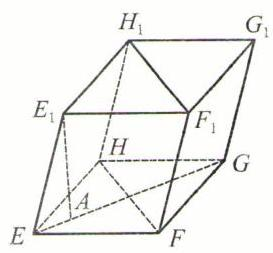
\includegraphics[width=0.2\textwidth]{bodyxb/src/bo_d20cdrf7aajc73bfmvhg_142_1246_495_273_253_0.jpg}
\end{center}


(第 3 题)

$\therefore {F}_{1}F \bot  {HF},\therefore$ 四边形 ${H}_{1}{HF}{F}_{1}$ 为正方形. $\therefore$ 选 D.

4. $B$ 提示: $S = 2\left( {{ac} + {bc}}\right)  = {2c} \cdot  \left( {a + b}\right) ,\;\therefore$ 选 $B$ .

5. B 提示: 设同一顶点出发的三条棱长为 $x,y,z$ . 则对角线 $= \sqrt{{x}^{2} + {y}^{2} + {z}^{2}} =$  $\sqrt{\dfrac{\left( {{x}^{2} + {y}^{2}}\right)  + \left( {{y}^{2} + {z}^{2}}\right)  + \left( {{x}^{2} + {z}^{2}}\right) }{2}} = \sqrt{\dfrac{{a}^{2} + {b}^{2} + {c}^{2}}{2}},\;\therefore \;$ 选 B.

6. $C$ 提示:如图甲,在正三棱柱 ${ABC} - {A}_{1}{B}_{1}{C}_{1}$ 中, $H,{H}_{1}$ 分别为 ${BC},{B}_{1}{C}_{1}$ 的中点. 考虑矩形 ${AH}{H}_{1}{A}_{1}$ (如图乙),在 ${AH},{A}_{1}{H}_{1}$ 上分别取 $P,{P}_{1}$ ,使 ${PH} =$  $\dfrac{1}{3}{AH},{P}_{1}{H}_{1} = \dfrac{1}{3}{A}_{1}{H}_{1}$ ,取 $P{P}_{1}$ 的中点 $O$ ,连接 ${HO}$ 并延长,交 ${A}_{1}{H}_{1}$ 于点 $M$ . 在图甲中作出点 $M$ ,过点 $M$ 作 ${B}_{1}{C}_{1}$ 的平行线,分别交 ${A}_{1}{B}_{1},{A}_{1}{C}_{1}$ 于点 $E,F$ ,平面 ${EFCB}$ 即为截面. 故选 C.

\begin{center}
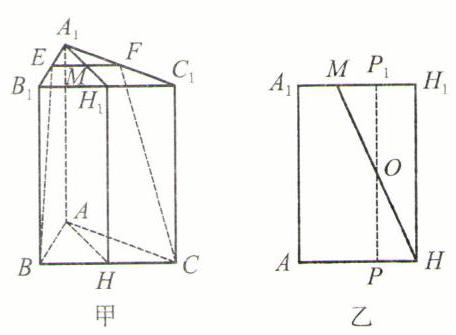
\includegraphics[width=0.3\textwidth]{bodyxb/src/bo_d20cdrf7aajc73bfmvhg_142_1069_816_456_335_0.jpg}
\end{center}


(第 6 题)

7. $B$ 提示:对角线 $= \sqrt{{a}^{2} + {a}^{2} + \left( {{b}^{2} - {a}^{2}}\right) } = \sqrt{{a}^{2} + {b}^{2}},\;\therefore$ 选 B.

8. $B$ 提示: 如图,由已知, ${NP} \bot  P{P}_{1}$ . 又 ${NP} \bot  {PM}$ ,

$\therefore {NP} \bot$ 面 ${M}_{1}{P}_{1}{PM}$ .

$\because {MP} \subset$ 面 ${M}_{1}{P}_{1}{PM},\therefore {NP} \bot  {M}_{1}P$ ,

$\therefore \;\sin \beta  = \dfrac{PN}{{M}_{1}N}$ . 又 $\cos \theta  = \dfrac{MN}{{M}_{1}N},\sin \alpha  = \dfrac{PN}{MN}$ ,

$\therefore \cos \theta  \cdot  \sin \alpha  = \dfrac{PN}{{M}_{1}N}$ ,即 $\sin \beta  = \cos \theta  \cdot  \sin \alpha .\;\therefore$ 选 B.

\begin{center}
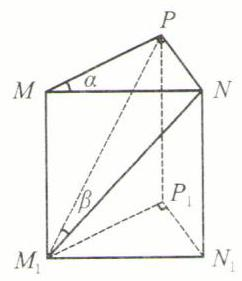
\includegraphics[width=0.2\textwidth]{bodyxb/src/bo_d20cdrf7aajc73bfmvhg_142_562_1348_242_281_0.jpg}
\end{center}


(第 8 题)

\begin{center}
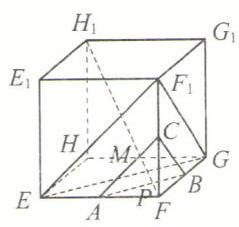
\includegraphics[width=0.2\textwidth]{bodyxb/src/bo_d20cdrf7aajc73bfmvhg_142_888_1398_239_227_0.jpg}
\end{center}


(第 9 题)

9. B 提示: 如图 $\bigtriangleup {ABC}$ 为所求截面,则 $\bigtriangleup {ABC} \backsim  \bigtriangleup {EG}{F}_{1}$ ,且分别交 $F{H}_{1}$ 于点 $P,M.{V}_{F - {EC}{F}_{1}} = {V}_{E - {FC}{F}_{1}} \Rightarrow  \dfrac{1}{3} \cdot  {S}_{\bigtriangleup E{F}_{1}} \cdot  {FM}$  $= \dfrac{1}{3} \cdot  {S}_{\bigtriangleup {FG}{F}_{1}} \cdot  {FE} \Rightarrow  {FM} = \dfrac{\sqrt{3}}{3}$ . 又 ${FP} = \dfrac{P{H}_{1}}{5} = \dfrac{F{H}_{1}}{6} = \dfrac{\sqrt{3}}{6}$ ,

$\therefore \dfrac{{S}_{\bigtriangleup {ABC}}}{{S}_{\bigtriangleup {EG}{F}_{1}}} = {\left( \dfrac{FP}{FM}\right) }^{2} = {\left( \dfrac{\dfrac{\sqrt{3}}{6}}{\dfrac{\sqrt{3}}{3}}\right) }^{2} = {\left( \dfrac{1}{2}\right) }^{2} = \dfrac{1}{4} \Rightarrow  {S}_{\bigtriangleup {ABC}} = \dfrac{\sqrt{3}}{4}{\left( \sqrt{2}\right) }^{2} \cdot  \dfrac{1}{4} = \dfrac{\sqrt{3}}{8},\;\therefore$ 选 B.

10. (1) 22 提示: $\left\{  \begin{array}{l} {a}^{2} + {b}^{2} + {c}^{2} = {14}, \\  4\left( {a + b + c}\right)  = {24}, \end{array}\right.$

由②得 $a + b + c = 6$ ,

即 ${\left( a + b + c\right) }^{2} = {36} \Rightarrow  {a}^{2} + {b}^{2} + {c}^{2} + {2ab} + {2bc} + {2ac} = {36}$ ,

③一①得. ${S}_{\Delta } = 2\left( {{ab} + {bc} + {ac}}\right)  = {22}$ .

(2) $\sqrt{14}$ 提示: $\left\{  {\begin{array}{l} 2\left( {{ab} + {bc} + {ac}}\right)  = {22}, \\  4\left( {a + b + c}\right)  = {24} \end{array} \Rightarrow  {a}^{2} + {b}^{2} + {c}^{2} = {14}}\right.$ . $\therefore$ 对角线长 $\sqrt{14}$ .

(3)8,6,24提示:由题设长、宽、高分别为 ${4k},{3k},{12k}$ . 则 ${\left( 4k\right) }^{2} + {\left( 3k\right) }^{2} + {\left( {12}k\right) }^{2} = {26}^{2} \Rightarrow  k = 2$ ,

$\therefore$ 长、宽、高分别为8,6,24.

(4) $\sqrt{6}$ 提示: ${ab} = \sqrt{2},{ac} = \sqrt{3},{bc} = \sqrt{6} \Rightarrow  a = 1,b = \sqrt{2},c = \sqrt{3},\therefore$ 对角线长为 $\sqrt{{a}^{2} + {b}^{2} + {c}^{2}} = \sqrt{6}$ .

11. (1) $\dfrac{\sqrt{7}}{4}{a}^{2}$ 提示:如图, $S = \dfrac{1}{2} \cdot  a \cdot  \dfrac{\sqrt{7}}{2}a = \dfrac{\sqrt{7}}{4}{a}^{2}$ .

(2) $8\sqrt{3}$ 提示:如图, $S = \dfrac{1}{2} \cdot  4 \cdot  4\sqrt{3} = 8\sqrt{3}$ .

(3) ${90}^{ \circ  }$ 提示:如图,延长 ${BA}$ 至点 $M$ ,使 ${AM} = {B}_{1}{A}_{1}$ ,连接 ${CM}$ , ${A}_{1}M$ ,由余弦定理可得 ${MC} = \sqrt{5}a$ . 在 $\bigtriangleup  M{A}_{1}C$ 中, ${A}_{1}M$  $= \sqrt{3}a,{MC} = \sqrt{5}a,{A}_{1}C = \sqrt{2}a$ . 则 ${A}_{1}{C}^{2} + {A}_{1}{M}^{2} = M{C}^{2},\therefore \angle M{A}_{1}C = {90}^{ \circ  }$ ,即 ${A}_{1}M\bot {A}_{1}C$ . 又 ${A}_{1}M//{B}_{1}A$ , $\therefore A{B}_{1}\bot {A}_{1}C$ ,即所成角为 ${90}^{ \circ  }$ .

\begin{center}
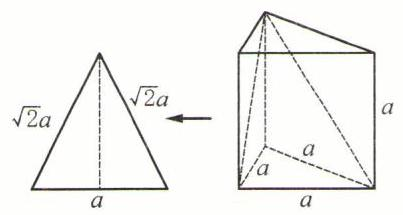
\includegraphics[width=0.3\textwidth]{bodyxb/src/bo_d20cdrf7aajc73bfmvhg_143_231_629_403_215_0.jpg}
\end{center}


[第 11(1)题]

\begin{center}
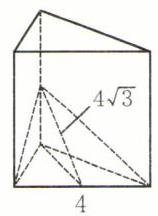
\includegraphics[width=0.2\textwidth]{bodyxb/src/bo_d20cdrf7aajc73bfmvhg_143_709_623_158_216_0.jpg}
\end{center}


[第 11(2)题]

\begin{center}
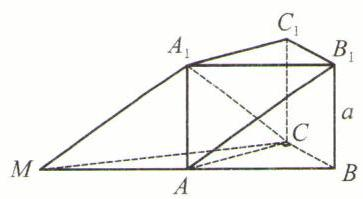
\includegraphics[width=0.3\textwidth]{bodyxb/src/bo_d20cdrf7aajc73bfmvhg_143_945_640_363_199_0.jpg}
\end{center}


[第 11(3)题]

(4) $2\sqrt{6}$ 或 $\sqrt{66}$ 提示: $\sqrt{{4}^{2} + {2}^{2} + {2}^{2}} = 2\sqrt{6},\sqrt{{8}^{2} + {1}^{2} + {1}^{2}} = \sqrt{66}$ .

(5) $\dfrac{2}{3}a$ 提示: 如图, $h = \dfrac{\dfrac{\sqrt{2}}{2}a \cdot  {2a}}{\sqrt{{\left( \dfrac{\sqrt{2}}{2}a\right) }^{2} + {\left( 2a\right) }^{2}}} = \dfrac{2}{3}a$ .

(6) $\sqrt{3}{a}^{2}$ 或 $2{a}^{2}$ 提示:如图, ${S}_{1} = a \cdot  \sqrt{3}a = \sqrt{3}{a}^{2}\;{S}_{2} = a \cdot  {2a} = 2{a}^{2},\;\therefore$ 对角面的面积为 $\sqrt{3}{a}^{2}$ 或 $2{a}^{2}$ . 12. (1) 设底面菱形的两条对角线长分别为 $a,b$ . 则 $\left\{  {\begin{array}{l} {a}^{2} + {5}^{2} = {9}^{2}, \\  {b}^{2} + {5}^{2} = {15}^{2} \end{array} \Rightarrow  \left\{  \begin{array}{l} a = 2\sqrt{14}, \\  b = {10}\sqrt{2}. \end{array}\right. }\right.$ 则底面边长 $= \sqrt{{\left( \sqrt{14}\right) }^{2} + {\left( 5\sqrt{2}\right) }^{2}} = 8$ . (2)设底面菱形的对角线长分别为 ${3k},{4k}$ . 则高为 $\dfrac{1}{k}$ ,菱形边长为 $\dfrac{5}{2}k,\;\therefore \;{S}_{\text{ 侧 }} = \dfrac{5}{2}k \times  \dfrac{1}{k} \cdot  4 = {10}$ . (3)设底面菱形的对角线长分别为 $a,b$ ,高为 $h$ . $\left\{  {\begin{array}{l} {\left( \dfrac{a}{2}\right) }^{2} + {\left( \dfrac{b}{2}\right) }^{2} = {8}^{2}, \\  {50}\sqrt{2} = {ah}, \\  {10}\sqrt{14} = {bh} \end{array} \Rightarrow  \left\{  \begin{array}{l} a = {10}\sqrt{2}, \\  b = 2\sqrt{14}, \\  h = 5, \end{array}\right. }\right.$  $\therefore$ 对角线长为 $\sqrt{{a}^{2} + {h}^{2}} = {15}$ 和 $\sqrt{{b}^{2} + {h}^{2}} = 9$ . (4)如图,由题意可得 ${A}_{1}{D}_{1} = 3,{A}_{1}{B}_{1} = 5,\angle {D}_{1}{A}_{1}{B}_{1} = {60}^{ \circ  }$ , $\therefore {B}_{1}{D}_{1} = \sqrt{19}$ , $\therefore B{D}_{1} = \sqrt{{B}_{1}{D}_{1}^{2} + B{B}_{1}^{2}} = \sqrt{35}$ . 同理, $A{C}_{1} = \sqrt{65}$ .

\begin{center}
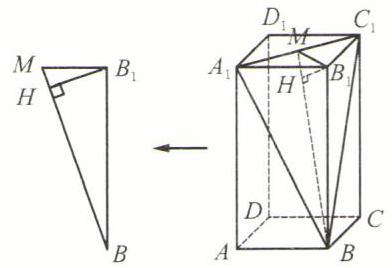
\includegraphics[width=0.3\textwidth]{bodyxb/src/bo_d20cdrf7aajc73bfmvhg_143_377_1158_392_268_0.jpg}
\end{center}


[第 11(5)题]

\begin{center}
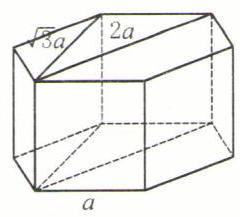
\includegraphics[width=0.2\textwidth]{bodyxb/src/bo_d20cdrf7aajc73bfmvhg_143_874_1208_240_217_0.jpg}
\end{center}


[第 11(6)题]

\begin{center}
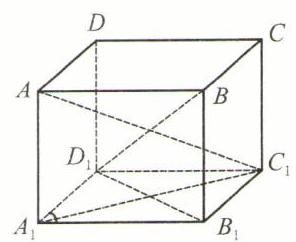
\includegraphics[width=0.2\textwidth]{bodyxb/src/bo_d20cdrf7aajc73bfmvhg_143_1132_1813_296_242_0.jpg}
\end{center}


[第 12(4)题]

(5)如图,在 $\mathrm{{Rt}}\bigtriangleup {D}_{1}{DB}$ 中, ${D}_{1}B = l,\angle {D}_{1}{BD} = {45}^{ \circ  }$ ,可得 ${D}_{1}D = \dfrac{\sqrt{2}}{2}l$ . 在 $\mathrm{{Rt}}\bigtriangleup B{C}_{1}{D}_{1}$ 中 ${D}_{1}B = l,\angle {D}_{1}B{C}_{1} = {30}^{ \circ  }$ ,

\begin{center}
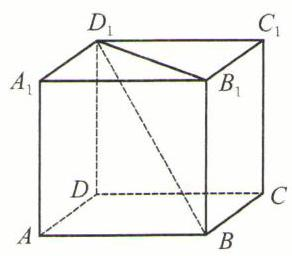
\includegraphics[width=0.2\textwidth]{bodyxb/src/bo_d20cdrf7aajc73bfmvhg_144_1217_122_292_256_0.jpg}
\end{center}


[第 12(5)题]

$\therefore \;{D}_{1}{C}_{1} = \dfrac{1}{2}l,\;\therefore \;{A}_{1}{D}_{1} = \sqrt{{l}^{2} - {\left( \dfrac{\sqrt{2}}{2}l\right) }^{2} - {\left( \dfrac{1}{2}l\right) }^{2}} = \dfrac{1}{2}l$ .

${S}_{\text{ 全 }} = 2\left( {\dfrac{\sqrt{2}}{2}l \cdot  \dfrac{1}{2}l + \dfrac{1}{2}l \cdot  \dfrac{1}{2}l + \dfrac{1}{2}l \cdot  \dfrac{\sqrt{2}}{2}l}\right)  = \left( {\dfrac{1}{2} + \sqrt{2}}\right) {l}^{2}.$

13. (1) 如图,过 ${C}_{1}$ 作 ${C}_{1}H \bot  {A}_{1}{B}_{1}$ 于 $H$ ,连接 ${BH}$ . 由题意可得 ${C}_{1}H \bot$ 平面 ${A}_{1}{AB}{B}_{1}$ ,

$\therefore \angle {C}_{1}{BH}$ 即所成角. 在 $\mathrm{{Rt}} \bigtriangleup  {C}_{1}{HB}$ 中, ${C}_{1}H = \dfrac{\sqrt{3}}{2},{BH} = \dfrac{\sqrt{5}}{2},\therefore \tan \theta  = \dfrac{\sqrt{15}}{5}$ .

\begin{center}
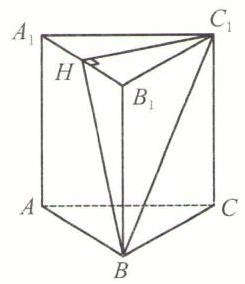
\includegraphics[width=0.2\textwidth]{bodyxb/src/bo_d20cdrf7aajc73bfmvhg_144_553_527_245_284_0.jpg}
\end{center}


[第 13(1)题]

\begin{center}
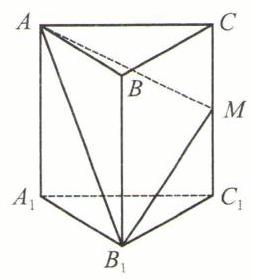
\includegraphics[width=0.2\textwidth]{bodyxb/src/bo_d20cdrf7aajc73bfmvhg_144_905_531_253_280_0.jpg}
\end{center}


[第 13(2)题]

( 2 )如图, $\bigtriangleup A{B}_{1}M$ 在底面的射影即 $\bigtriangleup {A}_{1}{B}_{1}{C}_{1},\therefore \cos \theta  = \dfrac{{S}_{\bigtriangleup {A}_{1}{B}_{1}{C}_{1}}}{{S}_{\bigtriangleup A{B}_{1}M}} = \dfrac{\dfrac{\sqrt{3}}{4}}{\dfrac{\sqrt{6}}{4}} = \dfrac{\sqrt{2}}{2},\therefore \theta  = {45}^{ \circ  }$ .

14. B 提示:选项 $\left( A\right) \left( C\right) \left( D\right)$ 的反例,底面为菱形(其中有一个角为 ${60}^{ \circ  }$ )的直平行六面体.

$\therefore$ 选 B.

15. B 提示:如图,① $\because A{A}_{1}{C}_{1}C$ 为矩形 $\therefore A{A}_{1} \bot  {AC}$ .

\begin{center}
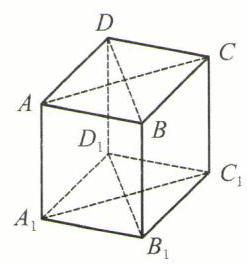
\includegraphics[width=0.2\textwidth]{bodyxb/src/bo_d20cdrf7aajc73bfmvhg_144_1265_1096_247_264_0.jpg}
\end{center}


(第 15 题)

又 $\because B{B}_{1}{D}_{1}D$ 为矩形,

$\therefore B{B}_{1} \bot  {BD}$ . 又 $A{A}_{1}//B{B}_{1}$ ,

$\therefore A{A}_{1} \bot  {BD},\therefore A{A}_{1} \bot$ 平面 ${ABCD}$ ,

$\therefore$ 是直平行六面体. 同理可得②④错误,③正确. $\therefore$ 选 B.

16. $B$ 提示:如图,设正方体 ${ABCD} - {A}_{1}{B}_{1}{C}_{1}{D}_{1}$ 的棱长为 1. 则 ${S}_{\text{ 正方体全 }} = {1}^{2} \times  6 = 6$ ,

则正四面体 $B - {A}_{1}{C}_{1}{D}_{1}$ 的棱长为 $\sqrt{2}.{S}_{\text{ 正四面体全 }} = \dfrac{\sqrt{3}}{4} \cdot  {\left( \sqrt{2}\right) }^{2} \cdot  4 = 2\sqrt{3}$ ,

$\therefore \dfrac{{S}_{\text{ 正方体全 }}}{{S}_{\text{ 正四面体全 }}} = \dfrac{6}{2\sqrt{3}} = \sqrt{3}$ ,

$\therefore$ 选 B.

\begin{center}
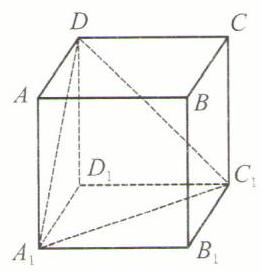
\includegraphics[width=0.2\textwidth]{bodyxb/src/bo_d20cdrf7aajc73bfmvhg_144_350_1550_262_273_0.jpg}
\end{center}


(第 16 题)

\begin{center}
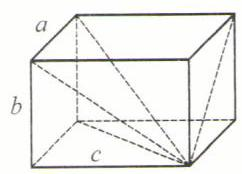
\includegraphics[width=0.2\textwidth]{bodyxb/src/bo_d20cdrf7aajc73bfmvhg_144_696_1644_242_174_0.jpg}
\end{center}


(第 17 题)

\begin{center}
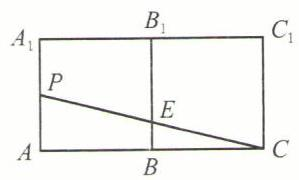
\includegraphics[width=0.2\textwidth]{bodyxb/src/bo_d20cdrf7aajc73bfmvhg_144_1022_1633_299_180_0.jpg}
\end{center}


(第 19 题)

17. B 提示: 如图, ${\cos }^{2}\alpha  + {\cos }^{2}\beta  + {\cos }^{2}\beta  = \dfrac{{a}^{2} + {c}^{2}}{{a}^{2} + {b}^{2} + {c}^{2}} + \dfrac{{a}^{2} + {b}^{2}}{{a}^{2} + {b}^{2} + {c}^{2}} + \dfrac{{b}^{2} + {c}^{2}}{{a}^{2} + {b}^{2} + {c}^{2}} = 2,\;\therefore$ 选B.

18. $B$ 提示:以 $O,P$ 为相对顶点作长方体,该长方体的边分别平行 (或重合于三个平面的交线),设所求角为 $\theta$ ,则由第 17 题的结论, ${\cos }^{2}{60}^{ \circ  } + {\cos }^{2}{60}^{ \circ  } + {\cos }^{2}\theta  = 1$ ,得 $\cos \theta  = \dfrac{\sqrt{2}}{2}$ ,故 $\theta  = {45}^{ \circ  }.\;\therefore {OP}$ 与 ${l}_{3}$ 所成角为 ${45}^{ \circ  }.\;\therefore$ 选 B.

19. $C$ 提示:如图,把平面 ${BC}{C}_{1}{B}_{1}$ 展开,可得 ${\left( PE + EC\right) }_{\min } = {PC},\therefore \left| {PC}\right|  = \dfrac{\sqrt{17}}{2}$ ,选 C.

20. D 提示: 如图, ${AD}$ 与 ${DE},{DF}$ 所成的角均为 ${60}^{ \circ  }.{S}_{\text{ 面 }{AF}} = {S}_{\text{ 面 }{AE}} = \cos {60}^{ \circ  } \cdot  {AD} \cdot  {DE} = {10}\sqrt{3}.{S}_{\text{ 面 }{BCFE}} = 4 \times  5 = {20}.{S}_{\text{ 侧 }} = 2$  $\times  {10}\sqrt{3} + {20} = {20}\left( {\sqrt{3} + 1}\right) ,\;\therefore \;$ 选 D. 21. (1) 如图,设截面 ${ADE}$ 与底面 ${ABC}$ 所成的角为 $\theta$ ,则 $\cos \theta  = \dfrac{{S}_{\bigtriangleup {ABC}}}{{S}_{\bigtriangleup {ADE}}} = \dfrac{AC}{AE} = \dfrac{\sqrt{2}}{2},\therefore \theta  = {45}^{ \circ  }$ . ( 2 )如图,延长 ${ED},{CB}$ ,交于点 $F$ ,设点 $C$ 到截面 ${ADE}$ 距离为 $h$ ,则 $h = \dfrac{{S}_{\bigtriangleup {ACF}} \cdot  {CE}}{{S}_{\bigtriangleup {AEF}}} = \dfrac{\sqrt{3}}{\sqrt{6}}a = \dfrac{\sqrt{2}}{2}a$ . 22. (1) ${S}_{\text{ 侧 }} = 2 \times  \left( {\dfrac{\sqrt{2}}{2}b \times  a}\right)  + {ab} = \left( {\sqrt{2} + 1}\right) {ab}$ . (2) ${S}_{\text{ 全 }} = 6 \times  \dfrac{\sqrt{3}}{4}{a}^{2} + {a}^{2} = \left( {\dfrac{3\sqrt{3}}{2} + 1}\right) {a}^{2}$ . (3) ${S}_{\text{ 侧 }} = a \times  \dfrac{\sqrt{3}}{2} \times  \dfrac{\sqrt{2}}{2}a \times  2 + \dfrac{\sqrt{3}}{4} \times  2 \times  {a}^{2} = \left( {\dfrac{\sqrt{6}}{2} + \dfrac{\sqrt{3}}{2}}\right) {a}^{2}$ . 23. 如图, $\because {ABCD}$ 为菱形, $\therefore {AC}$ 平分 $\angle {BAD}$ 且 ${AC}\bot {BD}$ . $\because \angle {A}_{1}{AB} = \angle {A}_{1}{AD}$ , $\therefore {A}_{1}$ 在底面的射影 $O$ 在 ${AC}$ 上且 ${A}_{1}O \bot  {BD},{BD} \bot  {AC},\therefore {BD} \bot$ 平面 ${A}_{1}{AC}{C}_{1}$ , $\therefore {BD} \bot  {A}_{1}A$ ,又 ${A}_{1}A//{B}_{1}B$ , $\therefore {BD} \bot  B{B}_{1},\therefore {B}_{1}{BD}{D}_{1}$ 为矩形. 又 $\because {BD} \subset$ 底面 ${ABCD},{BD} \subset$ 平面 ${B}_{1}{BD}{D}_{1}$ , $\therefore$ 底面 ${ABCD} \bot$ 平面 ${A}_{1}{AC}{C}_{1}$ ,平面 ${B}_{1}{BD}{D}_{1} \bot$ 平面 ${A}_{1}{AC}{C}_{1}$ . 24. (1) 如图,设 ${AB} = a$ ,则 ${DF} = \sqrt{6}a$ , ${DG} = {GF} = \sqrt{2}a$ ,

\begin{center}
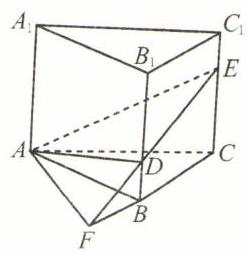
\includegraphics[width=0.2\textwidth]{bodyxb/src/bo_d20cdrf7aajc73bfmvhg_145_815_221_247_255_0.jpg}
\end{center}


(第 21 题)

\begin{center}
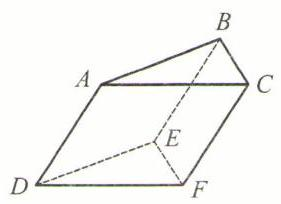
\includegraphics[width=0.2\textwidth]{bodyxb/src/bo_d20cdrf7aajc73bfmvhg_145_451_272_281_204_0.jpg}
\end{center}


(第 20 题)

\begin{center}
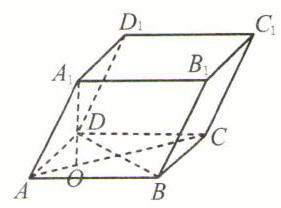
\includegraphics[width=0.2\textwidth]{bodyxb/src/bo_d20cdrf7aajc73bfmvhg_145_1155_936_281_208_0.jpg}
\end{center}


(第 23 题)

\begin{center}
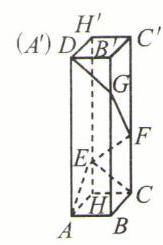
\includegraphics[width=0.2\textwidth]{bodyxb/src/bo_d20cdrf7aajc73bfmvhg_145_1270_1208_163_245_0.jpg}
\end{center}


(第 24 题)

$\therefore \;\cos {\theta }_{1} = \dfrac{{\left( \sqrt{2}a\right) }^{2} + {\left( \sqrt{2}a\right) }^{2} - {\left( \sqrt{6}a\right) }^{2}}{2 \cdot  \sqrt{2}a \cdot  \sqrt{2}a} =  - \dfrac{1}{2},$

$\therefore$ 夹角 ${\theta }_{1} = {120}^{ \circ  }$ .

(2)如图,连接 ${EC}$ ,可证 ${EC} ⫫ {A}^{\prime }G$ ,则 ${EF} = {EC} = \sqrt{2},{FC} = {2a}$ ,

$\therefore$ 异面直线 ${A}^{\prime }G$ 和 ${EF}$ 所成的角为 ${90}^{ \circ  }$ .

(3)由(2)可得, ${AE} = {EC} = {AC}$ ,

$\therefore$ 异面直线 ${A}^{\prime }G$ 和 ${AE}$ 所成的角为 ${60}^{ \circ  }$ .

25. (1) 如图,过点 $C$ 作 ${CD}\bot {AB},{CE}\bot {A{B}_{1}}$ ,连接 ${DE}$ .

\begin{center}
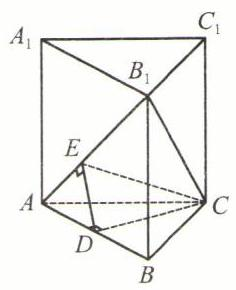
\includegraphics[width=0.2\textwidth]{bodyxb/src/bo_d20cdrf7aajc73bfmvhg_145_1203_1509_236_290_0.jpg}
\end{center}


(第 25 题)

$\because {CD} \bot  {AB},{CD} \bot  B{B}_{1}$ ,

$\therefore {CD} \bot$ 平面 $A{A}_{1}{B}_{1}B$ . 又 ${CE} \bot  A{B}_{1}$ ,

$\therefore {DE} \bot  A{B}_{1}$ .

$\therefore \angle {CED}$ 为平面 ${A}_{1}{AB}{B}_{1}$ 与平面 ${ABC}$ 所成的锐二面角,为 ${60}^{ \circ  }$ .

(2) $S = \left( {\dfrac{a}{3} + a}\right)  \cdot  \dfrac{2\sqrt{3}}{3}a \cdot  \dfrac{1}{2} = \dfrac{4}{9}\sqrt{3}{a}^{2}$ .

26. (1) 延长 ${AC}$ 至点 $D$ ,使 ${AC} = {CD}$ ,则 ${A}_{1}C//{C}_{1}D$ , $\because {B}_{1}B\bot {BD}$ , ${AB}\bot {BD}$ ,

$\therefore {BD} \bot$ 平面 ${A}_{1}{AB}{B}_{1},\;\therefore {BD} \bot  A{B}_{1}$ .

又 $B{C}_{1} \bot  A{B}_{1},\therefore A{B}_{1} \bot$ 平面 ${C}_{1}{BD},\therefore A{B}_{1} \bot  {C}_{1}D$ ,即 $A{B}_{1} \bot  {A}_{1}C$ .

(2)①作 ${EG}\bot {A}_{1}C$ 于点 $G$ ,则 ${EG}\bot$ 面 $A{C}_{1}$ ,取 ${AC}$ 的中点 $F$ . 则 ${BF}\bot {AC}$ , $\therefore {BF}\bot$ 面 $A{C}_{1}$ , $\therefore {BF}\bot {EG}$ .

$\therefore G$ 是 ${A}_{1}C$ 的中点, $\therefore {BE} = \dfrac{1}{2}B{B}_{1}$ ,即 ${BE} = E{B}_{1}$ .

② $\cos \alpha  = \dfrac{{S}_{\bigtriangleup {A}_{1}{B}_{1}{C}_{1}}}{{S}_{\bigtriangleup {A}_{1}{EC}}} = \dfrac{\sqrt{2}}{2},\;\therefore$ 锐二面角为 ${45}^{ \circ  }$ .

27. (1) $\because {BC}{C}_{1}{B}_{1}$ 为正方形, $\therefore B{C}_{1}\bot {B}_{1}C$ . 又 ${AC}\bot {BC},{AC}\bot C{C}_{1},\therefore {AC}\bot$ 平面 ${BC}{C}_{1}{B}_{1}$ ,

$\therefore {AC} \bot  B{C}_{1}$ ,且 ${B}_{1}C$ 与 ${AC}$ 相交于点 $C,\therefore B{C}_{1} \mid$ 平面 $A{B}_{1}C$ . 又 $A{B}_{1}$ 在平面 $A{B}_{1}C$ 上,

$\therefore B{C}_{1} \bot  A{B}_{1}$ ,即 $A{B}_{1}$ 与 $B{C}_{1}$ 所成角为 ${90}^{ \circ  }$ .

( 2 )如图,分别以 ${AC}$ 为底面一边作两个正方体 ${ACBD} - {A}_{1}{C}_{1}{B}_{1}{D}_{1}$ 和 ${ACFG} - {A}_{1}{C}_{1}{F}_{1}{G}_{1},B{C}_{1}//C{F}_{1}$ ,则 ${CE}$ 与 $B{C}_{1}$ 所成角为 $\angle {DC}{F}_{1}$ 或其补角. 由题可得 ${DC} = C{F}_{1} = \sqrt{2}a,D{F}_{1} = \sqrt{{a}^{2} + 4{a}^{2} + {a}^{2}} = \sqrt{6}a,\therefore \cos \angle {DC}{F}_{1} =$  $\dfrac{2{a}^{2} + 2{a}^{2} - 6{a}^{2}}{2 \cdot  \sqrt{2}a \cdot  \sqrt{2}a} =  - \dfrac{1}{2},\therefore {CE}$ 与 $B{C}_{1}$ 所成角为 ${60}^{ \circ  }$ .

(3) 如图,过点 ${C}_{1}$ 作 ${CH}\bot {A}_{1}{B}_{1}$ ,交 ${A}_{1}{B}_{1}$ 于点 $H$ ,则有 ${C}_{1}H$ 上面 ${AB}{B}_{1}{A}_{1}$ ,且 $\cos \theta  = \dfrac{{S}_{\bigtriangleup {HA}{B}_{1}}}{{S}_{\bigtriangleup {C}_{1}A{B}_{1}}} = \dfrac{\dfrac{\sqrt{2}}{2} \cdot  1}{\sqrt{2} \cdot  1} = \dfrac{1}{2},\therefore$ 二面角 ${A}_{1} - A{B}_{1} - {C}_{1}$ 的大小为 ${60}^{ \circ  }$ .

\begin{center}
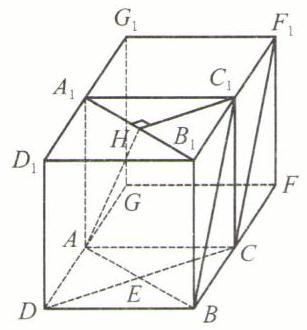
\includegraphics[width=0.2\textwidth]{bodyxb/src/bo_d20cdrf7aajc73bfmvhg_146_525_500_307_330_0.jpg}
\end{center}


(第 27 题)

\begin{center}
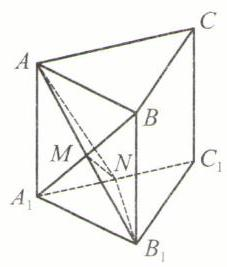
\includegraphics[width=0.2\textwidth]{bodyxb/src/bo_d20cdrf7aajc73bfmvhg_146_915_560_227_267_0.jpg}
\end{center}


(第 28 题)

28. 如图,连接 ${A}_{1}B$ 与 $A{B}_{1}$ ,交于点 $M$ . 取 ${A}_{1}{C}_{1}$ 的中点 $N$ ,连接 ${B}_{1}N$ , ${AN}$ , ${MN}$ . “ ” $M$ 为 ${A}_{1}B$ 的中点, $N$ 为 ${A}_{1}{C}_{1}$ 的中点, $\therefore {MN}//B{C}_{1},\therefore$ 转化为求截面 $A{B}_{1}N$ 与底面所成的角. $\because \Delta {A}_{1}{B}_{1}{C}_{1}$ 为正三角形, $N$ 为 ${A}_{1}{C}_{1}$ 的中点,

$\therefore {A}_{1}{C}_{1} \bot  {B}_{1}N$ . 又 ${B}_{1}N \bot  A{A}_{1},\therefore {B}_{1}N \bot$ 平面 ${AC}{C}_{1}{A}_{1},\therefore {B}_{1}N \bot  {AN}$ ,则 $\angle {AN}{A}_{1}$ 即为截面 $A{B}_{1}N$ 与底面所成的角. 在 $\operatorname{Rt}\bigtriangleup A{A}_{1}N$ 中, $A{A}_{1} = 3\sqrt{2},{A}_{1}N = \dfrac{3}{2},\therefore \tan \angle {AN}{A}_{1} = \dfrac{3\sqrt{2}}{\dfrac{3}{2}} = 2\sqrt{2}$ .

29. (1) 取 $B{C}_{1}$ 的中点 $E$ . 又 $\because D$ 为 ${AC}$ 的中点, $\therefore A{B}_{1}//{DE}$ . 又 ${DE}$ 在平面 ${DB}{C}_{1}$ 上, $\therefore A{B}_{1}//$ 平面 ${DB}{C}_{1}$ .

(2)取 ${BC}$ 的中点 $F.\because {AF}\bot {BC},\therefore {AF}\bot$ 平面 ${B}_{1}{BC}{C}_{1},\therefore A{B}_{1}$ 在侧面的射影即 $F{B}_{1}$ .

又 $\because A{B}_{1} \bot  B{C}_{1},\therefore F{B}_{1} \bot  B{C}_{1}$ ,则 $B{B}_{1} = \sqrt{2},\therefore {B}_{1}F = \sqrt{3}$ . 即射影长为 $\sqrt{3}$ .

(3)过点 $D$ 作 ${DH}\bot {BC}$ 于点 $H,\cos \theta  = \dfrac{{S}_{\bigtriangleup {C}_{1}{BH}}}{{S}_{\bigtriangleup {C}_{1}{BD}}} = \dfrac{\sqrt{2}}{2},\;\therefore \;\theta  = {45}^{ \circ  }$ .

30. D 提示:如图,在正三棱锥 $O - {ABC}$ 中,过点 $A$ 作 ${AM}\bot {BC}$ ,交 ${BC}$ 于点 $M$ ,过点 $O$ 作 ${OH}\bot$ 底面 ${ABC}$ ,交 ${AM}$ 于点 $H$ . 设棱长为 1,则 ${CM} = \dfrac{1}{2}$ ,则 ${AM} = \dfrac{\sqrt{3}}{2}$ ,则 ${AH} = \dfrac{2}{3} \cdot  \dfrac{\sqrt{3}}{2} = \dfrac{\sqrt{3}}{3}$ . 在 Rt $\bigtriangleup  {AHO}$ 中, $\cos \angle {OAH} = \dfrac{AH}{AO} = \dfrac{\dfrac{\sqrt{3}}{3}}{1} = \dfrac{\sqrt{3}}{3}$ , $\therefore$ 选 D.

\begin{center}
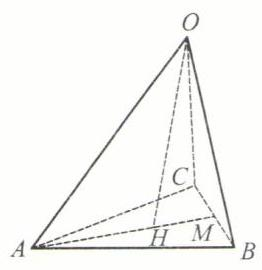
\includegraphics[width=0.2\textwidth]{bodyxb/src/bo_d20cdrf7aajc73bfmvhg_146_563_1529_262_270_0.jpg}
\end{center}


(第 30 题)

\begin{center}
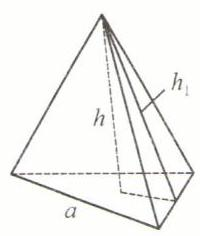
\includegraphics[width=0.2\textwidth]{bodyxb/src/bo_d20cdrf7aajc73bfmvhg_146_909_1557_200_236_0.jpg}
\end{center}


(第 31 题)

31. A 提示: 如图,设正三棱锥的底面边长为 $a$ ,斜高为 ${h}_{1}$ ,高为 $h$ . 由题意可得 $\dfrac{\dfrac{1}{2}a{h}_{1}}{\dfrac{\sqrt{3}}{4}{a}^{2}} = \dfrac{2}{3},\therefore {h}_{1} = \dfrac{\sqrt{3}}{3}a$ ,

$\therefore h = \sqrt{{h}_{1}^{2} - {\left( \dfrac{\sqrt{3}}{6}a\right) }^{2}} = \dfrac{a}{2},\therefore \dfrac{h}{{h}_{1}} = \dfrac{\sqrt{3}}{2},\therefore$ 选 A.

32. A 提示: $S = \dfrac{\sqrt{3}}{4} \cdot  {a}^{2} + \dfrac{1}{2} \cdot  {\left( \dfrac{\sqrt{2}}{2}a\right) }^{2} \cdot  3 = \dfrac{3 + \sqrt{3}}{4}{a}^{2},\;\therefore$ 选 A.

33. A 提示: 如图,记 ${PE},{PF},{FG}$ 的中点分别为 $A,B,C$ . 由题意可得 ${AB} ⫫ \dfrac{1}{2}{EF},{BC} ⫫ \dfrac{1}{2}{PG}$ , 即 ${AB} = \dfrac{a}{2},{BC} = \dfrac{b}{2}$ .

\begin{center}
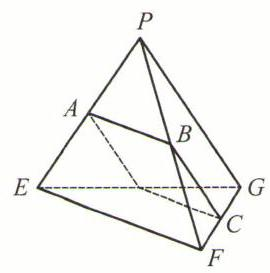
\includegraphics[width=0.2\textwidth]{bodyxb/src/bo_d20cdrf7aajc73bfmvhg_147_1163_128_270_273_0.jpg}
\end{center}


(第 33 题)

又 $\because$ 该三棱锥是正三棱锥, $\therefore {EF} \bot  {PG}$ ,即 ${AB} \bot  {BC}.\therefore$ 截面 ${ABCD}$ 为矩形,

$\therefore S = \dfrac{a}{2} \cdot  \dfrac{b}{2} = \dfrac{ab}{4},\;\therefore$ 选 A.

34. B 提示: 由题意可得 ${PD} \bot$ 底面 ${ABCD}$ ,则 $\angle {PAD} = \angle {PCD} = {45}^{ \circ  },{PB} = {15}$ . 设底面边长为 $a$ , 则 ${PD} = a,{BD} = \sqrt{2}a$ . 在 Rt $\bigtriangleup {PBD}$ 中, $P{D}^{2} + D{B}^{2} = P{B}^{2}$ ,即 ${a}^{2} + {\left( \sqrt{2}a\right) }^{2} = {15}^{2}$ , $\therefore a = 5\sqrt{3},\;\therefore$ 选 B.

\begin{center}
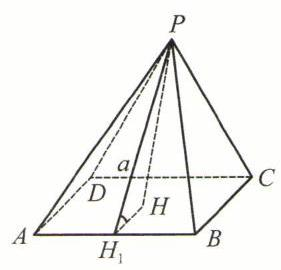
\includegraphics[width=0.2\textwidth]{bodyxb/src/bo_d20cdrf7aajc73bfmvhg_147_1152_471_281_270_0.jpg}
\end{center}


(第 35 题)

35. $C$ 提示: 如图,可得 $H{H}_{1} = \dfrac{a}{2},P{H}_{1} = \dfrac{\sqrt{3}}{2}a$ ,则在 $\mathrm{{Rt}} \bigtriangleup  {PH}{H}_{1}$ 中, $\cos \angle P{H}_{1}H = \dfrac{H{H}_{1}}{P{H}_{1}} = \dfrac{\sqrt{3}}{3}$ , $\therefore$ 选 C.

36. D 提示: ${S}_{\text{ 底 }} = {4Q}$ ,则边长为 $2\sqrt{Q},\therefore$ 选 D.

37. $C$ 提示: 由例 2 的结论, $\dfrac{{S}_{\text{ 底 }}}{{S}_{\text{ 侧 }}} = \cos {30}^{ \circ  },\;\therefore \;{S}_{\text{ 侧 }} = \dfrac{2\sqrt{3}}{3}S,\;\therefore \;$ 选 $C$ .

38. $C$ 提示: 设底面中心为 $O$ ,顶点为 $P$ ,一底边中点为 $M$ ,则 ${OM} = \sqrt{3},{PM} = \sqrt{O{M}^{2} + O{P}^{2}} =$  $2,\;\therefore \;$ 选C.

39. (1) $\sqrt{3}$ 提示:如图, ${BH} = \dfrac{\sqrt{3}}{2} \cdot  \sqrt{3} \cdot  \dfrac{2}{3} = 1$ ,又 ${PB} = 2$ ,

\begin{center}
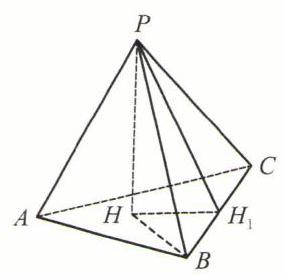
\includegraphics[width=0.2\textwidth]{bodyxb/src/bo_d20cdrf7aajc73bfmvhg_147_1151_837_284_276_0.jpg}
\end{center}


(第 39 题)

$\therefore$ 在 Rt $\bigtriangleup {PHB}$ 中, ${PH} = \sqrt{P{B}^{2} - B{H}^{2}} = \sqrt{3}$ .

(2) $2 : \sqrt{7}$ 提示:如图,设 ${PB} = {2a},{BC} = {3a}$ ,则 ${BH} = \dfrac{3a}{2} \cdot  \sqrt{3} \cdot  \dfrac{2}{3} = \sqrt{3}a$ . 又 ${PB} = {2a}$ ,

$\therefore$ 在 Rt $\bigtriangleup {PHB}$ 中, ${PH} = \sqrt{P{B}^{2} - B{H}^{2}} = a$ .

又斜高 $= \sqrt{{\left( 2a\right) }^{2} - {\left( \dfrac{3}{2}a\right) }^{2}} = \dfrac{\sqrt{7}}{2}a$ .

$\therefore \dfrac{\text{ 高 }}{\text{ 斜高 }} = \dfrac{a}{\dfrac{\sqrt{7}}{2}a} = \dfrac{2\sqrt{7}}{7}$ .

(3) $\dfrac{\sqrt{15}}{6}a$ 提示:如图, ${BH} = \dfrac{\sqrt{3}}{3}a$ ,在Rt $\bigtriangleup  {PHB}$ 中, $\angle {PBH} = {45}^{ \circ  }$ ,则 ${PB} = {BH} \cdot  \sqrt{2} = \dfrac{\sqrt{6}}{3}a$ .

$\therefore$ 斜高 $= \sqrt{P{B}^{2} - {\left( \dfrac{a}{2}\right) }^{2}} = \dfrac{\sqrt{15}}{6}a$ .

(4) $\dfrac{\sqrt{3}}{36}{a}^{2}$ 提示: 由已知,所得三角形与底面三角形相似,其边长为 $\dfrac{a}{3},\therefore S = \dfrac{1}{2} \cdot  {\left( \dfrac{1}{3}a\right) }^{2} \cdot  \sin {60}^{ \circ  } = \dfrac{\sqrt{3}}{36}{a}^{2}$ .

(5) $\dfrac{\sqrt{33}}{6}$ 提示:如图, $H{H}_{1} = \dfrac{\sqrt{3}}{3}\mathrm{\;{cm}}$ . 又 $P{H}_{1} = \sqrt{5 - 1} = 2\mathrm{\;{cm}}$ ,则在Rt $\bigtriangleup {PH}{H}_{1}$ 中, ${PH} = \sqrt{P{H}_{1}^{2} - H{H}_{1}^{2}} = \dfrac{\sqrt{33}}{3}\mathrm{\;{cm}}$ ,

$\therefore \sin \angle P{H}_{1}H = \dfrac{PH}{P{H}_{1}} = \dfrac{\sqrt{33}}{6}$ .

40. $B$ 提示: 设上、下底面三角形的高分别为 ${h}_{1},{h}_{2}$ ,则 ${h}_{1} = 2 \cdot  \dfrac{\sqrt{3}}{2} = \sqrt{3},{h}_{2} = 6 \cdot  \dfrac{\sqrt{3}}{2} = 3\sqrt{3}$ ,则 $h = \left( {\dfrac{{h}_{2}}{3} - \dfrac{{h}_{1}}{3}}\right)  \cdot  \tan {60}^{ \circ  } = \dfrac{2\sqrt{3}}{3}$  $\cdot  \sqrt{3} = 2,\;\therefore \;$ 选 B.

41. $C$ 提示: $\tan {\theta }_{1} = \dfrac{h}{\dfrac{{h}_{2}}{3} - \dfrac{{h}_{1}}{3}} = \dfrac{3h}{{h}_{2} - {h}_{1}},\tan {\theta }_{2} = \dfrac{h}{\dfrac{2{h}_{2}}{3} - \dfrac{2{h}_{1}}{3}} = \dfrac{3h}{2\left( {{h}_{2} - {h}_{1}}\right) },\;\therefore \dfrac{\tan {\theta }_{1}}{\tan {\theta }_{2}} = 2,\;\therefore$ 选 $C$ .

42. A 提示: 设上底边长为 ${2a}$ ,高为 $h$ ,则下底边长 $2 \cdot  \dfrac{\sqrt{2}a + h}{\sqrt{2}} = {2a} + \sqrt{2}h$ ,则 $\tan \theta  = \dfrac{h}{\left( {a + \dfrac{\sqrt{2}}{2}h}\right)  - a} = \sqrt{2}$ ,即 $\sin \theta  = \dfrac{\sqrt{6}}{3}$ ,

$\therefore$ 选 A.

43. D 提示: 设棱台高为 $h$ ,则由题意可得 ${\left( \dfrac{{21} - h}{21}\right) }^{2} = \dfrac{16}{49},\therefore h = 9\mathrm{\;{cm}},\therefore$ 选 D.

44. $C$ 提示:设下底面面积为 $S$ ,由题意可得 $\sqrt{64} = \dfrac{\sqrt{36} + \sqrt{S}}{2},\therefore S = {100}\left( {\mathrm{\;{cm}}}^{2}\right) \therefore$ 选 $C$ .

45. D 提示: ${h}_{\text{ 斜 }} = \dfrac{2\sqrt{3}}{3} \cdot  2 = \dfrac{4\sqrt{3}}{3},\;\therefore \;{S}_{\text{ 侧 }} = 3 \cdot  \dfrac{1}{2} \cdot  \left( {2 + 6}\right)  \cdot  \dfrac{4\sqrt{3}}{3} = {16}\sqrt{3},\;\therefore \;$ 选 D.

46. (1) 12 提示: 如图,取 ${AC}$ 中点 $M$ ,则 ${PM} = \sqrt{{13}^{2} - {5}^{2}} = {12},{MB} = \dfrac{1}{2}{AC} = 5$ ,则在 $\bigtriangleup  {PMB}$ 中, $M{B}^{2} + P{M}^{2} = P{B}^{2},\therefore {PM} \bot  {MB}$ ,即点 $P$ 到底面 ${ABC}$ 距离为 12 .

\begin{center}
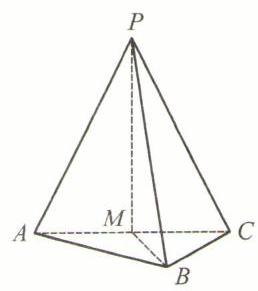
\includegraphics[width=0.2\textwidth]{bodyxb/src/bo_d20cdrf7aajc73bfmvhg_148_1248_205_258_291_0.jpg}
\end{center}


[第 46(1)题]

(2) $h\cot \beta$ 提示:过 $P$ 作 ${PO}\bot$ 底面于点 $O$ ,过点 $O$ 作 ${AB},{BC},{CA}$ 的垂线,垂足分别为 $E,F$ , $G$ . 连接 ${PE},{PF},{PG}$ . 由三垂线定理得 ${PE} \bot  {AB},{PF} \bot  {BC},{PG} \bot  {AC}$ .

$\therefore \angle {PEO},\angle {PFO},\angle {PGO}$ 分别为侧面与底面所成二面角的平面角,则 $\angle {PEO} = \angle {PFO}$  $= \angle {PGO} = \beta$ .

在 $\bigtriangleup {POE}$ 与 $\bigtriangleup {POF}$ 中, $\because {PO} \bot$ 平面 ${ABC},\therefore {PO} \bot  {OE},{PO} \bot  {OF}$ .

又 $\because {PO} = {PO},\angle {PEO} = \angle {PFO},\therefore \bigtriangleup {PEO} \cong  \bigtriangleup {PFO}$ ,

$\therefore {OE} = {OF}$ . 同理 ${OE} = {OG},\therefore {OE} = {OF} = {OG}$ . 又 $\because {OE} \bot  {AB},{OF} \bot  {BC},{OG} \bot  {AC},\therefore O$ 是 $\bigtriangleup  {AB}$

切圆的圆心. 在Rt $\bigtriangleup {PEO}$ 中, ${PO} = h,\angle {PEO} = \beta ,\therefore {OE} = h \cdot  \cot \beta$ ,即底面内切圆半径为 $h \cdot  \cot \beta$ .

(3) $\dfrac{1}{3}$ 提示:如图,取 ${EF}$ 中点 $M$ ,则 ${PM} = \dfrac{\sqrt{2}}{2} \cdot  \dfrac{1}{2} = \dfrac{\sqrt{2}}{4}$ , ${AM} = \sqrt{1 + \dfrac{1}{8}} = \dfrac{3}{4}\sqrt{2}$ ,

\begin{center}
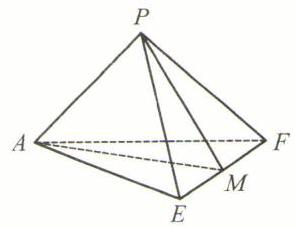
\includegraphics[width=0.2\textwidth]{bodyxb/src/bo_d20cdrf7aajc73bfmvhg_148_1214_638_295_228_0.jpg}
\end{center}


[第 46(3)题]

则 $\dfrac{3}{4}\sqrt{2} \cdot  h = 1 \cdot  \dfrac{\sqrt{2}}{4},\;\therefore \;h = \dfrac{1}{3}$ .

(4) ${24}\sqrt{5}$ 提示: $\dfrac{{S}_{\text{ 底 }}}{\cos {60}^{ \circ  }} = {S}_{\text{ 侧 }}$ ,且三角形 ${ABC}$ 三边长为 7,8,9.

$\therefore \;{S}_{\text{ 底 }} = {12}\sqrt{5},\;\therefore \;{S}_{\text{ 侧 }} = \dfrac{{12}\sqrt{5}}{\dfrac{1}{2}} = {24}\sqrt{5}$ .

47. (1) $\dfrac{\sqrt{5}}{5}$ 提示:如图, ${PB} \bot$ 底面 ${ABCD}$ , $\therefore {PB} \bot  {AD}$ ,又 ${DA} \bot  {AB}$ , $\therefore {DA} \bot$ 平面 ${PAB}$ . 在Rt $\bigtriangleup  {PBA}$ 中, ${AB} = 1$ , ${PB} = \sqrt{3},\therefore {PA} = 2$ ,在Rt $\bigtriangleup  {PAD}$ 中, ${AD} = 1,{AP} = 2,\therefore {DP} = \sqrt{5},\therefore \cos \angle {APD} = \dfrac{AD}{DP} = \dfrac{1}{\sqrt{5}} = \dfrac{\sqrt{5}}{5}$ .

\begin{center}
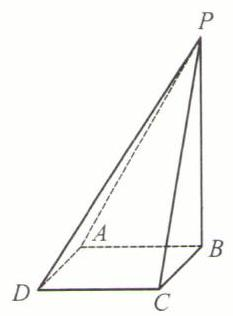
\includegraphics[width=0.2\textwidth]{bodyxb/src/bo_d20cdrf7aajc73bfmvhg_148_562_1134_233_316_0.jpg}
\end{center}


[第 47(1)题]

\begin{center}
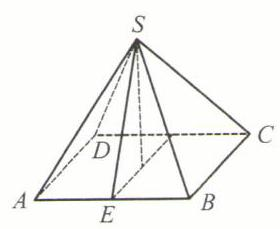
\includegraphics[width=0.2\textwidth]{bodyxb/src/bo_d20cdrf7aajc73bfmvhg_148_875_1220_280_229_0.jpg}
\end{center}


[第 47(2)题]

(2) $\dfrac{Q}{P}$ 提示:如图,过点 $S$ 作 ${SE}\bot {AB}$ 于点 $E$ . 设 ${SE} = h$ ,又底面边长为 $\sqrt{Q}$ ,且 ${S}_{SAB} = \dfrac{P}{4}$ ,

$\therefore h = \dfrac{P}{2\sqrt{Q}}$ ,则 $\cos \alpha  = \dfrac{\dfrac{\sqrt{Q}}{2}}{h} = \dfrac{\dfrac{\sqrt{Q}}{2}}{\dfrac{P}{2\sqrt{Q}}} = \dfrac{Q}{P}$ .

\begin{center}
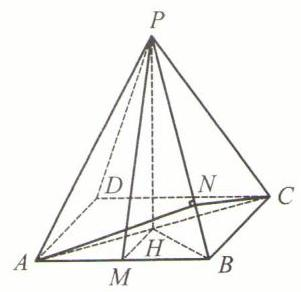
\includegraphics[width=0.2\textwidth]{bodyxb/src/bo_d20cdrf7aajc73bfmvhg_148_1215_1571_301_292_0.jpg}
\end{center}


[第 47(3)题]

(3) $- \dfrac{1}{7}$ 提示:如图, ${PH} \bot$ 底面 ${ABCD}$ , ${PM} \bot  {AB}$ . 设底面边长为 $a$ ,则 ${BH} = \dfrac{\sqrt{2}}{2}a$ ,在 $\mathrm{{Rt}} \bigtriangleup  {PHB}$ 中, $\angle {PBH} = {60}^{ \circ  }$ , $\therefore {PB} = \sqrt{2}a$ . 在 Rt $\bigtriangleup  {PMB}$ 中, ${PB} = \sqrt{2}a,{MB} = \dfrac{a}{2}$ . $\therefore {PM} = \sqrt{P{B}^{2} - B{M}^{2}} = \dfrac{\sqrt{7}}{2}a$ . 过点 $A$ 作 ${AN} \bot  {PB}$ 于点 $N$ ,连接 ${CN}$ . $\because \bigtriangleup {PAB}$  $\cong  \bigtriangleup {PCB},\therefore {CN} \bot  {PB}$ . 在 $\bigtriangleup {ANC}$ 中, ${AN} = {NC} = \dfrac{{AB} \cdot  {PM}}{PB} = \dfrac{\sqrt{14}}{4}a$ ,且 ${AC} = \sqrt{2}a$ .

$\therefore \cos \angle {ANC} = \dfrac{A{N}^{2} + C{N}^{2} - A{C}^{2}}{2 \cdot  {AN} \cdot  {CN}} = \dfrac{{\left( \dfrac{\sqrt{14}}{4}a\right) }^{2} + {\left( \dfrac{\sqrt{14}}{4}a\right) }^{2} - {\left( \sqrt{2}a\right) }^{2}}{2 \cdot  \dfrac{\sqrt{14}}{4}a \cdot  \dfrac{\sqrt{14}}{4}a} =  - \dfrac{1}{7}$ .

48. (1) $\dfrac{50}{3}\dfrac{40}{3}$ 提示: ${S}_{\text{ 梯 }} = \dfrac{{S}_{\text{ 侧 }}}{4} = \dfrac{{20}^{2} + {40}^{2}}{4} = {500}$ ,又 ${S}_{\text{ 梯 }} = \dfrac{1}{2} \cdot  \left( {{20} + {40}}\right)  \cdot  {h}_{\text{ 斜高 }},\therefore {h}_{\text{ 斜高 }} = \dfrac{500}{\dfrac{1}{2}\left( {{20} + {40}}\right) } = \dfrac{50}{3}\left( \mathrm{\;{cm}}\right)$ ,

$\therefore h = \sqrt{{h}_{\text{ 斜高 }}^{2} - {\left( \dfrac{{40} - {20}}{2}\right) }^{2}} = \dfrac{40}{3}\left( \mathrm{\;{cm}}\right)$ .

(2) $3\sqrt{3}\left( {{b}^{2} - {a}^{2}}\right)$ 提示: ${h}_{\text{ 斜 }} = \left( {\dfrac{\sqrt{3}}{2}b - \dfrac{\sqrt{3}}{2}a}\right)  \cdot  \dfrac{1}{\cos {60}^{ \circ  }} = \sqrt{3}\left( {b - a}\right) ,\;\therefore \;{S}_{\text{ 侧 }} = 6 \cdot  \dfrac{1}{2} \cdot  \left( {a + b}\right)  \cdot  {h}_{\text{ 斜 }} = 6 \cdot  \dfrac{1}{2} \cdot  \left( {a + b}\right)$  $\cdot  \sqrt{3}\left( {b - a}\right)  = 3\sqrt{3}\left( {{b}^{2} - {a}^{2}}\right) .$

(3)364 提示: ${h}_{\text{ 斜 }} = \sqrt{{12}^{2} + {5}^{2}} = {13}$ (cm). 又 ${a}^{2} + {b}^{2} + 4 \cdot  \dfrac{1}{2} \cdot  \left( {a + b}\right)  \cdot  {13} = {512}$ ,

$\therefore \;{a}^{2} + {b}^{2} + {26}\left( {a + b}\right)  = {512},\;\therefore \;{a}^{2} + {\left( a + {10}\right) }^{2} + {26}\left( {a + a + {10}}\right)  = {512}$ ,

$\therefore {a}^{2} + {36a} - {76} = 0$ ,即 $\left( {a - 2}\right) \left( {a + {38}}\right)  = 0$ ,解得 $a = 2$ (负根舍去) $\therefore {S}_{\text{ 侧 }} = 4 \cdot  \dfrac{1}{2} \cdot  \left( {2 + 2 + {10}}\right)  \cdot  {13} = {364}\left( {\mathrm{\;{cm}}}^{2}\right)$ .

49. (1) $\dfrac{1}{2}$ 提示: 如图, $\angle {AMH} = {45}^{ \circ  }$ ,设高 ${AH} = h$ ,则 ${HM} = h$ .

$\because$ 底面为正三角形, $\therefore {CH} = {2HM} = {2h}$ . 在 Rt $\bigtriangleup {AHC}$ 中, $\tan \theta  = \tan \angle {ACH} = \dfrac{AH}{CH} = \dfrac{h}{2h} = \dfrac{1}{2}$ .

(2) $\dfrac{\sqrt{5}}{5}$ 提示:如图, $\angle {ACH} = {45}^{ \circ  }$ ,设高 ${AH} = h$ ,则 ${CH} = h$ .

$\because$ 底面为正三角形, $\therefore {HM} = \dfrac{CH}{2} = \dfrac{h}{2}$ . 在 Rt $\bigtriangleup  {AHM}$ 中, $\cos \angle {AMH} = \dfrac{HM}{AM} = \dfrac{\dfrac{h}{2}}{\sqrt{{\left( \dfrac{h}{2}\right) }^{2} + {h}^{2}}} = \dfrac{\sqrt{5}}{5}$ .

\begin{center}
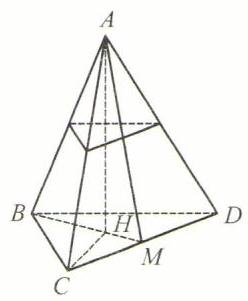
\includegraphics[width=0.2\textwidth]{bodyxb/src/bo_d20cdrf7aajc73bfmvhg_149_293_983_248_301_0.jpg}
\end{center}


[第 49(1)题]

\begin{center}
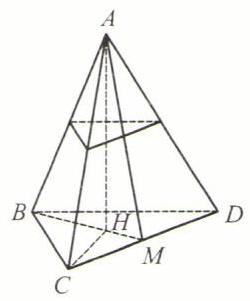
\includegraphics[width=0.2\textwidth]{bodyxb/src/bo_d20cdrf7aajc73bfmvhg_149_625_983_250_301_0.jpg}
\end{center}


[第 49(2)题]

\begin{center}
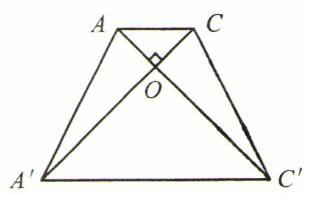
\includegraphics[width=0.2\textwidth]{bodyxb/src/bo_d20cdrf7aajc73bfmvhg_149_960_1087_309_197_0.jpg}
\end{center}


[第 49(3)题]

(3)96 提示:如图, ${AC} = 2\sqrt{2},{A}^{\prime }{C}^{\prime } = 6\sqrt{2}$ ,且 $A{C}^{\prime }\bot {A}^{\prime }C$ . 四边形 ${AC}{C}^{\prime }{A}^{\prime }$ 为等腰梯形.

$\therefore {AO} = {CO} = 2,{A}^{\prime }O = {C}^{\prime }O = 6$ . 则 ${A}^{\prime }A = {C}^{\prime }C = \sqrt{{6}^{2} + {2}^{2}} = 2\sqrt{10}$ ,则 ${h}_{\text{ 斜 }} = \sqrt{{\left( 2\sqrt{10}\right) }^{2} - {\left( 3 - 1\right) }^{2}} = 6$ ,

$\therefore \;{S}_{\text{ 侧 }} = 4 \cdot  \dfrac{1}{2} \cdot  \left( {6 + 2}\right)  \cdot  6 = {96}.$

\begin{center}
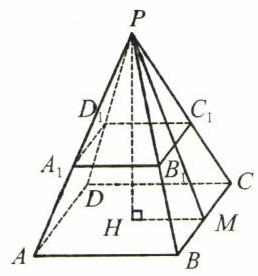
\includegraphics[width=0.2\textwidth]{bodyxb/src/bo_d20cdrf7aajc73bfmvhg_149_1175_1447_258_276_0.jpg}
\end{center}


[第 50(1)题]

50. (1) $\left( {5 + 3\sqrt{2}}\right) {a}^{2}$ 提示: 由题意可知棱台上底面边长 ${A}_{1}{B}_{1} = a$ ,在 Rt $\bigtriangleup  {PHM}$ 中, ${HM} = a$ , $\angle {PMH} = {45}^{ \circ  }$ ,

$\therefore {PM} = \sqrt{2}a$ ,则 ${S}_{B{B}_{1}{C}_{1}C} = \dfrac{3}{4} \cdot  {S}_{\bigtriangleup {PBC}} = \dfrac{3}{4} \cdot  \dfrac{1}{2} \cdot  {BC} \cdot  {PM} = \dfrac{3}{4} \cdot  \dfrac{1}{2} \cdot  {2a} \cdot  \sqrt{2}a =$  $\dfrac{3\sqrt{2}}{4}{a}^{2}$ .

$\therefore \;{S}_{\text{ 表 }} = 4{S}_{B{B}_{1}{C}_{1}C} + {S}_{{A}_{1}{B}_{1}{C}_{1}{D}_{1}} + {S}_{ABCD} = 3\sqrt{2}{a}^{2} + {a}^{2} + 4{a}^{2} = \left( {3\sqrt{2} + 5}\right) {a}^{2}$ .

(2) $\dfrac{8}{9}Q$ 提示: $\dfrac{{S}_{\text{ 小侧 }}}{{S}_{\text{ 锥侧 }}} = {\left( \dfrac{PA}{PO}\right) }^{2},\therefore {S}_{\text{ 小侧 }} = \dfrac{Q}{9}$ ,得 ${S}_{\text{ 台側 }} = {S}_{\text{ 锥侧 }} - {S}_{\text{ 小侧 }} = \dfrac{8}{9}Q$ .

(3) $1 : 3 : 5$ 提示: ${S}_{1} : {S}_{2} : {S}_{3} = {1}^{2} : {2}^{2} : {3}^{2} = 1 : 4 : 9,\therefore {S}_{1} : \left( {{S}_{2} - {S}_{1}}\right)  : \left( {{S}_{3} - {S}_{2}}\right)  : 1 : 3 : 5$ .

4) $\left( {Q - \sqrt{Q{Q}^{\prime }}}\right)  : Q$ 提示: 设棱台高为 ${h}^{\prime }$ ,原棱锥高为 $h$ . 则 ${\left( \dfrac{h - {h}^{\prime }}{h}\right) }^{2} = \dfrac{{Q}^{\prime }}{Q} \Rightarrow  \dfrac{h - {h}^{\prime }}{h} = \sqrt{\dfrac{{Q}^{\prime }}{Q}} \Rightarrow  \dfrac{{h}^{\prime }}{h} = 1 - \sqrt{\dfrac{{Q}^{\prime }}{Q}}$  $= \dfrac{Q - \sqrt{Q{Q}^{\prime }}}{Q}$ .

(5) $2 : 1$ 提示: 设所求之比为 $\dfrac{n}{m}$ ,则 $\sqrt{25} = \dfrac{m \cdot  \sqrt{1} + n \cdot  \sqrt{49}}{m + n},\therefore \dfrac{m}{n} = \dfrac{1}{2},\therefore$ 截面到上、下底面的距离之比为 2 .

51. (1)如图,取 ${BD}$ 的中点 $M$ , $\because M$ 为菱形中心, $\therefore {AM}\bot {BD}$ . 又 $\because {PA}\bot$ 平面 ${ABCD}$ ,由三垂线定理得 ${PM}\bot {BD},\therefore \angle {PMA}$ 为二面角 $P - {BD} - A$ 的平面角.

\begin{center}
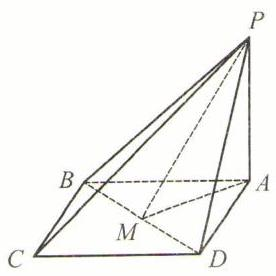
\includegraphics[width=0.2\textwidth]{bodyxb/src/bo_d20cdrf7aajc73bfmvhg_150_1236_121_276_276_0.jpg}
\end{center}


(第 51 题)

$\because {ABCD}$ 是边长为 ${2a}$ 的菱形, $\therefore {AB} = {AD}$ .

又 $\because \angle {BAD} = {60}^{ \circ  },\therefore \bigtriangleup {ABD}$ 为等边三角形,

$\therefore {AM} = {2a}\cos {30}^{ \circ  } = \sqrt{3}a$ . 在 Rt $\bigtriangleup  {PAM}$ 中, ${PA} = \sqrt{3}a$ ,

$\therefore \tan \angle {PMA} = \dfrac{PA}{AM} = 1,\;\therefore \;$ 二面角 $P - {BD} - A$ 为 ${45}^{ \circ  }$ ,

$\therefore$ 平面 ${PBD}$ 与底面 ${ABCD}$ 所成锐二面角为 ${45}^{ \circ  }$ .

(2)设 $A$ 到平面 ${PBD}$ 的距离为 $h.\because {V}_{A - {BDP}} = {V}_{P - {ABD}},\therefore {S}_{\bigtriangleup {ABD}} \cdot  {PA} \cdot  \dfrac{1}{3} = {S}_{\bigtriangleup {PBD}}$ .

$h \cdot  \dfrac{1}{3}$ . 又 ${S}_{\bigtriangleup {ABD}} = \dfrac{\sqrt{3}}{4} \cdot  {\left( 2a\right) }^{2} = \sqrt{3}{a}^{2},{PA} = \sqrt{3}a,\because {AB} = {AD}$ ,且 ${PA} \bot$ 平面 ${ABCD}$ ,

$\therefore \;{PB} = {PD} = \sqrt{{\left( \sqrt{3}a\right) }^{2} + {\left( 2a\right) }^{2}} = \sqrt{7}a,$

$\therefore {PM} = \sqrt{P{D}^{2} - D{M}^{2}} = \sqrt{6}a,\;\therefore \;{S}_{\bigtriangleup {PBD}} = \dfrac{1}{2} \cdot  {BD} \cdot  {PM} = \sqrt{6}{a}^{2}$ ,则 $h = \dfrac{{S}_{\bigtriangleup {ABD}} \cdot  {PA}}{{S}_{\bigtriangleup {PBD}}} = \dfrac{\sqrt{3}{a}^{2} \cdot  \sqrt{3}a}{\sqrt{6}{a}^{2}} = \dfrac{\sqrt{6}}{2}a$ .

52. (1) 设棱锥高为 $x$ ,则 $\dfrac{150}{54} = {\left( \dfrac{x}{x - {14}}\right) }^{2}$ ,即 $\dfrac{x}{x - {14}} = \dfrac{5}{3}$ ,解得 $x = {35},\therefore$ 棱锥高为 ${35}\mathrm{\;{cm}}$ .

(2)设 ${SO}$ 为棱锥的高,它与截面交于点 ${O}_{1},\because {AB} = 8\mathrm{\;{cm}}$ ,且 ${ABCDEF}$ 为正六边形,

$\therefore {AO} = {AB} = 8\mathrm{\;{cm}}$ . 又 ${SA} = {10}\mathrm{\;{cm}},\therefore {SO} = 6\mathrm{\;{cm}}$ .

$\because \;{S}_{\text{ 底 }} = \dfrac{\sqrt{3}}{4} \cdot  {8}^{2} \cdot  6 = {96}\sqrt{3}\left( {\mathrm{\;{cm}}}^{2}\right)$ ,又 ${S}_{\text{ 截 }} = \dfrac{32}{3}\sqrt{3}{\mathrm{\;{cm}}}^{2}$ ,且 $\dfrac{{S}_{\text{ 裁 }}}{{S}_{\text{ 底 }}} = \dfrac{S{O}_{1}^{2}}{{6}^{2}},\;\therefore \;S{O}_{1} = 2\left( \mathrm{\;{cm}}\right)$ .

$\therefore {SO} - S{O}_{1} = 6 - 2 = 4\left( \mathrm{\;{cm}}\right)$ . 即截面与底面相距 $4\mathrm{\;{cm}}$ .

53. D 提示:如图, ${BC}\bot {CD},{AB}\bot$ 平面 ${BCD}$ ,则 ${CD}\bot$ 平面 ${ABC}$ , $\therefore {CD}\bot {AC}$ ,

$\therefore$ 三个侧面都是直角三角形 $\therefore$ 选 D.

\begin{center}
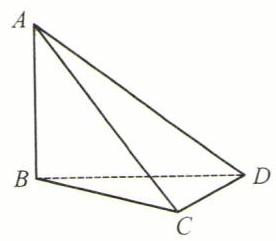
\includegraphics[width=0.2\textwidth]{bodyxb/src/bo_d20cdrf7aajc73bfmvhg_150_522_1123_276_241_0.jpg}
\end{center}


(第 53 题)

\begin{center}
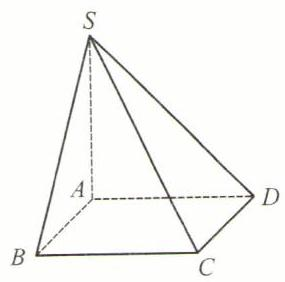
\includegraphics[width=0.2\textwidth]{bodyxb/src/bo_d20cdrf7aajc73bfmvhg_150_884_1075_285_282_0.jpg}
\end{center}


(第 54 题)

54. A 提示:如图,当底面 ${ABCD}$ 为正方形, ${SA} \bot$ 底面 ${ABCD}$ 时,四个侧面均为直角三角形. $\therefore$ 选 A.

55. B 提示: 根据正四棱锥侧面积是底面积的 2 倍,不妨令 $P$ 为顶点,底面为 ${ABCD},Q$ 为 ${AB}$ 的中点, $O$ 为底面中心,则 ${PQ}$  $= 2 \cdot  {OQ}.\because {PQ} \bot  {AB},\therefore {OQ} \bot  {AB}.\therefore \angle {PQO}$ 即为侧面与底面所成角.

\begin{center}
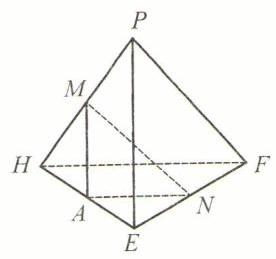
\includegraphics[width=0.2\textwidth]{bodyxb/src/bo_d20cdrf7aajc73bfmvhg_150_1256_1537_276_259_0.jpg}
\end{center}


(第 56 题)

$\because \cos \angle {PQO} = \dfrac{OQ}{PQ} = \dfrac{1}{2},\therefore$ 选 B.

56. C 提示: 如图,取 ${HE}$ 的中点 $A$ ,则 $\angle {AMN}$ 为异面直线 ${MN}$ 与 ${PE}$ 所成角或其补角. 不妨设棱长为 2,则 ${AM} = 1,{AN} = 1$ .

$\because {PE} \bot  {HF},\therefore {MA} \bot  {HF},\therefore \angle {AMN} = {45}^{ \circ  },\therefore$ 选 C.

57. $D$ 提示: ${\left( \dfrac{{h}_{ \pm  }}{{h}_{ \pm  }}\right) }^{2} = \dfrac{1}{2} \Rightarrow  \dfrac{{h}_{ \pm  }}{{h}_{ \pm  }} = \dfrac{1}{\sqrt{2}} \Rightarrow  \dfrac{{h}_{ \pm  }}{{h}_{ \pm  } - {h}_{ \pm  }} = \dfrac{1}{\sqrt{2} - 1}$ ,即 $\dfrac{{h}_{ \pm  }}{{h}_{ \mp  }} = \dfrac{1}{\sqrt{2} - 1},\;\therefore$ 选 $D$ .

58. D 提示: ${\left( \dfrac{{h}_{ \pm  }}{{h}_{ \pm  }}\right) }^{2} = \dfrac{1}{\sqrt{2}} \Rightarrow  \dfrac{{h}_{ \pm  }}{{h}_{ \pm  }} = \dfrac{1}{\sqrt[4]{2}} \Rightarrow  \dfrac{{h}_{ \pm  }}{{h}_{ \pm  } - {h}_{ \pm  }} = \dfrac{1}{\sqrt[4]{2} - 1}$ ,即 $\dfrac{{h}_{ \pm  }}{{h}_{ \mp  }} = \dfrac{1}{\sqrt[4]{2} - 1},\therefore$ 选 D.

\begin{center}
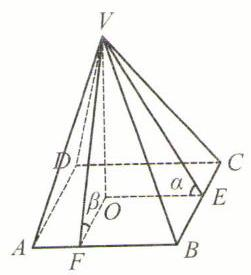
\includegraphics[width=0.2\textwidth]{bodyxb/src/bo_d20cdrf7aajc73bfmvhg_150_1288_1844_251_275_0.jpg}
\end{center}


(第 60 题)

59. C 提示: $\because {h}_{1} : \left( {{h}_{1} + {h}_{2}}\right)  : \left( {{h}_{1} + {h}_{2} + {h}_{3}}\right)  = 1 : \sqrt{2} : \sqrt{3}$ ,

$\therefore {h}_{1} : {h}_{2} : {h}_{3} = 1 : \left( {\sqrt{2} - 1}\right)  : \left( {\sqrt{3} - \sqrt{2}}\right) ,\;\therefore$ 选 C.

60. C 提示: 如图,设侧面 ${VBC}$ 与底面所成角为 $\alpha$ ,侧面 ${VAB}$ 与底面所成角为 $\beta$ ,则 $\alpha  = \beta$ . 在 $\mathrm{{Rt}} \bigtriangleup  {VOE}$ 中, ${OE} = {VO} \cdot  \cot \alpha$ . 在 $\mathrm{{Rt}} \bigtriangleup  {VOF}$ 中, ${OF} = {VO} \cdot  \cot \beta ,{OE} = {OF},{BC}\bot {OE},{AB}\bot {OF}$ ,

$\therefore$ 以 $O$ 为圆心以 ${OE}$ 为半径的圆与 ${BC},{AB}$ 相切. 同理,此圆也与边 ${DC},{AD}$ 相切,

$\therefore$ 底面四边形必是圆外切四边形, $\therefore$ 选 C.

61. D 提示:若为正六棱锥,则底面为正六边形. 由 6 个等边三角形构成,设边长为 $r$ ,正六棱锥的高为 $h$ ,侧棱长为 $l$ . 则由 ${h}^{2} + {r}^{2} = {l}^{2}$ ,且 $h \neq  0$ ,得 $r \neq  l,\therefore$ 不可能为正六棱锥, $\therefore$ 选 D.

62. $B$ 提示:设斜高为 ${h}^{\prime }$ ,高为 $h$ ,则 ${h}^{\prime } = \sqrt{{h}^{2} + {\left( \dfrac{\sqrt{3}}{2}a\right) }^{2}} = \sqrt{{h}^{2} + \dfrac{3}{4}{a}^{2}},\;\therefore \;{S}_{\text{ 侧 }} = \dfrac{1}{2}a{h}^{\prime } \cdot  6 = {3a}\sqrt{{h}^{2} + \dfrac{3}{4}{a}^{2}} =$  $\dfrac{3a}{2}\sqrt{4{h}^{2} + 3{a}^{2}},\;\therefore \;$ 选 B.

63. D 提示:由题可得侧棱相等,侧面是全等的等腰直角三角形, $\therefore$ 底面是等边三角形,

$\therefore$ 三棱锥为正三棱锥, $\therefore$ 顶点在底面射影为底面中心, $\therefore$ 选 D.

64. B 提示: 如图,以面 ${SAB}$ 与面 ${SAD}$ 为例. 作 ${BP} \bot  {SA}$ 于点 $P$ ,则 ${DP} \bot  {SA}$ 于点 $P$ ,此时面 ${SAB}$ 与面 ${SAD}$ 所成的二面角为 $\angle {BPD}.\bigtriangleup {PAB}$ 中, ${AB}$ 是斜边, ${PB}$ 是直角边,必有 ${AB} > {PB}$ . 同理 ${AD} > {PD},\bigtriangleup {ABD}$ 为等腰直角三角形, $\angle {BAD}$  $= {90}^{ \circ  }$ , $\therefore  \bigtriangleup  {PBD}$ 为等腰三角形, ${PB} = {PD}$ 小于 ${AB} = {AD}$ . 由余弦定理, $\angle {BPD} > \angle {BAD}$ ,必为钝角, $\therefore$ 选 B.

\begin{center}
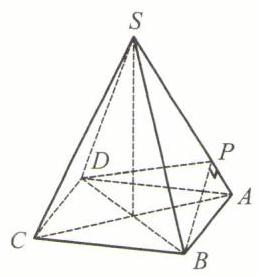
\includegraphics[width=0.2\textwidth]{bodyxb/src/bo_d20cdrf7aajc73bfmvhg_151_487_509_259_276_0.jpg}
\end{center}


(第 64 题)

\begin{center}
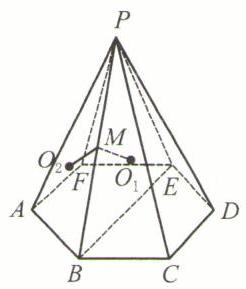
\includegraphics[width=0.2\textwidth]{bodyxb/src/bo_d20cdrf7aajc73bfmvhg_151_830_496_246_289_0.jpg}
\end{center}


(第 65 题)

65. D 提示: 如图,取 ${PB}$ 的中点 $M$ ,连接 $M{O}_{1},M{O}_{2}.\because {O}_{1}$ 是 $\bigtriangleup {BPE}$ 的外心, ${O}_{2}$ 是 $\bigtriangleup {APB}$ 的外心, $\therefore {PB} \bot  {O}_{1}M$ 且 ${PB} \bot  {O}_{2}M,\therefore {PB} \bot$ 平面 ${O}_{1}M{O}_{2},\therefore {PB} \bot  {O}_{1}{O}_{2}$ . 易证, ${AB} \bot$ 面 $P{O}_{1}{O}_{2}$ ,可得 ${AB} \bot  {O}_{1}{O}_{2},\therefore {O}_{1}{O}_{2} \bot$ 平面 ${PAB},\therefore {O}_{1}{O}_{2}$ 与侧面 ${APB}$ 所成的角为 ${90}^{ \circ  },\therefore$ 选 D.

66. D 提示:如图 1, $\bigtriangleup {ABC}$ 为 $\mathrm{{Rt}}\bigtriangleup ,\angle {BAC} = {90}^{ \circ  },{SA} \bot$ 底面 ${ABC}$ ,且 ${BA} = {SA} = {AC}$ ,则 ${SB} = {SC}$ ,满足题意, $\therefore$ 选项 (A) 错,选项 (C) 错.

如图 2, $a,b,c$ 互不相等 $\therefore$ 选项 (B) 错, $\therefore$ 选 D.

\begin{center}
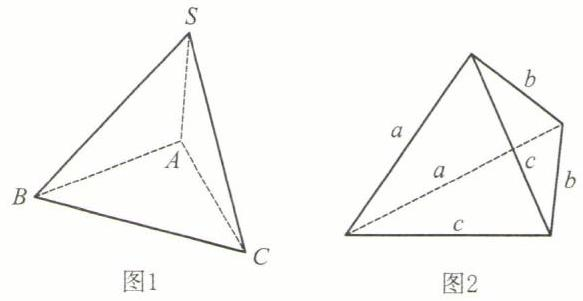
\includegraphics[width=0.4\textwidth]{bodyxb/src/bo_d20cdrf7aajc73bfmvhg_151_313_1069_583_301_0.jpg}
\end{center}


(第 66 题)

\begin{center}
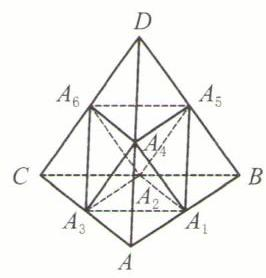
\includegraphics[width=0.2\textwidth]{bodyxb/src/bo_d20cdrf7aajc73bfmvhg_151_976_1093_266_278_0.jpg}
\end{center}


(第 67 题)

67. C 提示: 如图,在四面体 ${ABCD}$ 中, ${A}_{1},{A}_{2},{A}_{3},{A}_{4},{A}_{5},{A}_{6}$ 依次是 ${AB},{BC},{CA},{DA},{DB},{DC}$ 的中点,则由四个中截面获得一个八面体. ${S}_{\bigtriangleup {A}_{1}{A}_{2}{A}_{3}} = \dfrac{1}{4}{S}_{\bigtriangleup {ABC}},{S}_{\bigtriangleup {A}_{4}{A}_{5}{A}_{6}} = \dfrac{1}{4}{S}_{\bigtriangleup {ABC}}$ . 同理 ${S}_{\text{ 剩 }} : {S}_{\text{ 原 }} = 1 : 2,\therefore$ 选 C.

68. (1)① $\dfrac{\sqrt{2}}{3}$ ② $\dfrac{\sqrt{3}}{6}$ 提示:①如图,设 $A$ 在底面的射影为 $H$ ,则 ${AD}$ 在底面的射影为 ${HD}$ , $E$ 在底面的射影落在 ${HD}$ 上,设为 $M$ . 不妨设棱长为 1, ${AH} = \dfrac{\sqrt{6}}{3},{EM} = \dfrac{\sqrt{6}}{6}$ . 在 Rt $\bigtriangleup  {EMC}$ 中, ${EM} = \dfrac{\sqrt{6}}{6},{CE} = \dfrac{\sqrt{3}}{2},\therefore \sin \angle {ECM} = \dfrac{\dfrac{\sqrt{6}}{6}}{\dfrac{\sqrt{3}}{2}} = \dfrac{\sqrt{2}}{3}$ ,即 ${CE}$ 与底面 ${BCD}$ 所成角的正弦值为 $\dfrac{\sqrt{2}}{3}$ .

\begin{center}
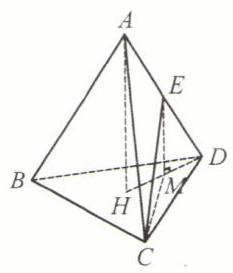
\includegraphics[width=0.2\textwidth]{bodyxb/src/bo_d20cdrf7aajc73bfmvhg_151_565_1828_233_273_0.jpg}
\end{center}


[第 68(1)①题]

\begin{center}
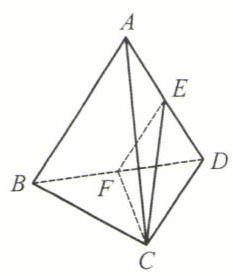
\includegraphics[width=0.2\textwidth]{bodyxb/src/bo_d20cdrf7aajc73bfmvhg_151_857_1824_233_276_0.jpg}
\end{center}


[第 68(1)②题]

②如图,取 ${BD}$ 中点 $F$ ,连接 ${CF}$ , ${EF}$ ,则 ${EF} = \dfrac{1}{2}$ , ${CE} = \dfrac{\sqrt{3}}{2}$ , ${CF} = \dfrac{\sqrt{3}}{2}$ , ${CE}$ 与 ${AB}$ 所成角即 $\angle {CEF}$ 或其补角,

$\therefore \cos \angle {CEF} = \dfrac{C{E}^{2} + E{F}^{2} - C{F}^{2}}{{2CE} \cdot  {EF}} = \dfrac{\sqrt{3}}{6}$ ,即 ${CE}$ 和 ${AB}$ 所成角的余弦值为 $\dfrac{\sqrt{3}}{6}$ . (2)① $\dfrac{2\sqrt{7}}{7}$ ② $\dfrac{\sqrt{15}}{6}$ 提示:①如图,连接 ${CD}$ ,取 ${CD}$ 的中点 $M$ ,连接 ${EM}$ , ${BM}$ , $\because$ 正三棱锥 $P - {ABC}$ 中底面边长为 1,侧棱 ${PA} = \sqrt{2},D,E$ 为 ${AB},{PC}$ 中点, $\therefore {EM}//{PD},\therefore \angle {BEM}$ 即平面直线 ${PD},{BE}$ 所成角或其补角.

由题可得 ${PD} = \sqrt{2 - \dfrac{1}{4}} = \dfrac{\sqrt{7}}{2},{CD} = \sqrt{1 - \dfrac{1}{4}} = \dfrac{\sqrt{3}}{2},\therefore {EM} = \dfrac{1}{2}{PD} = \dfrac{\sqrt{7}}{4}$ . 又 $\dfrac{2 + 2 - 1}{2 \cdot  \sqrt{2} \cdot  \sqrt{2}} = \cos \angle {BPE} = \dfrac{2 + \dfrac{1}{2} - B{E}^{2}}{2 \cdot  \sqrt{2} \cdot  \dfrac{\sqrt{2}}{2}},\therefore {BE} = 1,{BM} = \sqrt{B{D}^{2} + {\left( \dfrac{CD}{2}\right) }^{2}} = \sqrt{\dfrac{1}{4} + \dfrac{3}{16}} = \dfrac{\sqrt{7}}{4}$ .

$\therefore \cos \angle {BEM} = \dfrac{B{E}^{2} + M{E}^{2} - B{M}^{2}}{2 \cdot  {BE} \cdot  {EM}} = \dfrac{2\sqrt{7}}{7}$ ,即异面直线 ${PD}$ 与 ${BE}$ 所成角的余弦值为 $\dfrac{2\sqrt{7}}{7}$ .

②如图,过点 $P$ 作 ${PO} \bot$ 平面 ${ABC}$ 于点 $O$ ,过点 $E$ 作 ${EF} \bot$ 平面 ${ABC}$ 于点 $F$ ,则 $\angle {EBF}$ 为 ${BE}$ 与平面 ${ABC}$ 所成的角. $\because {OD} = \dfrac{1}{3}{CD} = \dfrac{\sqrt{3}}{6},{PO} = \sqrt{P{D}^{2} - O{D}^{2}} = \sqrt{\dfrac{7}{4} - \dfrac{1}{12}} = \dfrac{\sqrt{15}}{3},{EF} = \dfrac{1}{2}{PO} = \dfrac{\sqrt{15}}{6},\therefore \sin \angle {EBF} = \dfrac{EF}{BE}$  $= \dfrac{\dfrac{\sqrt{15}}{6}}{1} = \dfrac{\sqrt{15}}{6}$ ,即 ${BE}$ 与平面 ${ABC}$ 所成角的正弦值为 $\dfrac{\sqrt{15}}{6}$ .

\begin{center}
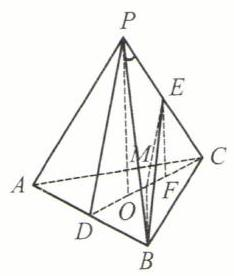
\includegraphics[width=0.2\textwidth]{bodyxb/src/bo_d20cdrf7aajc73bfmvhg_152_605_934_234_276_0.jpg}
\end{center}


[第 68(2)①②题]

\begin{center}
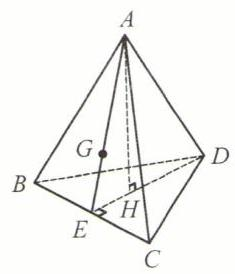
\includegraphics[width=0.2\textwidth]{bodyxb/src/bo_d20cdrf7aajc73bfmvhg_152_917_929_235_274_0.jpg}
\end{center}


[第 68(3)题]

(3) $\sqrt{7}a$ 提示:如图, $H$ 是底面 $\bigtriangleup  {BCD}$ 的重心, ${AB} = {AC}$ . 取 ${BC}$ 的中点 $E$ ,则可得 ${DE}\bot {BC}$ . 又 $\angle {AED} = {60}^{ \circ  }$ ,

$\therefore {EH} = {AH} \cdot  \cot {60}^{ \circ  } = 3\sqrt{3}a \times  \dfrac{\sqrt{3}}{3} = {3a},{AE} = {6a},G$ 为 $\bigtriangleup {ABC}$ 的重心, ${EG} = {2a}$ . 由余弦定理得 ${GH} =$  $\sqrt{{\left( 2a\right) }^{2} + {\left( 3a\right) }^{2} - 2 \cdot  {2a} \cdot  {3a} \cdot  \cos {60}^{ \circ  }} = \sqrt{7}a.$

69. (1) $\dfrac{\sqrt{3}}{3}$ 提示:如图,连接 ${AC}$ , ${BD}$ 交于点 $O$ ,由题 ${EO}//{PC}$ ,则 $\angle {BEO}$ 即异面直线 ${BE}$ , ${PC}$ 所成的角或其补角. 不妨设侧棱长与底面边长为 1,则 ${OE} = \dfrac{1}{2},{OB} = \dfrac{\sqrt{2}}{2},{BE} = \dfrac{\sqrt{3}}{2},\therefore \cos \angle {BEO} = \dfrac{{\left( \dfrac{\sqrt{3}}{2}\right) }^{2} + {\left( \dfrac{1}{2}\right) }^{2} - {\left( \dfrac{\sqrt{2}}{2}\right) }^{2}}{2 \cdot  \dfrac{1}{2} \cdot  \dfrac{\sqrt{3}}{2}} = \dfrac{\sqrt{3}}{3}$ ,即异面直线 ${BE}$ 与 ${PC}$ 所成角的余弦值为 $\dfrac{\sqrt{3}}{3}$ .

\begin{center}
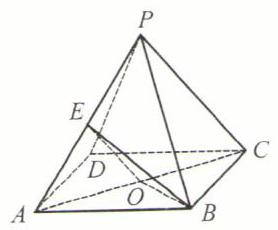
\includegraphics[width=0.2\textwidth]{bodyxb/src/bo_d20cdrf7aajc73bfmvhg_152_579_1754_278_230_0.jpg}
\end{center}


[第 69(1)题]

\begin{center}
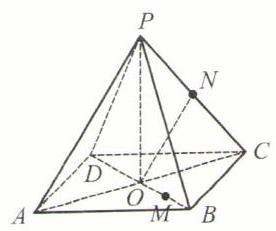
\includegraphics[width=0.2\textwidth]{bodyxb/src/bo_d20cdrf7aajc73bfmvhg_152_915_1745_276_231_0.jpg}
\end{center}


[第 69(2)题]

(2) $\dfrac{2\sqrt{5}}{5}$ 提示:如图, $M$ , $N$ 两点最短距离即异面直线 ${BD}$ , ${PC}$ 间的距离,连接 ${AC}$ , ${AC}$ 与 ${BD}$ 交于点 $O$ ,则 ${OC}$ 为 ${PC}$ 在底面的射影. ∵ ${BD} \bot  {AC},\therefore {BD} \bot  {PC},\therefore {BD} \bot$ 平面 ${PAC}$ ,过点 $O$ 作 ${ON} \bot  {PC}$ 于点 $N$ ,又 ${DB} \bot  {ON}$ ,

$\therefore {ON}$ 为 ${DB}$ 与 ${PC}$ 的公垂线. 在 Rt $\bigtriangleup {PON}$ 中, $\because \bigtriangleup {PON} \backsim  \bigtriangleup {PCO},\therefore \dfrac{ON}{CO} = \dfrac{PO}{PC}$ ,即 ${ON} = \dfrac{2\sqrt{5}}{5}$ ,即 $M,N$ 两点间最短距离为 $\dfrac{2\sqrt{5}}{5}$ .

70. 已知 $\bigtriangleup  {ABC}$ 为正三角形, ${PO} \bot$ 面 ${ABC},O$ 为 $\bigtriangleup  {ABC}$ 的中心.

取 ${BC}$ 中点 $D$ ,连接 ${MD}$ , ${PD}$ ,则 ${PD}\bot {BC}$ , ${AD}\bot {BC}$ , $\therefore {BC}\bot$ 面 ${PAD}$ , ${BC}\bot {MD}$ . 点 $D$ 到侧棱 ${PA}$ 的距离即 ${S}_{\bigtriangleup {MBC}}$ 最小时的高.

当 ${MD} \bot  {PA}$ 时, ${S}_{\bigtriangleup {PAD}} = \dfrac{1}{2}{PO} \cdot  {AD} = \dfrac{1}{2}{PA} \cdot  {MD}$ ,即 $8 \cdot  \sqrt{108} = \sqrt{112}{MD}$ ,得 ${MD} = \dfrac{{12}\sqrt{21}}{7}$ . $\therefore {S}_{\bigtriangleup {MBC}\min } = \dfrac{1}{2}{MD} \cdot  {BC} = \dfrac{{72}\sqrt{21}}{7}$ .

71. 如图, $\because {AB}$ 是圆的直径, $\therefore \angle {ACB} = {90}^{ \circ  }$ ,即 ${BC}\bot {AC}$ . $\because {PA}\bot$ 平面 ${ABC}$ , $\therefore {PA} \bot  {BC},\therefore {BC} \bot$ 平面 ${PAD},\therefore$ 直线 ${PB}$ 与平面 ${PAC}$ 所成角即 $\angle {BPC}$ . 不妨设 ${AB} = 6$ ,则 ${BC} = {AB} \times  \cos \angle {ABC} = 5$ ,又 $\because {PA} : {AB} = 4 : 3,\therefore {PA} = 8,{PB} = {10}$ . 在 $\bigtriangleup {PBC}$ 中, $\sin \angle {BPC} = \dfrac{BC}{PB} = \dfrac{1}{2},\therefore \angle {BPC} = {30}^{ \circ  }$ ,即直线 ${PB}$ 与平面 ${PAC}$ 所成角为 ${30}^{ \circ  }$ .

\begin{center}
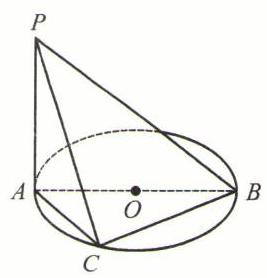
\includegraphics[width=0.2\textwidth]{bodyxb/src/bo_d20cdrf7aajc73bfmvhg_153_1186_557_267_278_0.jpg}
\end{center}


(第 71 题)

72. (1)证明: $\because {AB} \bot$ 平面 ${BCD},{CD}$ 在平面 ${BCD}$ 上, $\therefore {AB} \bot  {CD}$ . 又 ${BD} \bot  {CD}$ ,且 ${BD} \cap$  ${AB} = B,\therefore {CD} \bot$ 平面 ${ABD}$ . 又 $\because {CD}$ 在平面 ${ACD}$ 上, $\therefore$ 平面 ${ABD} \bot$ 平面 ${ACD}$ .

(2)过 $D$ 作 ${DE} \bot  {BC}$ 于点 $E$ , $\because {AB} \bot  {DE}$ , $\therefore {DE} \bot$ 平面 ${ABC}$ , $\therefore {DE} \bot  {AC}$ . 过点 $E$ 作 ${EF}\bot {AC}$ 于点 $F,\therefore {AC}\bot$ 平面 ${DEF}$ ,则 ${AC}\bot {DF}$ .

$\because \angle {DFE}$ 即二面角 $B - {AC} - D$ 的平面角,设 ${BD} = x$ ,则 ${AB} = {BC} = {2x}$ .

在 $\mathrm{{Rt}} \bigtriangleup  {BDC}$ 中, ${CD} = \sqrt{3}x,{BD} \cdot  {CD} = {BC} \cdot  {DE}$ ,则 ${DE} = \dfrac{\sqrt{3}}{2}x,{BE} = \dfrac{1}{2}x,{CE} = \dfrac{3}{2}x$ . 由 $\mathrm{{Rt}} \bigtriangleup  {CEF} \sim  \mathrm{{Rt}} \bigtriangleup  {CAB}$ ,

$\therefore \dfrac{EF}{CE} = \dfrac{AB}{AC},\;\therefore {EF} = \dfrac{3\sqrt{2}}{4}x$ . 则在 Rt $\bigtriangleup  {DEF}$ 中, $\sin \angle {DFE} = \dfrac{DE}{DF} = \dfrac{\dfrac{\sqrt{3}}{2}x}{\dfrac{\sqrt{30}}{4}x} = \dfrac{\sqrt{10}}{5}$ ,

$\therefore$ 二面角 $B - {AC} - D$ 的正弦值为 $\dfrac{\sqrt{10}}{5}$ .

73. (1) $\because {BC}\bot {AC}$ ,且 ${BC}\bot {PC},\therefore {BC}\bot$ 平面 ${ACP}.\therefore \bigtriangleup {ABP}$ 在平面 ${ACP}$ 上的射影即 $\bigtriangleup {ACP}$ .

又 ${PB} = \sqrt{13},{BC} = 3,\therefore {PC} = 2$ . 又 $\angle {PAC} = {30}^{ \circ  },\therefore {AC} = 2\sqrt{3},{AP} = 4$ .

在 $\mathrm{{Rt}} \bigtriangleup  {ACB}$ 中, ${AB} = \sqrt{A{C}^{2} + B{C}^{2}} = \sqrt{21}.\;\therefore$ 在 $\bigtriangleup  {APB}$ 中, ${AP} = 4,{BP} = \sqrt{13},{AB} = \sqrt{21}$ ,由海伦公式,

令 $p = \dfrac{{AP} + {BP} + {AB}}{2},{S}_{\bigtriangleup {APB}} = \sqrt{p\left( {p - 4}\right) \left( {p - \sqrt{13}}\right) \left( {p - \sqrt{21}}\right) } = 4\sqrt{3},\therefore \;\cos \theta  = \dfrac{{S}_{\bigtriangleup {APC}}}{{S}_{\bigtriangleup {APB}}}$  $= \dfrac{2\sqrt{3}}{4\sqrt{3}} = \dfrac{1}{2},\therefore \theta  = {60}^{ \circ  }$ ,即二面角 $B - {PA} - C$ 的度数为 ${60}^{ \circ  }$ .

\begin{center}
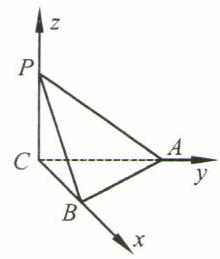
\includegraphics[width=0.2\textwidth]{bodyxb/src/bo_d20cdrf7aajc73bfmvhg_153_1225_1424_220_259_0.jpg}
\end{center}


[第 73(2)题]

(2)如图,建立空间直角坐标系,则 $C\left( {0,0,0}\right) ,B\left( {3,0,0}\right) ,A\left( {0,2\sqrt{3},0}\right) ,P\left( {0,0,2}\right)$ ,则 $\vv{PA} = (0,2$  $\sqrt{3}, - 2),\vv{PB} = \left( {3,0, - 2}\right)$ . 设 $O\left( {x,y,z}\right)$ ,则 $\vv{CO} = \left( {x,y,z}\right) ,\;\because \;\vv{CO}\bot \vv{PA}$ 且 $\vv{CO}\bot \vv{PB}$ ,则 $\left\{  \begin{array}{l} 2\sqrt{3}y - {2z} = 0, \\  {3x} - {2z} = 0, \end{array}\right.$ 则 $O\left( {{2t},\sqrt{3}t,{3t}}\right)$ . 又 ${PAB}$ 平面: ${2x} + \sqrt{3}y + {3z} = 6$ 且 $O$ 在平面 ${PAB}$ 上, $\therefore$  ${4t} + {3t} + {9t} = 6,\;\therefore \;t = \dfrac{3}{8},\;\therefore \;O\left( {\dfrac{3}{4},\dfrac{3\sqrt{3}}{8},\dfrac{9}{8}}\right)$ . 故点 $O$ 到平面 ${PAC}$ 的距离为 $\dfrac{3}{4}$ .

74. (1) 如图,取 ${AB},{AC}$ 的中点,分别记为 $D,E$ . 取 ${BD},{EC}$ 的中点,分别记为 $N,F$ . 连接 ${PD}$ ,

\begin{center}
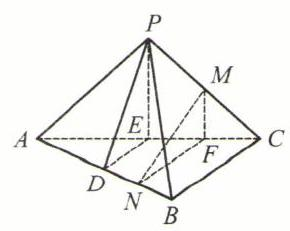
\includegraphics[width=0.2\textwidth]{bodyxb/src/bo_d20cdrf7aajc73bfmvhg_153_1156_1825_290_231_0.jpg}
\end{center}


(第 74 题)

${PE},{DE},{MF},{NF}$ .

$\because {PA} = {PB},\therefore {PD} \bot  {AB}$ . 又 $D,E$ 为 ${AB},{AC}$ 中点, $\therefore {DE}//{BC}$ .

又 ${BC} \bot$ 平面 ${PAB},\therefore {DE} \bot  {AB}$ ,而 ${PD} \cap  {DE} = D$ ,

$\therefore {AB} \bot$ 平面 ${PDE}$ . 而 ${NF}//{DE},{MF}//{PE}$ ,

$\therefore$ 平面 ${PDE}//$ 平面 ${MNF},\therefore {AB} \bot$ 平面 ${MNF}$ ,且 ${MN} \subset$ 平面 ${MNF}$ ,

$\therefore {MN}\bot {AB}$ .

(2)如图, $\because \angle {APB} = {90}^{ \circ  }$ 且 ${AP} = {BP},{AB} = 4$ ,

$\therefore {AP} = {BP} = 2\sqrt{2}$ . 又 ${CB} \bot$ 平面 ${PAB}$ ,

$\therefore {CB} \bot  {PB}$ . $\therefore$ 在 Rt $\bigtriangleup  {PBC}$ 中, ${PB} = 2\sqrt{2},{BC} = 2,M$ 为 ${PC}$ 的中点, $\therefore {BM} = \dfrac{PC}{2} = \sqrt{3}$ .

$\therefore$ 在 Rt $\bigtriangleup  {MNB}$ 中, ${NB} = 1,{MB} = \sqrt{3},\therefore {MN} = \sqrt{3 - 1} = \sqrt{2}$ .

75. 设正三棱锥 $P - {ABC}$ 的底面边长为 ${2a}$ ,侧棱长为 $b,{PH} = x,{DH} = {3x}$ .

$\because$ 正三棱锥 $P - {ABC}$ 中, $A$ 在侧面 ${PBC}$ 上的射影为 $H$ ,

$\therefore \angle {ADP}$ 即侧面与底面所成二面角, $\therefore \cos \angle {ADP} = \dfrac{DH}{AD} = \dfrac{\sqrt{3}x}{a}$ .

$\because A{H}^{2} = {b}^{2} - {x}^{2} = 3{a}^{2} - 9{x}^{2},{4x} = \sqrt{{b}^{2} - {a}^{2}},\;\therefore a = 2\sqrt{3}x,\;\therefore \cos \angle {ADP} = \dfrac{1}{2},\;\therefore \angle {ADP} = \dfrac{\pi }{3}$ . 即侧面与底面所成二面角为 $\dfrac{\pi }{3}$ .

76. (1)①过点 $P$ 作 ${PO}\bot$ 平面 ${ABC}$ 于点 $O$ ,过点 $P$ 作 ${PD}\bot {AB}$ 于点 $D$ . 由已知, $O$ 落在 ${CD}$ 上. $\because {PA},{PB},{PC}$ 两两垂直, $\therefore {PC} \bot$ 平面 ${ABP},\therefore {PC} \bot  {PD}$ .

\begin{center}
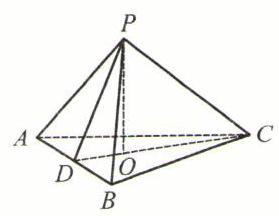
\includegraphics[width=0.2\textwidth]{bodyxb/src/bo_d20cdrf7aajc73bfmvhg_154_1239_582_279_216_0.jpg}
\end{center}


(第 76 题)

$\because {PA} \bot  {PB},{PA} = {PB} = 1,\;\therefore \;{AD} = {PD} = \dfrac{\sqrt{2}}{2}$ .

又 $\because {PC} \bot  {PA},{PC} = 2$ ,

$\therefore {AC} = \sqrt{5},{CD} = \sqrt{{\left( \dfrac{\sqrt{2}}{2}\right) }^{2} + {2}^{2}} = \dfrac{3\sqrt{2}}{2}$ ,则 ${PO} = \dfrac{{PD} \cdot  {PC}}{CD} = \dfrac{2}{3}$ ,即点 $P$ 到底面 ${ABC}$ 的距离为 $\dfrac{2}{3}$ .

② $\because {PO} = \dfrac{2}{3},\therefore {OC} = \sqrt{{2}^{2} - {\left( \dfrac{2}{3}\right) }^{2}} = \dfrac{4\sqrt{2}}{3}$ ,则 ${S}_{\bigtriangleup {OBC}} = \dfrac{1}{2}{OC} \cdot  {BD} = \dfrac{1}{2} \cdot  \dfrac{4\sqrt{2}}{3} \cdot  \dfrac{\sqrt{2}}{2} = \dfrac{2}{3}$ .

又 ${S}_{\bigtriangleup {PBC}} = \dfrac{1}{2} \cdot  1 \cdot  2 = 1,\therefore \cos \theta  = \dfrac{{S}_{\bigtriangleup {OBC}}}{{S}_{\bigtriangleup {PBC}}} = \dfrac{2}{3}$ ,则 $\sin \theta  = \sqrt{1 - {\cos }^{2}\theta } = \dfrac{\sqrt{5}}{3}$ ,即二面角 $P - {BC} - A$ 的正弦值为 $\dfrac{\sqrt{5}}{3}$ .

(2)三条侧棱在底面的投影相等,即 $\bigtriangleup  {ABC}$ 外接圆的半径. 由 $\dfrac{b}{\sin B} = {2R}$ ,得 $R = \dfrac{b}{2\sin B} = 3$ ,

$\therefore H = R \cdot  \tan {75}^{ \circ  } = 3\left( {2 + \sqrt{3}}\right)$ .

(3) $\because c$ , $a$ 是方程 $3{x}^{2} - {27x} + {32} = 0$ 两根, $\therefore \left\{  {\begin{array}{l} a + c = 9, \\  {ac} = \dfrac{32}{3}, \end{array}\therefore {b}^{2} = {a}^{2} + {c}^{2} - {2ac} \cdot  \cos B = {\left( a + c\right) }^{2} - {3ac} = {49}}\right.$ ,即 $b = 7$ . 设三角形 ${ABC}$ 内切圆的半径为 $r$ ,则 $S = \dfrac{1}{2}\left( {a + b + c}\right) r = \dfrac{1}{2} \times  {16} \times  r = \dfrac{8\sqrt{3}}{3}$ , $\therefore r = \dfrac{\sqrt{3}}{3}$ . 又侧面与底面成 ${45}^{ \circ  }$ 角, $\therefore h = r = \dfrac{\sqrt{3}}{3}$ . 77. 由题意可知截面为矩形,设长 (平行于 ${PN}$ 的边的长) 为 $x$ ,宽 (平行于 ${AB}$ 的边的长) 为 $y$ ,则 $x + \dfrac{y}{2} = 1$ , $\therefore {xy} = 2 \cdot  x \cdot  \dfrac{y}{2} \leq  2 \cdot  {\left( \dfrac{x + y}{2}\right) }^{2} = \dfrac{1}{2}$ . 当且仅当 $x = \dfrac{y}{2}$ 时,即 $x = \dfrac{1}{2},y = 1$ 时等号成立. 即当 $Q$ 为 ${BP}$ 的中点时,截面面积最大,为 $\dfrac{1}{2}$ .

78. (1) $\because {A}_{1}D \bot  {A}_{1}B,{A}_{2}C \bot  {A}_{2}B,\therefore$ 三棱锥中 ${AB} \bot  {AD},{AB} \bot  {AC},\therefore {AB} \bot$ 平面 ${ACD}$ .

又 ${CD}$ 在平面 ${ACD}$ 上, $\therefore {AB} \bot  {CD}$ .

(2) $B,C$ 是 ${A}_{1}{A}_{2},{A}_{2}{A}_{3}$ 的中点, $\therefore {A}_{1}D = {A}_{3}D = {10},{A}_{1}B = {A}_{2}B = 4$ . 过点 $D$ 作 ${DE}\bot {A}_{2}{A}_{3}$ 于点 $E$ ,则 ${DE} = 8$ .

在 $\mathrm{{Rt}} \bigtriangleup  {DEA}_{3}$ 中, $E{A}_{3} = 6,\;\therefore \;{A}_{2}{A}_{3} = {16}$ ,

$\therefore {A}_{2}C = C{A}_{3} = 8,{CE} = 2,\therefore {S}_{\bigtriangleup {BCD}} = {36},{S}_{\bigtriangleup {CDA}} = {32}$ .

$\because {AB} \bot$ 平面 ${ACD}$ ,

$\therefore \cos \theta  = \dfrac{{S}_{\bigtriangleup {ACD}}}{{S}_{\bigtriangleup {BCD}}} = \dfrac{32}{36} = \dfrac{8}{9}$ ,则 $\tan \theta  = \dfrac{\sqrt{17}}{8}$ ,即侧面 ${ACD}$ 和底面 ${BCD}$ 所成二面角的正切值为 $\dfrac{\sqrt{17}}{8}$ .

79. $\because \angle {DAB} = \angle {ABC} = {90}^{ \circ  },\therefore {BC}//{AD}$ 且 ${AC} = \sqrt{2}$ ,且 $\angle {BAD} = {45}^{ \circ  }$ .

$\because {CD} = \sqrt{2},\because {AC} = {CD} = \sqrt{2}$ 且 ${AD} = 2,\therefore \angle {ACD} = {90}^{ \circ  }.\therefore {DC}\bot {AC}$ .

$\because {PA} \bot$ 平面 ${ABCD}.\therefore {PA} \bot  {CD}$ ,又 ${AC} \cap  {PA} = A,\therefore {CD} \bot$ 平面 ${PAC}$ .

80. 如图,在三棱锥 $P - {ABC}$ 中, ${PO} \bot$ 平面 ${ABC}$ , $O$ 为 $\bigtriangleup  {ABC}$ 的垂心. 求证: $A$ 在平面 ${PBC}$ 内的射影是 $\bigtriangleup {PBC}$ 的垂心.

\begin{center}
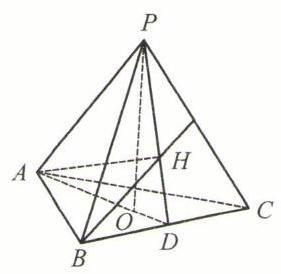
\includegraphics[width=0.2\textwidth]{bodyxb/src/bo_d20cdrf7aajc73bfmvhg_155_1175_127_281_274_0.jpg}
\end{center}


(第 80 题)

证明: 连接 ${AO}$ 交 ${BC}$ 于点 $D,\because {PO} \bot$ 平面 ${ABC},{BC}$ 在平面 ${ABC}$ 上, $\therefore {PO} \bot  {BC}$ .

$\because O$ 为 $\bigtriangleup  {ABC}$ 垂心, $\therefore {BC}\bot {AO}.\;\because {PO} \cap  {AO} = O,\therefore {BC}\bot$ 平面 ${PAD}$ ,

$\therefore {BC}\bot {PA}$ .

同理 ${AB} \bot  {PC}.\because {BC}$ 在平面 ${PBC}$ 上, $\therefore$ 平面 ${PBC} \bot$ 平面 ${PAD}$ . 作 ${AH} \bot  {PD}$ 于点 $H$ ,则 ${AH} \bot$ 平面 ${PBC}$ ,

$\therefore {BH}$ 是 ${AB}$ 在平面 ${PBC}$ 内的射影. $\because {AB} \bot  {PC}$ ,由三垂线定理得 ${BH} \bot  {PC}$ . 又 ${BC} \bot$  ${PD},\therefore H$ 是 $\bigtriangleup {PBC}$ 的垂心,得证.

81. 如图,正三棱锥 $P - {ABC}$ 中, ${AB} = {BC} = {CA} = 2$ ,高 ${PO} = \dfrac{\sqrt{6}}{6}$ . ${AB}$ 的中点为 $M$ ,则 $O$ 在 ${MC}$ 上且 ${MO} = \dfrac{\sqrt{3}}{3},{PM} = \dfrac{\sqrt{2}}{2}$ .

\begin{center}
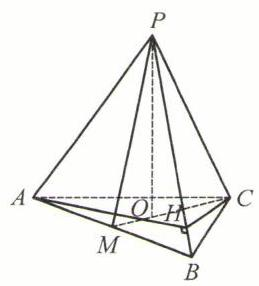
\includegraphics[width=0.2\textwidth]{bodyxb/src/bo_d20cdrf7aajc73bfmvhg_155_1194_487_259_286_0.jpg}
\end{center}


(第 81 题)

在 $\bigtriangleup {PMB}$ 中, ${PB} = \sqrt{P{M}^{2} + M{B}^{2}} = \dfrac{\sqrt{6}}{2}$ .

过点 $A$ 作 ${AH}\bot {PB}$ ,连接 ${CH}.\because \bigtriangleup {PAB} \cong  \bigtriangleup {PCB},\therefore {CH}\bot {PB}$ .

在 $\bigtriangleup {PAB}$ 中, ${AH} = \dfrac{{AB} \cdot  {PM}}{PB} = \dfrac{2 \times  \dfrac{\sqrt{2}}{2}}{\dfrac{\sqrt{6}}{2}} = \dfrac{2\sqrt{3}}{3}$ ,则在 $\bigtriangleup {AHC}$ 中,

$\cos \angle {AHC} = \dfrac{A{H}^{2} + C{H}^{2} - A{C}^{2}}{2 \cdot  {AH} \cdot  {CH}} =  - \dfrac{1}{2}$ ,又 $\angle {AHC}$ 即二面角的平面角, $\therefore$ 两侧面所成二面角为 ${120}^{ \circ  }$ . 82. 如图, ${SE}\bot {BC},{BF}\bot {SC}$ ,其中 $E$ , $F$ 都是垂足. (1) $\cot \alpha  = \dfrac{AO}{SO},\tan \beta  = \dfrac{SO}{OE},\therefore \cot \alpha  \cdot  \tan \beta  = \dfrac{AO}{OE} = \sqrt{2}$ . (2) $\sin \alpha  = \dfrac{OF}{OC},\tan \dfrac{\gamma }{2} = \dfrac{OB}{OF},\therefore \sin \alpha  \cdot  \tan \dfrac{\gamma }{2} = \dfrac{OB}{OC} = 1$ . (3) 由(2) $\tan \dfrac{\gamma }{2} = \dfrac{1}{\sin \alpha },\;\therefore \;\cos \gamma  = \dfrac{{\cos }^{2}\alpha }{{\cos }^{2}\alpha  - 2}$ . 由 $\left( 1\right) \tan \beta  = \sqrt{2}\tan \alpha ,\;\therefore \;{\cos }^{2}\beta  = \dfrac{{\cos }^{2}\alpha }{2 - {\cos }^{2}\alpha }$ ,即 $\cos \gamma  + {\cos }^{2}\beta  = 0$ . 83. (1) $\because {PA} \bot$ 平面 ${ABCD}$ , $\therefore {PA} \bot  {DC}$ . 又 $\because {DC} \bot  {PD}$ , $\therefore {DC} \bot$ 平面 ${PAD}$ , $\therefore {DC}\bot {AD}$ .

\begin{center}
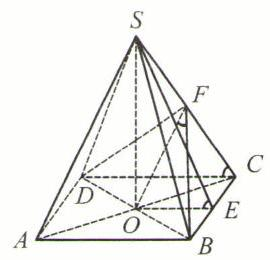
\includegraphics[width=0.2\textwidth]{bodyxb/src/bo_d20cdrf7aajc73bfmvhg_155_1183_960_270_260_0.jpg}
\end{center}


(第 82 题)

又 $\because {ABCD}$ 为菱形, $\therefore {ABCD}$ 为正方形, $\therefore {AB} \bot  {BC}$ .

又 $\because {PA} \bot  {BC},\therefore {BC} \bot$ 平面 ${PAB},\therefore {BC} \bot  {PB}$ .

又 $\because {PB} \bot$ 平面 ${EFAD},\therefore {PB} \bot  {EF},\therefore {EF}//{BC},\therefore {EF} \bot$ 平面 ${PAB}$ .

(2) ${S}_{ADEF} = \dfrac{1}{2}\left( {{AD} + {EF}}\right)  \cdot  {AF} = \dfrac{816}{125}$ .

(3) $\angle {FAB}$ 是二面角 $F - {AD} - B$ 的平面角, $\therefore \cos \angle {FAB} = \dfrac{AF}{AB} = \dfrac{3}{5}$ .

\begin{center}
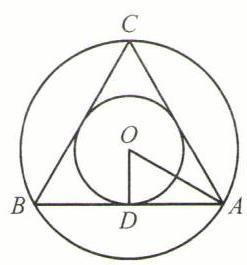
\includegraphics[width=0.2\textwidth]{bodyxb/src/bo_d20cdrf7aajc73bfmvhg_155_1203_1551_247_265_0.jpg}
\end{center}


(第 85 题)

84. $C$ 提示: ${S}_{\text{ 侧 }} = {\pi dh} = {\pi S},\;\therefore$ 选 $C$ .

85. B 提示:如图, ${OD}$ 为内圆柱底面半径,在 $\mathrm{{Rt}} \bigtriangleup  {OAD}$ 中, $\angle {OAD} = {30}^{ \circ  }$ ,

$\therefore {AO} = {2OD}$ ,

$\therefore \dfrac{{S}_{\text{ 侧内 }}}{{S}_{\text{ 侧外 }}} = \dfrac{\pi {d}_{\text{ 内 }}h}{\pi {d}_{\text{ 外 }}h} = \dfrac{OD}{AO} = \dfrac{1}{2},\;\therefore \;$ 选 B.

86. C 提示: ${2\pi r} = 8 \cdot  \cos {30}^{ \circ  },{S}_{\text{ 侧 }} = {2\pi rh} = 8 \cdot  \cos {30}^{ \circ  } \cdot  \left( {8 \cdot  \sin {30}^{ \circ  }}\right)  = {16}\sqrt{3}{\mathrm{\;{cm}}}^{2}$ ,

$\therefore$ 选 C.

87. A 提示: 设所求截面底边长为 $x$ ,则 ${\left( \dfrac{x}{2}\right) }^{2} = {20}^{2} - {12}^{2} \Rightarrow  x = {32},\therefore {S}_{\text{ 极 }} = {32} \times  {15} = {480}{\mathrm{\;{cm}}}^{2},\therefore$ 选 A.

88. $C$ 提示:设原圆柱高 $h$ ,底面直径 $d$ . 则 ${S}_{\text{ 原侧 }} = {\pi dh},{S}_{\text{ 新侧 }} = \pi  \cdot  {4d} \cdot  {3h} = {12\pi dh}.\therefore \dfrac{{S}_{\text{ 新侧 }}}{{S}_{\text{ 原侧 }}} = {12},\therefore$ 选 C.

89. (1) ${\pi S}$ 提示: 设圆柱高 $h$ ,底面直径 $d$ ,则 $S = {dh}$ ,则 ${S}_{\text{ 侧 }} = {\pi dh} = {\pi S}$ .

(2) $\dfrac{3}{2}{\pi Q}$ 提示:由题 $d = h = \sqrt{Q}$ . 则 ${S}_{\text{ 表 }} = {\pi dh} + \dfrac{\pi {d}^{2}}{4} \cdot  2 = {\pi Q} + \dfrac{\pi Q}{2} = \dfrac{3}{2}{\pi Q}$ .

3 ${16}\sqrt{3} + \dfrac{24}{\pi }{\mathrm{{cm}}}^{2}$ 或 ${16}\sqrt{3} + \dfrac{8}{\pi }$ 提示:① ${\pi d} = 4\sqrt{3}\mathrm{\;{cm}},h = 4\mathrm{\;{cm}}$ ,则 ${S}_{\text{ 全 }} = {\pi dh} + \dfrac{\pi {d}^{2}}{4} \cdot  2 = {16}\sqrt{3} + \dfrac{24}{\pi }{\mathrm{{cm}}}^{2}$

② ${\pi d} = 4\mathrm{\;{cm}},h = 4\sqrt{3}\mathrm{\;{cm}}$ ,则 ${S}_{\text{ 全 }} = {\pi dh} + \dfrac{\pi {d}^{2}}{4} \cdot  2 = {16}\sqrt{3} + \dfrac{8}{\pi }{\mathrm{\;{cm}}}^{2}$ .

90. (1) ${2\pi }$ 提示: 设这个正方形的边长为 $a,{S}_{\text{ 全 }} = {2\pi a} \cdot  a + {2\pi }{a}^{2} = {4\pi }{a}^{2},{S}_{\text{ 轴 }} = {2a} \cdot  a = 2{a}^{2},\therefore \dfrac{{S}_{\text{ 全 }}}{{S}_{\text{ 轴 }}} = {2\pi }$ .

(2) ${16}{\pi }^{2}$ 提示:由 ${S}_{\text{ 底 }} = {4\pi }$ ,可得 $r = 2,{S}_{\text{ 侧 }} = {\left( 2\pi r\right) }^{2} = {16}{\pi }^{2}$ .

91. (1) 2 提示: ${A}_{1}{B}_{1} = 2\sqrt{{13}^{2} - {5}^{2}} = {24}$ ,又 ${S}_{{A}_{1}{B}_{1}{BA}} = {48},\therefore {A}_{1}A = \dfrac{48}{24} = 2$ .

(2) $\dfrac{\sqrt{2}}{2}$ 提示: $\angle {A}_{1}{O}_{1}{B}_{1} = \dfrac{2\pi }{4} = \dfrac{\pi }{2},\therefore {O}_{1}O$ 与截面的距离是 ${O}_{1}{A}_{1}$ 的 $\dfrac{\sqrt{2}}{2}$ 倍.

(3) $\dfrac{2R}{h}\sin \dfrac{\theta }{2}a$ 或 $\dfrac{2R}{h}\cos \dfrac{\theta }{2}$ 提示: ${O}_{1}O//{A}_{1}A$ . 则 $\angle B{A}_{1}A$ 即 ${O}_{1}O$ 与 ${A}_{1}B$ 所成角或其补角. 又 ${O}_{1}{A}_{1}$ 和 ${OB}$ 成 $\theta$ 角,有

两种可能,① $\angle {AOB} = \theta ,{AO} = {BO} = R,\therefore {AB} = {2R}\sin \dfrac{\theta }{2}$ ,在 $\mathrm{{Rt}} \bigtriangleup  {A}_{1}{AB}$ 中, ${A}_{1}A = h$ .

$\therefore \tan \angle B{A}_{1}A = \dfrac{AB}{A{A}_{1}} = \dfrac{{2R}\sin \dfrac{\theta }{2}}{h}$ . 即 ${O}_{1}O$ 与 ${A}_{1}B$ 所成角的正切值为 $\dfrac{2R}{h} \cdot  \sin \dfrac{\theta }{2}$ .

② $\angle {AOB} = \pi  - \theta ,{AO} = {BO} = R\;\therefore \;{AB} = {2R}\cos \dfrac{\theta }{2}\;\therefore \;\tan \angle B{A}_{1}A = \dfrac{2R}{h} \cdot  \cos \dfrac{\theta }{2}$ .

92. 如图, $\angle B{O}^{\prime }{A}^{\prime } = {90}^{ \circ  },{A}^{\prime }{O}^{\prime } = B{O}^{\prime } = 6\mathrm{\;{cm}}$ . 则 ${A}^{\prime }B = 6\sqrt{2}\mathrm{\;{cm}}$ ,

\begin{center}
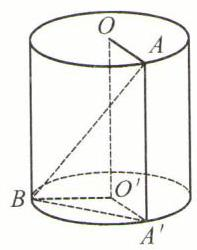
\includegraphics[width=0.2\textwidth]{bodyxb/src/bo_d20cdrf7aajc73bfmvhg_156_1329_838_197_250_0.jpg}
\end{center}


(第 92 题)

在 $\mathrm{{Rt}}\bigtriangleup A{A}^{\prime }B$ 中, ${A}^{\prime }B = 6\sqrt{2}\mathrm{\;{cm}},A{A}^{\prime } = {12}\mathrm{\;{cm}},\;\therefore \;{AB} = \sqrt{{\left( 6\sqrt{2}\right) }^{2} + {12}^{2}} = 6\sqrt{6}\mathrm{\;{cm}}$ .

93. 弦长 $l = 2 \cdot  2 \cdot  \tan \dfrac{{120}^{ \circ  }}{2} = 4\sqrt{3}\mathrm{\;{cm}}$ . 则 $S = 4\sqrt{3} \cdot  {10} = {40}\sqrt{3}{\mathrm{\;{cm}}}^{2}$ .

94. B 提示: 设对角线长为 $a$ ,轴截面对角线与底面所成角为 $\theta$ .

则 $S = \pi  \cdot  \left( {a\cos \theta }\right)  \cdot  \left( {a\sin \theta }\right)  = \pi {a}^{2} \cdot  \sin \theta  \cdot  \cos \theta  = \dfrac{\pi {a}^{2}}{2}\sin {2\theta }$

$\therefore$ 当 ${2\theta } = \dfrac{\pi }{2}$ 即 $\theta  = \dfrac{\pi }{4}$ 时, ${S}_{\max } = \dfrac{\pi {a}^{2}}{2},\;\therefore$ 选 B.

95. B 提示: $S = {2\pi r} \cdot  l = {4\pi },\therefore l = \dfrac{2}{r}$ ,则轴截面对角线长 $\sqrt{{l}^{2} + {\left( 2r\right) }^{2}} = \sqrt{\dfrac{4}{{r}^{2}} + 4{r}^{2}} \geq  \sqrt{2 \cdot  \sqrt{4 \cdot  4}} = 2\sqrt{2}$ ,

$\therefore$ 当且仅当 $\dfrac{4}{{r}^{2}} = 4{r}^{2}$ ,即 $r = 1$ 时,取等号. 此时 $l = \dfrac{2}{r} = 2,\therefore l = {2r},\therefore$ 选 B.

\begin{center}
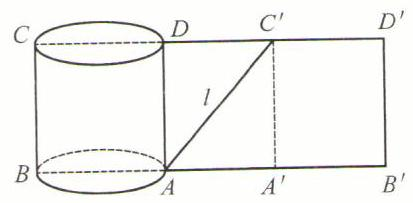
\includegraphics[width=0.3\textwidth]{bodyxb/src/bo_d20cdrf7aajc73bfmvhg_156_1121_1340_413_203_0.jpg}
\end{center}


(第 96 题)

96. D 提示: 如图, $l = \sqrt{{\left( \dfrac{5\pi }{2}\right) }^{2} + {5}^{2}} = \dfrac{5}{2}\sqrt{{\pi }^{2} + 4}\mathrm{\;{cm}}$ ,

$\therefore$ 选 D.

97. 设 $A{A}_{1}$ 是圆柱的一条母线.

(1)如图,作 ${O}_{1}H\bot {A}_{1}B$ 于点 $H$ ,又 $\because A{A}_{1}\bot {O}_{1}H$ ,

$\therefore {O}_{1}H \bot$ 平面 $A{A}_{1}B$ ,且 $O{O}_{1}//$ 平面 $A{A}_{1}B$ ,

又 $O{O}_{1} \bot  {O}_{1}H$ 且 ${O}_{1}H = \dfrac{3\sqrt{3}}{2},\therefore {AB}$ 和 $O{O}_{1}$ 距离为 $\dfrac{3\sqrt{3}}{2}$ .

(2)如图,设轴截面边长为 ${2a}$ ,则底面半径为 $a$ ,高为 ${2a}$ . 在 $\mathrm{{Rt}} \bigtriangleup  {AA}_{1}B$ 中, $\angle {ABA}_{1} = a$ , ${AA}_{1} = {2a}$ ,

$\therefore {A}_{1}B = \dfrac{2a}{\tan \alpha }$ . 又 ${O}_{1}{A}_{1} = {O}_{1}B = a,\;\therefore {O}_{1}H = \sqrt{{a}^{2} - \dfrac{{a}^{2}}{{\tan }^{2}\alpha }} = a \cdot  \sqrt{1 - {\cot }^{2}\alpha }$ .

(3)如图,将柱面上 ${AB}$ 的图展开成平面. 柱面上 ${AB}$ 的最短距离即 $\sqrt{{\left( \alpha R\right) }^{2} + {h}^{2}} = \sqrt{{\alpha }^{2}{R}^{2} + {h}^{2}}$ 或 $\sqrt{{\left( \pi  - x\right) }^{2}{R}^{2} + {h}^{2}}$ .

\begin{center}
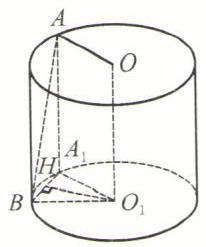
\includegraphics[width=0.2\textwidth]{bodyxb/src/bo_d20cdrf7aajc73bfmvhg_156_328_1858_206_247_0.jpg}
\end{center}


[第 97(1)题]

\begin{center}
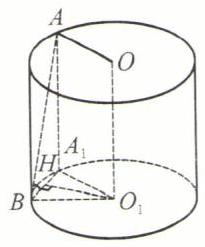
\includegraphics[width=0.2\textwidth]{bodyxb/src/bo_d20cdrf7aajc73bfmvhg_156_618_1855_205_247_0.jpg}
\end{center}


[第 97(2)题]

\begin{center}
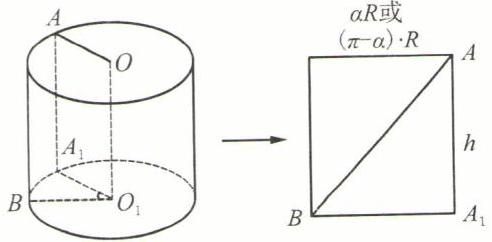
\includegraphics[width=0.4\textwidth]{bodyxb/src/bo_d20cdrf7aajc73bfmvhg_156_910_1849_492_242_0.jpg}
\end{center}


[第 97(3)题]

98. (1) $\because A{A}_{1} \bot  {BC},{AC} \bot  {BC},\therefore {BC} \bot$ 平面 $A{A}_{1}C,\therefore$ 面 $A{A}_{1}C \bot$ 面 ${A}_{1}{BC}$ .

( 2 )作 ${AF}\bot {A}_{1}C$ 于点 $F$ , ${FE}\bot {A}_{1}B$ 于点 $E$ ,则 $\angle {AEF}$ 是二面角 $A - {A}_{1}B - C$ 的平面角,

$\therefore \angle {AEF} = \alpha .\;\because \;\cos \beta  = \dfrac{AC}{AB},\cos \gamma  = \dfrac{{A}_{1}C}{{A}_{1}B},\sin \alpha  = \dfrac{AF}{AE},\;\therefore \;\dfrac{\cos \beta }{\cos \gamma } = \dfrac{AC}{AB} \cdot  \dfrac{{A}_{1}B}{{A}_{1}C} = \dfrac{{AF} \cdot  {A}_{1}C}{A{A}_{1}} \cdot  \dfrac{{A}_{1}A}{{AE} \cdot  {A}_{1}B}$ . $\dfrac{{A}_{1}B}{{A}_{1}C} = \dfrac{AF}{AE} = \sin \alpha$ . 即 $\sin \alpha  = \dfrac{\cos \beta }{\cos \gamma }$ 得证.

99. 如图,设圆柱中,点 $P$ 和 $Q$ 所在的平行于圆柱底面的截面圆心分别为 ${O}_{1}$ 和 ${O}_{2},P$ 在面 ${O}_{2}$ 上的射影为 ${P}_{1}\because$ 边长 15 $\mathrm{{cm}},\therefore$ 圆柱底面半径 $r = \dfrac{15}{2\pi }\mathrm{{cm}}$ . 又劣弧 ${P}_{1}Q$ 的长为 $5\mathrm{\;{cm}},\therefore \angle {P}_{1}{O}_{2}Q = \dfrac{2\pi }{3}$ ,

$\therefore {P}_{1}Q = 2 \cdot  r \cdot  \sin \dfrac{\angle {P}_{1}{O}_{2}Q}{2} = 2 \cdot  \dfrac{15}{2\pi } \cdot  \sin \dfrac{\pi }{3} = \dfrac{{15}\sqrt{3}}{2\pi }\mathrm{{cm}}$ . 在 Rt $\bigtriangleup  P{P}_{1}Q$ 中, $P{P}_{1} = 8\mathrm{\;{cm}},{P}_{1}Q = \dfrac{{15}\sqrt{3}}{2\pi }\mathrm{{cm}}$ ,

$\therefore {PQ} = \sqrt{P{P}_{1}^{2} + {P}_{1}{Q}^{2}} = \sqrt{{64} + \dfrac{675}{4{\pi }^{2}}} = \dfrac{1}{2\pi } \cdot  \sqrt{{256}{\pi }^{2} + {675}}\mathrm{\;{cm}}$ .

\begin{center}
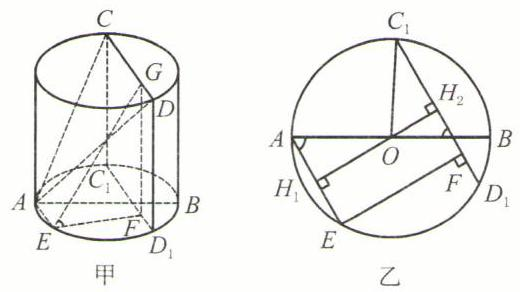
\includegraphics[width=0.4\textwidth]{bodyxb/src/bo_d20cdrf7aajc73bfmvhg_157_674_620_520_292_0.jpg}
\end{center}


(第 100 题)

\begin{center}
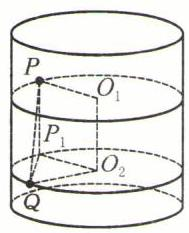
\includegraphics[width=0.2\textwidth]{bodyxb/src/bo_d20cdrf7aajc73bfmvhg_157_350_677_189_233_0.jpg}
\end{center}


(第 99 题)

100. 如图甲,过 $A$ 作 ${AE}//{C}_{1}{D}_{1}$ 交圆于 $E$ ,过 $E$ 作 ${EF}\bot {C}_{1}{D}_{1}$ 于点 $F$ ,作 ${FG}\bot {CD}$ 于点 $G$ . 连接 ${EG}$ ,则 $\angle {GEF} = {45}^{ \circ  }$ ,

$\therefore$ 在 $\mathrm{{Rt}} \bigtriangleup  {GFE}$ 中, ${GF} = {EF}$ . 如图乙为下底面截图,过圆心 $O$ 作 ${H}_{1}{H}_{2}//{EF}$ 交 ${AE}$ 于 ${H}_{1}$ ,交 ${C}_{1}{D}_{1}$ 于 ${H}_{2}$ ,则 $O{H}_{1} =$  $R \cdot  \sin {60}^{ \circ  } = \dfrac{\sqrt{3}}{2}R$ ,则 $O{H}_{2} = \sqrt{{R}^{2} - {\left( \dfrac{a}{2}\right) }^{2}} = \sqrt{{R}^{2} - \dfrac{{a}^{2}}{4}},\;\therefore \;h = {GF} = {EF} = O{H}_{1} + O{H}_{2} = \dfrac{\sqrt{3}}{2}R + \sqrt{{R}^{2} - \dfrac{{a}^{2}}{4}}$ 或 $\left| {O{H}_{1} - O{H}_{2}}\right|  = \left| {\dfrac{\sqrt{3}}{2}R - \sqrt{{R}^{2} - \dfrac{{a}^{2}}{4}}}\right| .$

101. A 提示: ${S}_{\text{ 侧 }} = {\pi rl} = {2\pi }{r}^{2},{S}_{\text{ 全 }} = {S}_{\text{ 侧 }} + {S}_{\text{ 底 }} = {2\pi }{r}^{2} + \pi {r}^{2} = {3\pi }{r}^{2},\;\therefore \dfrac{{S}_{\text{ 侧 }}}{{S}_{\text{ 全 }}} = \dfrac{{2\pi }{r}^{2}}{{3\pi }{r}^{2}} = \dfrac{2}{3},\;\therefore$ 选 A.

102. $C$ 提示: $\dfrac{{S}_{\text{ 单 }}}{{S}_{\text{ 全 }}} = \dfrac{\pi rl}{{\pi rl} + \pi {r}^{2}} = \dfrac{2}{3}$ ,得 $l = {2r},\sin \dfrac{\alpha }{2} = \dfrac{r}{l} = \dfrac{1}{2}$ ,即 $\sin \dfrac{\alpha }{2} = \dfrac{1}{2},\dfrac{\alpha }{2} = \dfrac{\pi }{6}$ ,得 $\alpha  = \dfrac{\pi }{3}$ , $\therefore$ 选 C.

103. A 提示: $\dfrac{1}{2}a{R}^{2} = {S}_{1}$ ,得 $R = \sqrt{\dfrac{2{S}_{1}}{a}} = \sqrt{\dfrac{8{S}_{1}}{3\pi }}$ . 扇形的弧长 $l = {aR} = \dfrac{3\pi }{4} \cdot  \sqrt{\dfrac{8{S}_{1}}{3\pi }} = \dfrac{\sqrt{6{S}_{1}\pi }}{\pi }$ ,得圆锥底面半径 $r = \dfrac{l}{2\pi } =$  $\dfrac{\sqrt{6{S}_{1}\pi }}{4\pi } \cdot  {S}_{2} = {S}_{1} + \pi {r}^{2} = {S}_{1} + \pi  \cdot  \dfrac{6{S}_{1}\pi }{{16}{\pi }^{2}} = \dfrac{11}{8}{S}_{1}$ ,得 $\dfrac{{S}_{1}}{{S}_{2}} = \dfrac{8}{11},\;\therefore \;$ 选 A.

104. $C$ 提示:设母线长为 $a,\dfrac{\sqrt{3}}{4}{a}^{2} = Q$ ,得 ${a}^{2} = \dfrac{4\sqrt{3}}{3}Q.{S}_{\text{ 侧 }} = \pi  \cdot  \dfrac{a}{2} \cdot  a = \dfrac{1}{2}\pi {a}^{2} = \dfrac{2\sqrt{3}}{3}{\pi Q},\therefore$ 选 $C$ .

105. D 提示: 设轴截面顶角为 $\theta$ ,侧面展开图圆心角 $\alpha$ ,母线 $l$ ,则 ${\alpha l} = {2\pi } \cdot  l \cdot  \sin \dfrac{\theta }{2}$ .

$\because \;\sin \theta  = \dfrac{24}{25},\;\therefore \;\sin \dfrac{\theta }{2} = \dfrac{3}{5},\;\therefore \;\alpha  = \dfrac{6}{5}\pi$ ,即 ${216}^{ \circ  }$ . $\;\therefore \;$ 选 D.

106. A 提示: ${\alpha l} = {2\pi } \cdot  l \cdot  \sin \dfrac{\theta }{2}.\;\because \alpha  = \dfrac{6}{5}\pi ,\;\therefore \;\sin \dfrac{\theta }{2} = \dfrac{3}{5}$ . 又 $\because h = 8,\;\therefore \;r = 6,l = {10}$ .

$\therefore \;{S}_{\text{ 全 }} = {\pi rl} + \pi {r}^{2} = \pi  \cdot  6 \cdot  {10} + \pi  \cdot  {6}^{2} = {96\pi },\;\therefore \;$ 选 A.

107. B 提示:取 ${EO}$ 中点 $H$ ,则 ${PH} \bot$ 底面, $\therefore {PH}//{VO},\therefore \angle {MPH}$ 即 ${PM}$ 与 ${VO}$ 所成角 $\theta$ 或其补角. 在 $\mathrm{{Rt}}\bigtriangleup {PHM}$ 中, $\tan \theta  = \dfrac{MH}{PH}$ . 设等边轴截面边长为 ${2a}$ ,则底面半径为 $a$ ,高为 $\sqrt{3}a$ . 则 ${PH}$

\begin{center}
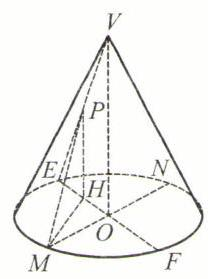
\includegraphics[width=0.2\textwidth]{bodyxb/src/bo_d20cdrf7aajc73bfmvhg_157_1239_1856_208_279_0.jpg}
\end{center}


(第 107 题)

$= \dfrac{\sqrt{3}}{2}a$ . 在 Rt $\bigtriangleup {MOH}$ 中, ${MH} = \sqrt{{a}^{2} + {\left( \dfrac{a}{2}\right) }^{2}} = \dfrac{\sqrt{5}}{2}a,\;\therefore \;\tan \theta  = \dfrac{MH}{PH} = \dfrac{\dfrac{\sqrt{5}}{2}a}{\dfrac{\sqrt{3}}{2}a} = \dfrac{\sqrt{15}}{3}$ ,

$\therefore$ 选 B.

108.C 提示: 圆台侧面积公式: $S = {\pi Rl} + {\pi rl} = \pi  \cdot  \left( {7 + 3}\right)  \cdot  \sqrt{{3}^{2} + {\left( 7 - 3\right) }^{2}} = {50\pi }{\mathrm{\;{cm}}}^{2},\therefore$ 选 C.

109. $C$ 提示:由题 ${8\pi } = \pi  \cdot  \left( {r + R}\right)  \cdot  l = \pi  \cdot  2{l}^{2}$ ,即 $l = 2\mathrm{\;{cm}},\therefore$ 选 $C$ .

110. C 提示: 圆台侧面展开扇环圆心角: $\theta  = \dfrac{{2\pi }\left( {R - r}\right) }{l},\theta  = \dfrac{{2\pi }\left\lbrack  {\left( {r + l \cdot  {\cos }_{0}{60}^{ \circ  }}\right)  - r}\right\rbrack  }{l} = \dfrac{{2\pi } \cdot  \dfrac{l}{2}}{l} = \pi$ ,

\begin{center}
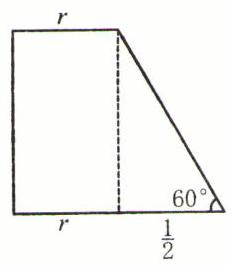
\includegraphics[width=0.2\textwidth]{bodyxb/src/bo_d20cdrf7aajc73bfmvhg_158_1281_212_231_266_0.jpg}
\end{center}


(第 110 题)

$\therefore$ 选 C.

111. B 提示: 圆台上、下底面面积及平行于底面的截面面积分为 ${S}_{1},{S}_{2},{S}_{3}$ ,若截面把圆台的高自上而下分为 $m : n$ 的两段,则 $\sqrt{{S}_{3}} = \dfrac{n\sqrt{{S}_{1}} + m\sqrt{{S}_{2}}}{m + n}$ ,当 $m = n$ 时, $\sqrt{{S}_{3}} = \dfrac{\sqrt{\pi } \cdot  1 + \sqrt{\pi } \cdot  7}{1 + 1} = 4\sqrt{\pi } \Rightarrow$  $S = {16\pi },\therefore$ 选 B.

112. B 提示: 设上、下底半径和母线长分别为 $x,{4x},{5x}$ ,则 ${8}^{2} + {\left( 4x - x\right) }^{2} = {\left( 5x\right) }^{2} \Rightarrow  x = 2$ .

$\therefore S = {\pi Rl} + {\pi rl} = \pi  \cdot  \left( {{4x} + x}\right)  \cdot  {5x} = \pi  \cdot  {10}^{2} = {100\pi }\;\therefore$ 选 B.

\begin{center}
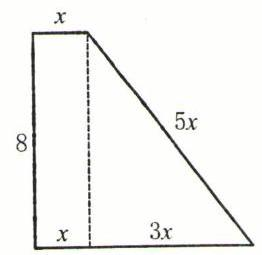
\includegraphics[width=0.2\textwidth]{bodyxb/src/bo_d20cdrf7aajc73bfmvhg_158_1256_553_262_255_0.jpg}
\end{center}


(第 112 题)

113. (1) $\dfrac{512\pi }{3}$ 提示: 设母线长 $l$ ,底面半径 $r$ . 则 ${2\pi r} = \dfrac{6}{5}\pi  \cdot  l$ ,得 $r = \dfrac{3}{5}l$ ,则 $h = \sqrt{{l}^{2} - {r}^{2}} =$

$\sqrt{{l}^{2} - {\left( \dfrac{3}{5}l\right) }^{2}} = \dfrac{32}{3}$ ,得 $l = \dfrac{40}{3},r = 8.{S}_{\text{ 表 }} = {\pi rl} + \pi {r}^{2} = \pi  \cdot  8 \cdot  \dfrac{40}{3} + \pi  \cdot  {64} = \dfrac{512}{3}\pi {\mathrm{{cm}}}^{2}$ .

(2) $\dfrac{84\pi }{5}$ 提示: $S = {\pi r}{l}_{1} + {\pi r}{l}_{2} = {\pi r}\left( {{l}_{1} + {l}_{2}}\right)  = \pi  \cdot  \dfrac{3 \times  4}{5} \cdot  \left( {3 + 4}\right)  = \dfrac{84}{5}\pi$ .

(3) $\left( {3 + \sqrt{2}}\right) \pi {a}^{2}$ 提示: $S = \pi {a}^{2} + \pi  \cdot  a \cdot  {AB} + {2\pi a} \cdot  {AC} = \pi {a}^{2} + {\pi a} \cdot  \sqrt{2}a + {2\pi a} \cdot  a = (3 +$  $\sqrt{2})\pi {a}^{2}$ .

114. (1) $\sqrt{2}\pi$ 提示: 设侧面展开扇形的圆心角为 $\alpha$ ,则 $\alpha  \cdot  l = {2\pi } \cdot  l\sin \dfrac{{90}^{ \circ  }}{2}$ ,得 $\alpha  = \sqrt{2}\pi$ .

(2) 12 提示: ${2\pi r} = {l\alpha }$ ,则 ${2\pi r} = {18} \cdot  \dfrac{4}{3}\pi$ ,则 $r = {12}\mathrm{\;{cm}}$ .

(3) $R$ 提示:三个圆锥侧面积分别为 ${S}_{1},{S}_{2},{S}_{2}$ . 底面周长分别为 ${C}_{1},{C}_{2},{C}_{3},{S}_{1} : {S}_{2} : {S}_{3} = 1 : 2 : 3,{C}_{1} : {C}_{2} : {C}_{3} =$  $1 : 2 : 3$ . 又 ${C}_{1} + {C}_{2} + {C}_{3} = {2\pi R},\therefore {r}_{1} + {r}_{2} + {r}_{3} = R$ .

115. (1) $2\sqrt{3}\pi$ 提示: ${S}_{\text{ 侧 }} = {\pi rl} = \pi  \cdot  \sqrt{2} \cdot  \sqrt{{2}^{2} + 2} = 2\sqrt{3}\pi$ .

(2)11 提示: $\dfrac{1}{2} \cdot  \dfrac{\pi }{5} \cdot  {l}^{2} = {10}$ ,得 $l = \dfrac{{10}\sqrt{\pi }}{\pi }$ ,则底面周长 $C = {\alpha l} = \dfrac{\pi }{5} \cdot  \dfrac{{10}\sqrt{\pi }}{\pi } = 2\sqrt{\pi }$

$\therefore \;r = \dfrac{C}{2\pi } = \dfrac{\sqrt{\pi }}{\pi },\;\therefore \;{S}_{\text{ 全 }} = {S}_{\text{ 侧 }} + {S}_{\text{ 底 }} = {10} + \pi {r}^{2} = {10} + 1 = {11}{\mathrm{\;{cm}}}^{2}$ .

(3) $2 : \sqrt{3}$ 提示: $\dfrac{{S}_{\text{ 偶 }}}{{S}_{\text{ 全 }}} = \dfrac{\pi rl}{{\pi rl} + \pi {r}^{2}} = \dfrac{2}{3},l = {2r}$ ,则 $h = \sqrt{{l}^{2} - {r}^{2}} = \sqrt{4{r}^{2} - {r}^{2}} = \sqrt{3}r$ ,则 $\dfrac{d}{h} = \dfrac{2r}{\sqrt{3}r} = \dfrac{2\sqrt{3}}{3}$ .

(4) ${S}_{\text{ 底 }} = {S}_{\text{ 侧 }} \cdot  \cos \theta$ 提示: 设圆锥底面为 $r$ ,则母线 $l = \dfrac{r}{\cos \theta },\dfrac{{S}_{\text{ 底 }}}{{S}_{\text{ 侧 }}} = \dfrac{\pi {r}^{2}}{\pi rl} = \dfrac{\pi {r}^{2}}{\pi  \cdot  r \cdot  \dfrac{r}{\cos \theta }} = \cos \theta$ . 即 ${S}_{\text{ 底 }} = {S}_{\text{ 侧 }} \cdot  \cos \theta$ .

116. (1) $\dfrac{{200}\sqrt{3}}{3}$ 提示:如图, $P$ 为圆维顶点, $O$ 为底面中心,面 ${ABP}$ 为与底面或 ${60}^{ \circ  }$ 角的截面. $\angle {PMO} = {60}^{ \circ  },{PO} = {10}\mathrm{\;{cm}}$ ,

则 ${PM} = \dfrac{{20}\sqrt{3}}{3}\mathrm{\;{cm}},{MO} = \dfrac{{10}\sqrt{3}}{3}\mathrm{\;{cm}}$ ,又 $\angle {AOB} = {120}^{ \circ  }$ ,则 $\angle {MOB} = {60}^{ \circ  }$ , $\therefore {MB} = {10}$ ,

$\therefore \;{S}_{PAB} = \dfrac{1}{2} \cdot  {20} \cdot  \dfrac{{20}\sqrt{3}}{3} = \dfrac{{200}\sqrt{3}}{3}{\mathrm{\;{cm}}}^{2}$ .

\begin{center}
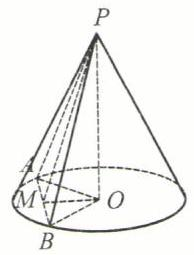
\includegraphics[width=0.2\textwidth]{bodyxb/src/bo_d20cdrf7aajc73bfmvhg_158_617_1733_194_255_0.jpg}
\end{center}


[第 116(1)题]

\begin{center}
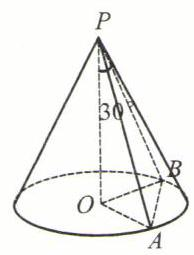
\includegraphics[width=0.2\textwidth]{bodyxb/src/bo_d20cdrf7aajc73bfmvhg_158_961_1726_194_255_0.jpg}
\end{center}


[第 116(2)题]

(2) $4\sqrt{15}$ 提示:如图, $P$ 为圆锥顶点. $O$ 为底面中心, ${AB}$ 为长 $4\mathrm{\;{cm}}$ 的弦. 根据题意, $\angle {AOB} = {60}^{ \circ  }$ . $r = 4\mathrm{\;{cm}}$ ,

则母线长 $l = \dfrac{r}{\sin {30}^{ \circ  }} = 8\mathrm{\;{cm}},\therefore {h}_{\text{ 磁 }} = \sqrt{{8}^{2} - {\left( \dfrac{4}{2}\right) }^{2}} = 2\sqrt{15}\mathrm{\;{cm}},\therefore {S}_{\text{ 截 }} = \dfrac{1}{2} \cdot  4 \cdot  2\sqrt{15} = 4\sqrt{15}{\mathrm{\;{cm}}}^{2}$ ,

(3)18 提示:底面周长 $C = \dfrac{5}{3}\pi  \cdot  6 = {10\pi }\mathrm{{cm}}$ ,则底面半径 $r = \dfrac{C}{2\pi } = 5\mathrm{\;{cm}},\sin \dfrac{\theta }{2} = \dfrac{5}{6}$ ,则 $\theta  > {90}^{ \circ  }$ .

$\therefore \;{S}_{\text{ 截max }} = \dfrac{1}{2}{l}^{2} = \dfrac{1}{2} \times  {6}^{2} = {18}{\mathrm{\;{cm}}}^{2}$ .

117. (1) $\pi$ 提示: 设上、下底面半径及母线长为 $x,{3x},{4x}$ ,则 $\theta  = \dfrac{{2\pi }\left( {R - r}\right) }{l} = \dfrac{{2\pi }\left( {{3x} - x}\right) }{4x} = \pi$ ,即圆心角为 $\pi$ .

(2) $1 : 3$ 提示: $\pi  = \dfrac{{2\pi }\left( {R - r}\right) }{R + r} \Rightarrow  R + r = 2\left( {R - r}\right)$ ,得 $R = {3r}$ ,即 $\dfrac{r}{R} = \dfrac{1}{3}$ .

(3)2 提示: $l = \dfrac{{2\pi }\left( {R - r}\right) }{\theta } = \dfrac{{2\pi }\left( {2 - 1}\right) }{\pi } = 2\mathrm{\;{cm}}$ .

(4)3 提示: ${18\pi } = \pi \left( {R + r}\right) l,{18\pi } = \pi  \cdot  2{l}^{2}$ ,得 $l = 3$ .

118. (1) $\dfrac{4}{3}r$ 提示:由题 $\pi \left( {r + {2r}}\right) l = \pi {r}^{2} + \pi  \cdot  {\left( 2r\right) }^{2},l = \dfrac{5}{3}r$ ,得 $h = \sqrt{{l}^{2} - {\left( 2r - r\right) }^{2}} = \dfrac{4}{3}r$ .

(2) ${35\pi }$ 提示: $\dfrac{{r}_{1}}{{r}_{2}} = \dfrac{2}{5},l = 5,\dfrac{6}{5}\pi  = \dfrac{{2\pi }\left( {{r}_{2} - {r}_{1}}\right) }{l}$ ,得 $\dfrac{6}{5}\pi  = \dfrac{{2\pi }\left( {{r}_{2} - \dfrac{2}{5}{r}_{2}}\right) }{5}$ ,解得 ${r}_{2} = 5,{r}_{1} = 2$ ,

$\therefore \;{S}_{\text{ 侧 }} = \pi \left( {{r}_{1} + {r}_{2}}\right) l = \pi  \cdot  \left( {5 + 2}\right)  \cdot  5 = {35\pi }{\mathrm{\;{cm}}}^{2}$ .

(3) ${25\pi }$ 提示: 设上、下底面半径分别为 $x$ 和 ${4x} \cdot  \dfrac{216}{180} \cdot  \pi  = \dfrac{{2\pi }\left( {{4x} - x}\right) }{\sqrt{{4}^{2} + {\left( 4x - x\right) }^{2}}}$ ,得 $x = 1,\therefore l = \sqrt{{4}^{2} + {\left( 4x - x\right) }^{2}} =$  $5,\;\therefore \;{S}_{\text{ 侧 }} = \pi  \cdot  \left( {x + {4x}}\right)  \cdot  l = \pi  \cdot  5 \cdot  5 = {25\pi }{\mathrm{\;{cm}}}^{2}$ .

\begin{center}
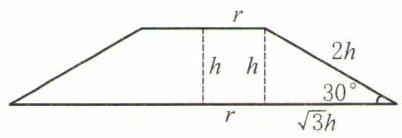
\includegraphics[width=0.3\textwidth]{bodyxb/src/bo_d20cdrf7aajc73bfmvhg_159_1038_825_402_138_0.jpg}
\end{center}


[第 118(4)题]

(4) ${2\pi Q}$ 提示:如图,设上底半径为 $r$ ,高为 $h$ ,则下底半径为 $\left( {r + \sqrt{3}h}\right)$ ,母线长为 ${2h}$ . 又 $Q = \dfrac{1}{2}\left( {{2r} + {2r} + 2\sqrt{3}h}\right)  \cdot  h$ ,即 $\left( {{2r} + \sqrt{3}h}\right) h = Q,\;\therefore \;{S}_{\text{ 侧 }} = \pi  \cdot$  $\left( {r + r + \sqrt{3}h}\right)  \cdot  {2h} = {2\pi } \cdot  \left( {{2r} + \sqrt{3}h}\right)  \cdot  h = {2\pi Q}$ . 即侧面积为 ${2\pi Q}$ .

(5) $\dfrac{5}{4}\pi {a}^{2}$ 提示: $S = 2{S}_{\text{ 台倒 }} + 2{S}_{\text{ 底 }} = 2 \cdot  \pi  \cdot  \left( {\dfrac{a}{4} + \dfrac{a}{2}}\right)  \cdot  \dfrac{a}{2} + 2 \cdot  \pi {\left( \dfrac{a}{2}\right) }^{2} = \dfrac{5}{4}\pi {a}^{2}$ .

(6) $\dfrac{1}{3}S$ 提示:分成的三段底面半径分别为 ${r}_{1},{r}_{2},{r}_{3}$ . 三个圆锥的母线长分别为 ${l}_{1},{l}_{2},{l}_{3}$ ,高分别为 ${h}_{1},{h}_{2},{h}_{3}$ . 侧面分别为 ${S}_{1},{S}_{2},{S}_{3},{r}_{1} : {r}_{2} : {r}_{3} = {l}_{1} : {l}_{2} : {l}_{3} = {h}_{1} : {h}_{2} : {h}_{3} = 1 : 2 : 3$ ,则 ${S}_{1} : {S}_{2} : {S}_{3} :  = \pi {r}_{1}{l}_{1} : \pi {r}_{2}{l}_{3} : \pi {r}_{3}{l}_{3} = 1$  $: 4 : 9$ ,则 ${S}_{1} : \left( {{S}_{2} - {S}_{1}}\right)  : \left( {{S}_{3} - {S}_{2}}\right)  = 1 : 3 : 5,\;\therefore \;{S}_{ \oplus  } = {S}_{2} - {S}_{1} = \dfrac{3}{1 + 3 + 5} \cdot  S = \dfrac{1}{3}S$ .

119. (1) 设圆锥底面半径为 $R$ ,圆柱半径为 $r$ ,圆锥顶点到圆柱上底面的距离为 ${h}_{1}$ ,则 $\dfrac{{2\pi }{r}^{2} + {2\pi rR}}{\pi {R}^{2}} = \dfrac{3}{2}$ ,

$\therefore 3{R}^{2} - {4Rr} - 4{r}^{2} = 0$ ,得 $R = {2r}$ (负已舍). 又 $\dfrac{r}{R} = \dfrac{{h}_{1}}{{h}_{1} + R}$ . 即 $\dfrac{r}{2r} = \dfrac{{h}_{1}}{{h}_{1} + {2r}}$ ,则 ${h}_{1} = {2r}$ ,

$\therefore \;\tan \dfrac{\alpha }{2} = \dfrac{R}{{h}_{1} + R} = \dfrac{2r}{{2r} + {2r}} = \dfrac{1}{2}$ ,则 $\tan \alpha  = \dfrac{4}{3}$ .

(2) $\arcsin \left( \dfrac{{h}^{\prime }}{h}\right)  = \arcsin \dfrac{\sqrt{2}}{2} = \dfrac{\pi }{4}$ .

120. (1) 设 $H$ 为 ${AB}$ 的中点,在 Rt $\bigtriangleup {POH}$ 中, ${PO} = \sqrt{2},\angle {PHO} = {45}^{ \circ  },\therefore {PH} = 2,{OH} = \sqrt{2}$ ,又 ${S}_{\bigtriangleup {PAB}} = 4$ ,

$\therefore {AB} = \dfrac{2 \cdot  4}{2} = 4\mathrm{\;{cm}}$ . 则 $r = \sqrt{O{H}^{2} + B{H}^{2}} = \sqrt{2 + {2}^{2}} = \sqrt{6}\mathrm{\;{cm}},\;\therefore l = \sqrt{{r}^{2} + {h}^{2}} = 2\sqrt{2}\mathrm{\;{cm}}$ , $\therefore {S}_{\text{ 侧 }} = {\pi rl} = 4\sqrt{3}\pi {\mathrm{{cm}}}^{2}$ .

(2)如图, $E,D$ 为截面与底面圆的交点. $O$ 为底面圆心. 过圆锥的高作与截面垂直的平面 ${OAB}$ ,过 ${O作OC} \bot  {AB}$ 于点 $C$ ,则 $\angle {ABO} = {60}^{ \circ  },{OC} = 3\mathrm{\;{dm}}$ ,

\begin{center}
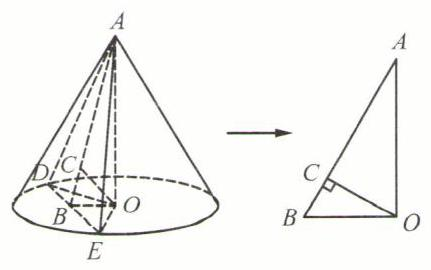
\includegraphics[width=0.3\textwidth]{bodyxb/src/bo_d20cdrf7aajc73bfmvhg_159_1014_1737_431_270_0.jpg}
\end{center}


[第 120(2)题]

$\therefore {BC} = \sqrt{3}\mathrm{{dm}},{BO} = 2\sqrt{3}\mathrm{{dm}},{AO} = 6\mathrm{\;{dm}},{AB} = 4\sqrt{3}\mathrm{{dm}}$ . 又 $\angle {DOE} =$  ${120}^{ \circ  },\;\therefore \angle {EOB} = \angle {DOB} = {60}^{ \circ  }$ ,则 ${OE} = 4\sqrt{3}\mathrm{{dm}} = {OD},{BE} = {BD} =$  $6\mathrm{\;{dm}},{DE} = {BD} + {BE} = {12}\mathrm{\;{dm}}$ . 截面面积: ${S}_{\bigtriangleup {ADE}} = \dfrac{1}{2} \times  {DE} \times  {AB} = \dfrac{1}{2} \times  {12}$  $\times  4\sqrt{3} = {24}\sqrt{3}{\mathrm{{dm}}}^{2}$ ,又 ${OE} = 4\sqrt{3}\mathrm{\;{dm}}$ ,则圆锥侧面弧长为 ${2\pi } \times  4\sqrt{3} = 8\sqrt{3}$  $\pi \mathrm{{dm}}$ . 由勾股定理, ${AE} = \sqrt{A{B}^{2} + B{E}^{2}} = 2\sqrt{21},\;\therefore \;{S}_{\text{ 侧 }} = \dfrac{1}{2} \times  8\sqrt{3}\pi$  $\times  2\sqrt{21} = {24}\sqrt{7}\pi {\mathrm{{dm}}}^{2}.$

121. A 提示: 轴截面顶角即母线最大夹角,设半圆半径 $r$ ,则 ${l}_{半\mathbb{A}} = {\pi r}$ . 即圆锥底面周长为 ${\pi r},\therefore$ 底面直径为 $r$ ,

$\therefore \sin \dfrac{\theta }{2} = \dfrac{\dfrac{r}{2}}{r} = \dfrac{1}{2}$ ,得 $\dfrac{\theta }{2} = \dfrac{\pi }{6}$ ,即 $\theta  = \dfrac{\pi }{3},\;\therefore$ 选 A.

122. B 提示:如图,设母线长为 $a,\because$ 轴截面为直角三角形, $\therefore$ 底面半径 $= {h}_{\text{ 锥 }} = \dfrac{\sqrt{2}}{2}a$ , 则 ${S}_{\text{ 锥侧 }} = \pi  \cdot  \dfrac{\sqrt{2}}{2}a \cdot  a = \dfrac{\sqrt{2}}{2}\pi {a}^{2}$ . 设圆柱底面半径为 $r$ ,高为 $h$ ,则 $\dfrac{r}{\dfrac{\sqrt{2}}{2}a} = \dfrac{\dfrac{\sqrt{2}}{2}a - h}{\dfrac{\sqrt{2}}{2}a}$ ,得 $r = \dfrac{\sqrt{2}}{2}a - h$ .

\begin{center}
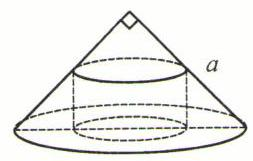
\includegraphics[width=0.2\textwidth]{bodyxb/src/bo_d20cdrf7aajc73bfmvhg_160_1256_270_253_161_0.jpg}
\end{center}


(第 122 题)

① 又 ${2\pi }{r}^{2} + {2\pi r} \cdot  h = \dfrac{\sqrt{2}}{2}\pi {a}^{2}$ ,得 ${2r} \cdot  \left( {r + h}\right)  = \dfrac{\sqrt{2}}{2}{a}^{2}$ ,② 由①②得 $\left\{  \begin{array}{l} r = \dfrac{a}{2}, \\  h = \dfrac{\sqrt{2} - 1}{2}a, \end{array}\right.$

$\therefore \dfrac{h}{{h}_{\text{ 锥 }}} = \dfrac{\dfrac{\sqrt{2} - 1}{2}a}{\dfrac{\sqrt{2}}{2}a} = \dfrac{2 - \sqrt{2}}{2}$ ,

$\therefore$ 选 B.

123. B 提示: 根据题目,轴截面顶角 $\geq  {90}^{ \circ  },\therefore \dfrac{R}{p} = \sin \dfrac{\theta }{2} \geq  \dfrac{\sqrt{2}}{2},\therefore$ 选 B.

124. $C$ 提示: 根据题目,轴截面顶角 $\leq  {90}^{ \circ  }$ ,当轴截面顶角为 ${90}^{ \circ  }$ 时,设母线 $l$ ,则底面半径为 $\dfrac{\sqrt{2}}{2}l$ ,则周长为 $\sqrt{2}{\pi l},\alpha  = \sqrt{2}\pi$ ,此时 $\alpha$ 最大, $\;\therefore \;$ 选 C.

125. D 提示: 设扇形的半径为 $R$ ,圆锥底面半径为 $r$ ,则 $\dfrac{2\pi }{3}R = {2\pi r}$ ,即 $r = \dfrac{R}{3}$ ,则 $\sin \dfrac{\theta }{2} = \dfrac{r}{R} = \dfrac{1}{3},\therefore \cos \theta  = 1 - 2{\sin }^{2}\dfrac{\theta }{2}$  $= \dfrac{7}{9},\;\therefore \;$ 选 D.

126. A 提示: 设原圆锥与截得的圆锥高的比为 $k$ . 截得的圆锥母线长 $l$ ,底面半径为 $r$ ,则原圆锥的母线长为 ${kl}$ ,底面半径为 ${kr}$ . 由题 ${2\pi rl} = {\pi kr} \cdot  {kl},\;\therefore \;{k}^{2} = 2$ ,得 $k = \sqrt{2},\;\therefore \;$ 截得的圆锥与原圆锥高比为 $1 : \sqrt{2}$ . $\therefore$ 选 A.

\begin{center}
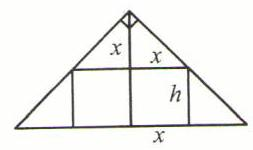
\includegraphics[width=0.2\textwidth]{bodyxb/src/bo_d20cdrf7aajc73bfmvhg_160_1267_1284_253_150_0.jpg}
\end{center}


(第 127 题)

127. C 提示: 如图,设圆柱的高为 $h$ ,圆锥顶点到圆柱上底面距离 $x$ .

由题 ${2\pi }{x}^{2} + {2\pi xh} = \pi \left( {x + h}\right)  \cdot  \sqrt{2}\left( {x + h}\right)$ ,得 $h = \left( {\sqrt{2} - 1}\right) x$ ,

$\therefore$ 圆锥母线长为 $l = \sqrt{2}\left( {x + h}\right)  = {2x}$ ,即 $\dfrac{x}{l} = \dfrac{1}{2}$ ,

$\therefore$ 选 C.

128. $C$ 提示: 如图,设内接正方体棱长为 $a.\dfrac{a}{1} = \dfrac{\dfrac{1}{2} - \dfrac{\sqrt{2}}{2}a}{\dfrac{1}{2}}$ ,得 $a = \sqrt{2} - 1$ ,故选 C.

\begin{center}
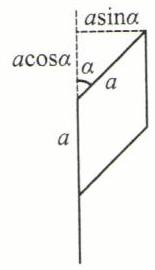
\includegraphics[width=0.2\textwidth]{bodyxb/src/bo_d20cdrf7aajc73bfmvhg_160_931_1629_155_270_0.jpg}
\end{center}


(第 129 题)

\begin{center}
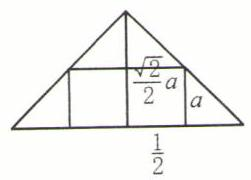
\includegraphics[width=0.2\textwidth]{bodyxb/src/bo_d20cdrf7aajc73bfmvhg_160_555_1724_251_180_0.jpg}
\end{center}


(第 128 题)

129. D 提示: 如图,设菱形的边长为 $a$ ,邻边与旋转轴的夹角为 $\alpha .{S}_{\text{ 表 }} = {2\pi } \cdot  a\sin \alpha  \cdot  a + {2\pi a}\sin \alpha  \cdot  a = {4\pi }{a}^{2}\sin \alpha$ ,又 $Q =$  ${a}^{2}\sin \alpha ,\;\therefore \;{S}_{\text{ 表 }} = {4\pi Q},\;\therefore \;$ 选 D.

130. C 提示: 设两个圆锥底面半径为 ${r}_{1},{r}_{2}$ 母线长为 $l$ . 则 ${2\pi }{r}_{1} + {2\pi }{r}_{2} = {2\pi l}$ ,即 ${r}_{1} + {r}_{2} = l$ . ①

又 $\dfrac{\pi {r}_{1}l}{\pi {r}_{2}l} = \dfrac{1}{2}$ ,即 $\dfrac{{r}_{1}}{{r}_{2}} = \dfrac{1}{2}$ . ② 由①②得 ${r}_{1} = \dfrac{l}{3},{r}_{2} = \dfrac{2l}{3},\therefore$ 高之比为 $\dfrac{\sqrt{{l}^{2} - {r}_{1}^{2}}}{\sqrt{{l}^{2} - {r}_{2}^{2}}} = \dfrac{2\sqrt{10}}{5}$ ,即 $2\sqrt{2} : \sqrt{5}$ ,

$\therefore$ 选 C.

131. 如图, ${S}_{\text{ 表 }} = {2\pi } \cdot  1 \cdot  2 + {2\pi } \cdot  2 \cdot  2\sqrt{2} - {2\pi } \cdot  1 \cdot  \sqrt{2} = {4\pi } + 6\sqrt{2}\pi$ .

132. (1)如图,延长 ${CO}$ 交底面于点 $D$ . ${BD}//{AC}$ ,则 $\angle {PBD}$ 即异面直线 ${AC}$ 与 ${PB}$ 所成角或其补角. ∵ ${AB} = 2$ , $\therefore$  ${OB} = 1.\;\because \;{CD} \bot  {AB},\;\therefore \;{BD} = \sqrt{2}$ . 又 $\angle {APB} = {90}^{ \circ  },\;\therefore \;{PO} = {OB} = 1,\;\therefore \;$ 在 Rt $\bigtriangleup  {POB}$ 中, ${PB} =$  $\sqrt{{1}^{2} + {1}^{2}} = \sqrt{2},$

$\therefore$ 母线 ${PD} = {PB} = \sqrt{2},\therefore \bigtriangleup {PBD}$ 为等边三角形, $\therefore \angle {PBD} = {60}^{ \circ  }$ ,即异面直线 ${AC}$ 和 ${PB}$ 所成角 ${60}^{ \circ  }$ .

(2)取 ${AP}$ 中点 $E$ ,连接 ${CE}$ , ${OE}$ . ${OE} \bot  \dfrac{1}{2}{PB}$ ,又 $\angle {APB} = {90}^{ \circ  }$ , $\therefore {OE} \bot  {AP}$ . $\because {CA} = {CP} = \sqrt{2}$ , $E$ 为 ${AP}$ 中点,

$\therefore {CE} \bot  {AP},\therefore \angle {OEC}$ 即二面角 $B - {PA} - C$ 的平面角. 在 $\bigtriangleup {CEO}$ 中, ${CE} = \dfrac{\sqrt{6}}{2},{OE} = \dfrac{\sqrt{2}}{2},{CO} = 1$ ,

$\therefore \tan \angle {OEC} = \dfrac{OC}{OE} = \sqrt{2}$ .

\begin{center}
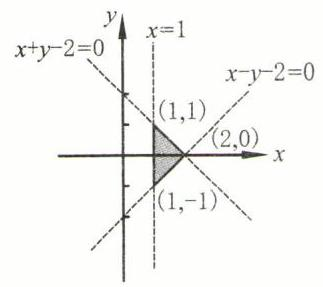
\includegraphics[width=0.2\textwidth]{bodyxb/src/bo_d20cdrf7aajc73bfmvhg_161_235_621_323_287_0.jpg}
\end{center}


(第 131 题)

\begin{center}
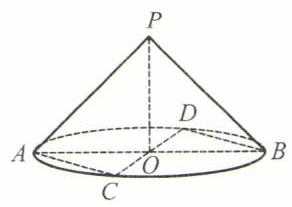
\includegraphics[width=0.2\textwidth]{bodyxb/src/bo_d20cdrf7aajc73bfmvhg_161_640_701_292_207_0.jpg}
\end{center}


(第 132 题)

\begin{center}
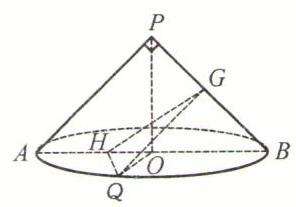
\includegraphics[width=0.2\textwidth]{bodyxb/src/bo_d20cdrf7aajc73bfmvhg_161_1014_697_296_207_0.jpg}
\end{center}


(第 133 题)

133. 如图,过 $Q$ 作 ${QH} \bot  {AB}$ 于点 $H$ ,过 $H$ 作 ${HG} \bot  {PB}$ 于点 $G$ ,连接 ${QG}$ . ‘ $\;{QH} \bot  {AB}$ 且 ${QH} \bot  {PO}$ ,

$\therefore {QH} \bot$ 平面 ${PAB}$ ,又 $\because {HG} \bot  {PB}$ ,由三垂线定理, ${QG} \bot  {PB},\therefore \angle {QGH}$ 即二面角 $A - {PB} - Q$ 平面角.

即 $\tan \angle {QGH} = \dfrac{\sqrt{6}}{3}$ ,不妨设 ${HQ} = \sqrt{6}a,{HG} = {3a}$ . 则 ${BH} = 3\sqrt{2}a$ ,

$\therefore \tan \angle {ABQ} = \dfrac{\sqrt{6}}{3\sqrt{2}} = \dfrac{\sqrt{3}}{3}$ ,即 $\angle {ABQ} = \dfrac{\pi }{6}\;\therefore \angle {AOQ} = 2\angle {ABQ} = \dfrac{\pi }{3}$ .

134. 如图,底面半径 $r = \dfrac{C}{2\pi }$ ,又母线与底面所成的角为 ${60}^{ \circ  },\therefore$ 高 $h = r \cdot  \tan {60}^{ \circ  } = \dfrac{C}{2\pi } \cdot  \sqrt{3} = \dfrac{\sqrt{3}C}{2\pi }$ 则母线 $l = \sqrt{{h}^{2} + {r}^{2}} = \sqrt{{\left( \dfrac{\sqrt{3}C}{2\pi }\right) }^{2} + {\left( \dfrac{C}{2\pi }\right) }^{2}} = \dfrac{C}{\pi }$ ,则 ${h}_{1} = \dfrac{r \cdot  h}{l} = \dfrac{\sqrt{3}C}{4\pi },S = \pi  \cdot  {h}_{1} \cdot  h = \pi  \cdot  \dfrac{\sqrt{3}C}{4\pi }$ . $\dfrac{\sqrt{3}C}{2\pi } = \dfrac{3{C}^{2}}{8\pi }.$

\begin{center}
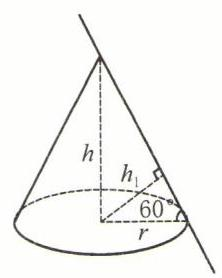
\includegraphics[width=0.2\textwidth]{bodyxb/src/bo_d20cdrf7aajc73bfmvhg_161_1235_1207_222_278_0.jpg}
\end{center}


(第 134 题)

135. 设扇形的半径为 $l$ ,底面半径为 $r$ . 则 $\left\{  \begin{array}{l} l + r + \sqrt{2}r = \sqrt{2}a, \\  {2\pi r} = \dfrac{\pi l}{2}, \end{array}\right.$ 即 $\left\{  \begin{array}{l} r = \dfrac{\sqrt{2}a}{5 + \sqrt{2}}, \\  l = \dfrac{4\sqrt{2}a}{5 + \sqrt{2}}, \end{array}\right.$ 又 ${h}^{2} = {l}^{2} - {r}^{2}$ , 得 $h = \dfrac{\sqrt{30}a}{5 + \sqrt{2}}$ .

136. (1) 如图,设顶点到四棱柱的上底面的距离为 ${h}_{1}$ ,四棱柱底面外接圆半径为 $r$ . 由 $\dfrac{{h}_{1}}{h} =$  $\dfrac{R - r}{R}$ ,得 ${h}_{1} = \dfrac{h\left( {R - r}\right) }{R}$ .

\begin{center}
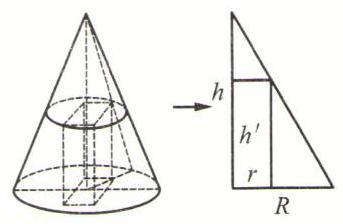
\includegraphics[width=0.2\textwidth]{bodyxb/src/bo_d20cdrf7aajc73bfmvhg_161_1118_1698_343_224_0.jpg}
\end{center}


[第 136(1)题]

$\therefore \;{S}_{\text{ 表 }} = 4{r}^{2} + 4\sqrt{2} \cdot  \dfrac{{rh}\left( {R - r}\right) }{R} = \left( {4 - \dfrac{4\sqrt{2}h}{R}}\right) {r}^{2} + 4\sqrt{2}{rh}$ ,

$\therefore$ 当 $r = \dfrac{4\sqrt{2}h}{\dfrac{8\sqrt{2}h}{R} - 8}$ ,即 $r = \dfrac{Rh}{{2h} - \sqrt{2}R}$ 时, ${S}_{\max } = 4\dfrac{{R}^{2}{h}^{2}}{{\left( 2h - \sqrt{2}R\right) }^{2}} + 4\sqrt{2}\dfrac{Rh}{{2h} - \sqrt{2}R}$ .

$\dfrac{h\left( {R - \dfrac{Rh}{{2h} - \sqrt{2}R}}\right) }{R} = \dfrac{2{h}^{2}R}{\sqrt{2}h - R}.$

(2)如图,设圆柱的底面半径和高分别为 $r$ 和 $h$ . 由 $\dfrac{5 - r}{5} = \dfrac{h}{12}$ ,得 $h = \dfrac{{12}\left( {5 - r}\right) }{5}$ ,则 $S =$  ${2\pi rh} + {2\pi }{r}^{2} = {2\pi r} \cdot  \dfrac{{12}\left( {5 - r}\right) }{5} + {2\pi }{r}^{2} = {2\pi }\left( {-\dfrac{7}{5}{r}^{2} + {12r}}\right)$ . 当 $r = \dfrac{30}{7}\mathrm{\;{cm}}$ 时, ${S}_{\max } =$  $\dfrac{360}{7}\pi {\mathrm{{cm}}}^{2}$ .

\begin{center}
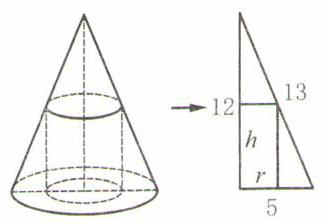
\includegraphics[width=0.2\textwidth]{bodyxb/src/bo_d20cdrf7aajc73bfmvhg_162_1186_112_323_223_0.jpg}
\end{center}


[第 136(2)题]

137. (1) 将圆锥的侧面上由母线 ${PA},{PB}$ 和劣弧 $\overset{⏜}{AB}$ 围成的部分展开成以 $P$ 为圆心的扇形. 在该扇形中,根据题意可知 ${AP} = {PB} = 3,{PC} = \dfrac{3}{2},\overset{⏜}{AB} = \pi ,\angle {BPA} = \dfrac{\pi }{3}$ . 根据余弦定理, $A{C}^{2} = A{P}^{2} + P{C}^{2} - {2PC} \cdot  {AP} \cdot  \cos \angle {BPA} = \dfrac{27}{4},{AC} = \dfrac{3\sqrt{3}}{2}$ ,即最短距离为 $\dfrac{3\sqrt{3}}{2}$ .

(2)如图, $\because {OA} = {10}\mathrm{\;{cm}}$ , $\therefore$ 底面周长 $C = {2\pi } \cdot  {10} = {20\pi }$ . 又 ${PA} = {30}\mathrm{\;{cm}}$ , $\therefore \angle {AP}{A}^{\prime } = \dfrac{C}{PA} = \dfrac{2}{3}\pi$ ,

$\therefore A{A}^{\prime } = 2 \cdot  {30} \cdot  \sin \dfrac{\angle {AP}{A}^{\prime }}{2} = 2 \cdot  {30} \cdot  \sin \dfrac{\pi }{3} = {30}\sqrt{3}\mathrm{\;{cm}}$ . 又 ${PH} = {15}$ ,则 $H$ 为圆锥中最短路线的中点,到底面距离最大. $\therefore H$ 到底面距离为 $\dfrac{1}{2} \cdot  \sqrt{{30}^{2} - {10}^{2}} = {10}\sqrt{2}\mathrm{\;{cm}}$ .

\begin{center}
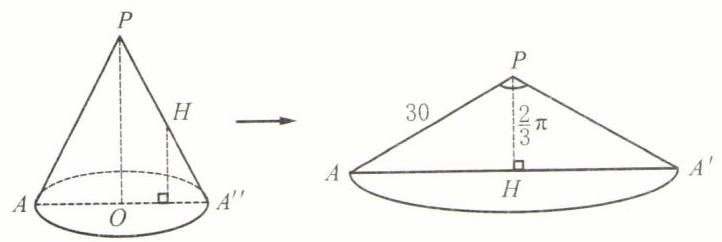
\includegraphics[width=0.6\textwidth]{bodyxb/src/bo_d20cdrf7aajc73bfmvhg_162_475_735_722_242_0.jpg}
\end{center}


[第 137(2)题]

138. B 提示: 如图, ${r}_{1} = \sqrt{\dfrac{{S}_{1}}{\pi }} = \sqrt{\dfrac{5\pi }{\pi }} = \sqrt{5},{r}_{2} = \sqrt{\dfrac{{S}_{2}}{\pi }} = \sqrt{\dfrac{8\pi }{\pi }} = 2\sqrt{2}$ ,设球心到大截面的距离为 $d$ ,设球的半径为 $r$ ,则 ${r}^{2} =$  $5 + {\left( d + 1\right) }^{2} = 8 + {d}^{2},d = 1,r = 3,\;\therefore \;$ 选 B.

\begin{center}
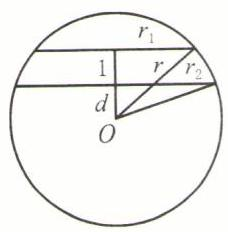
\includegraphics[width=0.2\textwidth]{bodyxb/src/bo_d20cdrf7aajc73bfmvhg_162_407_1179_228_232_0.jpg}
\end{center}


(第 138 题)

\begin{center}
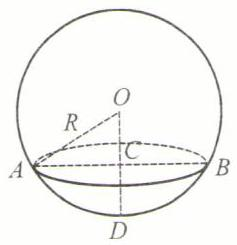
\includegraphics[width=0.2\textwidth]{bodyxb/src/bo_d20cdrf7aajc73bfmvhg_162_723_1162_237_245_0.jpg}
\end{center}


(第 139 题)

\begin{center}
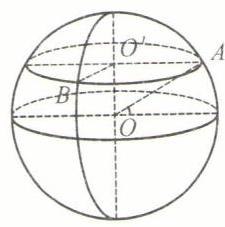
\includegraphics[width=0.2\textwidth]{bodyxb/src/bo_d20cdrf7aajc73bfmvhg_162_1042_1175_225_227_0.jpg}
\end{center}


(第 140 题)

139. $C$ 提示:如图,设球心为 $O$ ,则 ${AB} = {24},{OD}$ 垂直平分 ${AB},C$ 为 ${AB}$ 所在水平截面圆心. 设球的半径为 $R$ ,则在 $\mathrm{{Rt}}$  $\bigtriangleup {AOC}$ 中, $A{O}^{2} = O{C}^{2} + A{C}^{2}$ ,即 ${R}^{2} = {\left( R - 8\right) }^{2} + {12}^{2}$ ,得 $R = {13}\mathrm{\;{cm}}$ , $\therefore$ 选 C.

140.C 提示: 如图, $\because$ 地球半径为 $R$ ,球心为 $O$ ,北纬 ${30}^{ \circ  }$ 圈上 $A,B$ 两点所在圆的圆心为 ${O}^{\prime },\therefore \angle {OA}{O}^{\prime } = {30}^{ \circ  },O{O}^{\prime } =$  $\dfrac{R}{2},{O}^{\prime }A = \dfrac{\sqrt{3}}{2}R$ . 在小圆 $\odot  {O}^{\prime }$ 中 $\angle A{O}^{\prime }B = {120}^{ \circ  },\therefore \overset{⏜}{AB}$ 的长 $= \dfrac{1}{3} \cdot  {2\pi } \cdot  {O}^{\prime }A = \dfrac{1}{3} \cdot  {2\pi } \cdot  \dfrac{\sqrt{3}}{2}R = \dfrac{\sqrt{3}}{3}{\pi R},\therefore$ 选 C.

141. D 提示:当两点是直径的两个端点时,可以作无数个. 当两点不是直径端点时,两点和球心构成一平面,只能作一个大圆, $\therefore$ 选 D.

142. (1) $\dfrac{3}{2}$ 提示: 设球半径为 $R,{S}_{\text{ 球 }} = {4\pi }{R}^{2}$ ,则球的外切圆柱底面半径为 $R$ ,高为 ${2R}.\;\therefore \;{S}_{\text{ 圆柱 }} = {2\pi }{R}^{2} + {2\pi R} \cdot  {2R} =$  ${6\pi }{R}^{2},\;\therefore \;\dfrac{{S}_{\text{ 圆柱 }}}{{S}_{\text{ 球 }}} = \dfrac{{6\pi }{R}^{2}}{{4\pi }{R}^{2}} = \dfrac{3}{2}.$

(2) $4 : 6 : 9$ 提示:由(1)知 $\dfrac{{S}_{\text{ 球 }}}{{S}_{\text{ 圆柱 }}} = \dfrac{2}{3}$ . ① 如图,设等边圆锥轴截面的边长为 $a$ ,

\begin{center}
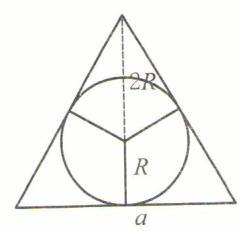
\includegraphics[width=0.2\textwidth]{bodyxb/src/bo_d20cdrf7aajc73bfmvhg_162_1288_1880_242_231_0.jpg}
\end{center}


[第 142(2)题]

则 $\dfrac{\sqrt{3}}{2}a = R + {2R}$ ,即 $a = 2\sqrt{3}R$ ,

$\therefore \dfrac{{S}_{\text{ 球 }}}{{S}_{\text{ 圆锥 }}} = \dfrac{{4\pi }{R}^{2}}{\pi  \cdot  \sqrt{3}R \cdot  2\sqrt{3}R + \pi  \cdot  {\left( \sqrt{3}R\right) }^{2}} = \dfrac{{4\pi }{R}^{2}}{{9\pi }{R}^{2}} = \dfrac{4}{9}$ .②

$\therefore$ 由①②. ${S}_{\text{ 球 }} : {S}_{\text{ 圆柱 }} : {S}_{\text{ 圆锥 }} = 4 : 6 : 9$ ,

(3) $\sqrt{3}a$ 提示: $\because$ 球心到三个墙面的距离均为 $a$ ,

\begin{center}
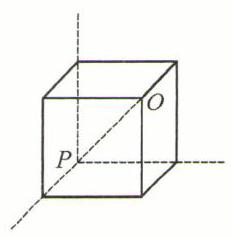
\includegraphics[width=0.2\textwidth]{bodyxb/src/bo_d20cdrf7aajc73bfmvhg_163_1228_114_231_236_0.jpg}
\end{center}


[第 142(3)题]

$\therefore$ 球心 $O$ 到墙角顶点 $P$ 的距离可看成正方体对角线长,即 ${OP} = \sqrt{3{a}^{2}} = \sqrt{3}a$ ,即球心与墙角顶点距离为 $\sqrt{3}a$ .

143. (1) $\dfrac{a}{3}$ 提示: 如图,设内切球半径为 $R,{3R} = \dfrac{\sqrt{3}}{2}a$ ,即 $R = \dfrac{\sqrt{3}}{6}a$ . 设内接正方体的棱长为 $b$ ,则 ${b}^{2}$  $+ {\left( \sqrt{2}b\right) }^{2} = {\left( 2R\right) }^{2}$ ,得 $b = \dfrac{2\sqrt{3}}{3}R = \dfrac{2\sqrt{3}}{3} \cdot  \dfrac{\sqrt{3}}{6}a = \dfrac{a}{3}$ ,即内接正方体的棱长为 $\dfrac{a}{3}$ .

(2) ${9\pi }$ 提示:设长方体同顶点三边长分别为 $a,b,c,{ab} = \sqrt{3},{bc} = \sqrt{5},{ac} = \sqrt{15} \Rightarrow  a = \sqrt{3},b = 1$ , $c = \sqrt{5},\;\therefore \;$ 对角线 $l = \sqrt{{a}^{2} + {b}^{2} + {c}^{2}} = 3,\;\therefore \;R = \dfrac{l}{2} = \dfrac{3}{2},\;\therefore \;S = {4\pi }{R}^{2} = {9\pi }$ .

\begin{center}
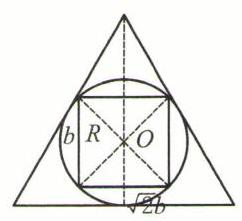
\includegraphics[width=0.2\textwidth]{bodyxb/src/bo_d20cdrf7aajc73bfmvhg_163_1217_411_242_221_0.jpg}
\end{center}


[第 143(1)题]

(3) ${3\pi }{a}^{2}$ 提示: ${PA},{PB},{PC}$ 可看成是正方体的一个顶点发出的三条棱. 所以过空间四个点 $P,A,B,C$ 的球即棱长为 $a$ 的正方体的外接球.

$\therefore R = \dfrac{\sqrt{3}a}{2},\;\therefore S = {4\pi }{R}^{2} = {4\pi } \cdot  {\left( \dfrac{\sqrt{3}a}{2}\right) }^{2} = {3\pi }{a}^{2}$ ,即球面面积为 ${3\pi }{a}^{2}$ .

144. D 提示: $\because {AB} = {BC} = {CA} = 2,\therefore \bigtriangleup {ABC}$ 的外接圆半径为 $r = \dfrac{2\sqrt{3}}{3}$ ,设球的半径为 $R$ ,则 ${R}^{2} - {\left( \dfrac{1}{2}R\right) }^{2} = \dfrac{4}{3}$ ,得 ${R}^{2} = \dfrac{16}{9}$ , $\therefore R = \dfrac{4}{3}$ , $\therefore S = {4\pi }{R}^{2} = \dfrac{64\pi }{9}$ , $\therefore$ 选 D.

145. B 提示: 构造以 ${QA},{QB},{QC}$ 为同一个顶点上三条棱的长方体,已知的球为长方体外接球,则 $Q{A}^{2} + Q{B}^{2} + Q{C}^{2} =$  ${\left( 2R\right) }^{2} = 4{R}^{2},\;\therefore \;$ 选 B.

146. A 提示: 设圆锥母线与底面所成的角为 $\alpha$ ,球的半径为 $R$ ,则 $\cos \alpha  = \dfrac{1}{3}$ ,得 $\cot \alpha  = \dfrac{\sqrt{2}}{4}$ ,圆锥底面半径 $r$  $= {4R}\cot \alpha  = \sqrt{2}R$ ,母线长 $l = {3r} = 3\sqrt{2}R$ , $\therefore \dfrac{{S}_{\text{ 圆锥全 }}}{{S}_{\text{ 球 }}} = \dfrac{\pi {\left( \sqrt{2}R\right) }^{2} + \pi \sqrt{2}R \cdot  3\sqrt{2}R}{{4\pi }{R}^{2}} = 2$ ,

\begin{center}
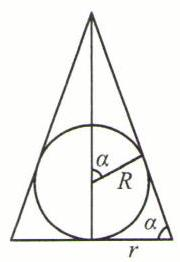
\includegraphics[width=0.2\textwidth]{bodyxb/src/bo_d20cdrf7aajc73bfmvhg_163_1279_904_180_262_0.jpg}
\end{center}


(第 146 题)

$\therefore$ 选 A.

147. D 提示: 四球心组成棱长为 ${2R}$ 的正四面体的四个顶点,则该正四面体的高 $h =$  $\sqrt{{2}^{2}{R}^{2} - {\left( 2 \cdot  \dfrac{\sqrt{3}}{3}\right) }^{2}{R}^{2}} = \dfrac{2\sqrt{6}}{3}R$ . 而第四个球最高点到第四个球球心的距离为 $R$ ,且三个球心到桌面都为 $R,\therefore$ 第四个球最高点到桌面的距离为 $\left( {2 + \dfrac{2\sqrt{6}}{3}}\right) R.\therefore$ 选 D.

148. (1) $7\sqrt{30}\pi$ 提示:如图, ${AH} = 7\mathrm{\;{cm}},{OA} = {OC} = 5\mathrm{\;{cm}}$ ,则 ${OH} = 2\mathrm{\;{cm}}$ ,在 $\mathrm{{Rt}} \bigtriangleup  {OHC}$ 中,

\begin{center}
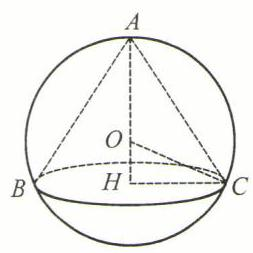
\includegraphics[width=0.2\textwidth]{bodyxb/src/bo_d20cdrf7aajc73bfmvhg_163_1204_1300_253_253_0.jpg}
\end{center}


[第 148(1)题]

${CH} = \sqrt{{5}^{2} - {2}^{2}} = \sqrt{21}\mathrm{\;{cm}},$

$\therefore \;{S}_{\text{ 圆锥侧 }} = \pi  \cdot  \sqrt{21} \cdot  \sqrt{{21} + {7}^{2}} = 7\sqrt{30}\pi {\mathrm{\;{cm}}}^{2}$ .

(2) ${4\pi Rr}$ 提示: 圆台母线长 $l = r + R$ ,则圆台内切球的直径即圆台的高 $\sqrt{{\left( r + R\right) }^{2} - {\left( R - r\right) }^{2}} = 2\sqrt{Rr},\;\therefore$ 圆台内切球的半径为 $\sqrt{Rr},\;\therefore S = {4\pi Rr}$ .

149. ${20}\sqrt{2}\mathrm{\;{cm}}$ 提示: ${12}^{2} + {16}^{2} = {20}^{2},\;\therefore$ 这三点构成直角三角形,

$\therefore$ 球心到三点平面的距离 ${d}^{2} = {30}^{2} - {\left( \dfrac{20}{2}\right) }^{2} = {800}$ ,即 $d = \sqrt{800} = {20}\sqrt{2}\mathrm{\;{cm}}$ .

150. (1) 如图, ${4\pi }{R}^{2} = {36\pi },R = 3$ ,大球半径为 3,即 ${AO} = {OC} = 3$ . 设三棱锥棱长为 $a$ ,则 ${CH} = \dfrac{\sqrt{3}}{2}a \cdot  \dfrac{2}{3} = \dfrac{\sqrt{3}}{3}a$ ,则 ${AH} =$  $\sqrt{{a}^{2} - {\left( \dfrac{\sqrt{3}}{3}a\right) }^{2}} = \dfrac{\sqrt{6}}{3}a,{OH} = \dfrac{\sqrt{6}}{3}a - 3$ . 在 Rt $\bigtriangleup {OHC}$ 中, $O{H}^{2}$  $+ H{C}^{2} = O{C}^{2}$ ,即 ${\left( \dfrac{\sqrt{6}}{3}a - 3\right) }^{2} + {\left( \dfrac{\sqrt{3}}{3}a\right) }^{2} = {3}^{2}$ ,得 $a = 2\sqrt{6},h =$  $\dfrac{\sqrt{6}}{3}a = 4$

\begin{center}
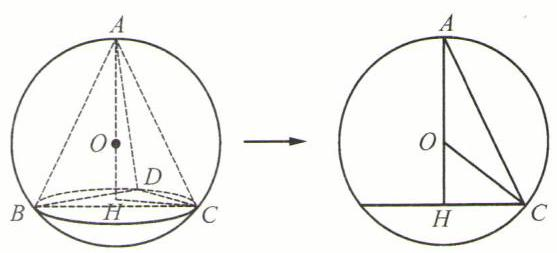
\includegraphics[width=0.4\textwidth]{bodyxb/src/bo_d20cdrf7aajc73bfmvhg_163_904_1644_557_253_0.jpg}
\end{center}


[第 150(1)题]

(2)设正方体棱长为 $a$ ,球半径为 $R$ ,半球与内接正方体补充成一个球和内接长方形,则由长方体对角线性质: ${\left( 2R\right) }^{2} =$  ${a}^{2} + {a}^{2} + {\left( 2a\right) }^{2}$ ,即 $R = \dfrac{\sqrt{6}}{2}a$ . $\;\therefore \;{S}_{\text{ 半球面 }} = \dfrac{1}{2} \cdot  {4\pi }{R}^{2} = {3\pi }{a}^{2},{S}_{\text{ 正方体 }} = 6{a}^{2}$ ,则 $\dfrac{{S}_{\text{ 半球面 }}}{{S}_{\text{ 正方体 }}} = \dfrac{{3\pi }{a}^{2}}{6{a}^{2}} = \dfrac{\pi }{2}$ .

(3)如图,设圆锥底面半径为 $r$ ,母线长 $R$ ,高 $h$ ,则 ${S}_{\text{ 侧 }} = \pi  \cdot  r \cdot  R$ , ${S}_{\text{ 底 }} = \pi  \cdot  {r}^{2}$ , $\therefore \dfrac{{S}_{\text{ 侧 }}}{{S}_{\text{ 底 }}} =$  $\dfrac{\pi rR}{\pi {r}^{2}} = \dfrac{R}{r} = \dfrac{1}{\cos \theta }$ . 设内切球半径为 $a$ ,则 $\dfrac{a}{r} = \tan \dfrac{\theta }{2},{S}_{\text{ 球 }} = {4\pi }{a}^{2}$ ,则由 $\dfrac{{S}_{\text{ 侧 }} + {S}_{\text{ 底 }}}{{S}_{\text{ 球 }}} = \pi  \cdot  r \cdot  \dfrac{R + r}{{4\pi }{a}^{2}}$  $= 2$ ,得 $r\left( {R + r}\right)  = 8{a}^{2},\dfrac{R}{r} + 1 = 8{\left( \dfrac{a}{r}\right) }^{2} = 8{\tan }^{2}\left( \dfrac{\theta }{2}\right)$ ,则 $\cos \theta  = \dfrac{r}{R} = \dfrac{1}{3}$ ,即 $\dfrac{{S}_{\text{ 侧 }}}{{S}_{\text{ 底 }}} = 3$ .

\begin{center}
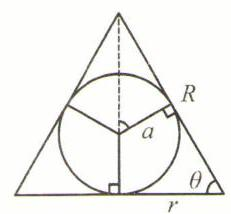
\includegraphics[width=0.2\textwidth]{bodyxb/src/bo_d20cdrf7aajc73bfmvhg_164_1284_112_231_214_0.jpg}
\end{center}


[第 150(3)题]

151. 如图,作 ${OE}\bot {AP}$ 于点 $E$ ,则 $\angle {POE} = \angle {PAH} = \alpha$ . 又 ${ABCD}$ 为边长 $a$ 的正方形,

$\therefore {AH} = \dfrac{\sqrt{2}}{2}a,\therefore {AP} = \dfrac{\sqrt{2}a}{2\cos \alpha }$ ,则 ${PE} = \dfrac{\sqrt{2}a}{4\cos \alpha }.\therefore {OP} = \dfrac{PE}{\sin \alpha } = \dfrac{\sqrt{2}a}{4\sin \alpha \cos \alpha }$ ,即 $R = \dfrac{\sqrt{2}a}{4\sin \alpha \cos \alpha }$ ,

$\therefore \;S = {4\pi }{R}^{2} = {4\pi } \cdot  \dfrac{1}{8} \cdot  \dfrac{{a}^{2}}{{\sin }^{2}\alpha {\cos }^{2}\alpha } = \dfrac{{2\pi }{a}^{2}}{{\sin }^{2}{2\alpha }}$ .

\begin{center}
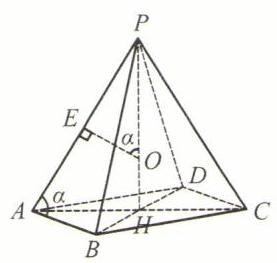
\includegraphics[width=0.2\textwidth]{bodyxb/src/bo_d20cdrf7aajc73bfmvhg_164_507_549_277_263_0.jpg}
\end{center}


(第 151 题)

\begin{center}
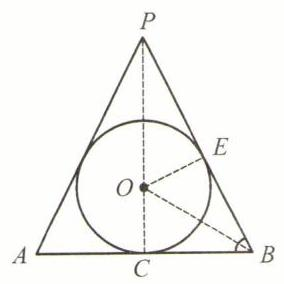
\includegraphics[width=0.2\textwidth]{bodyxb/src/bo_d20cdrf7aajc73bfmvhg_164_892_525_284_284_0.jpg}
\end{center}


[第 152(1)题]

152. (1) 证明: 设母线长为 $l$ ,圆锥底面半径 $r,l = {PB} = {PE} + {EB} = {PE} + {BC} = {OE} \cdot  \tan {2\alpha } + \dfrac{OC}{\tan \alpha } = \dfrac{2\tan \alpha }{1 - {\tan }^{2}\alpha } \cdot  R + \dfrac{1}{\tan \alpha } \cdot  R$

$= \dfrac{1 + {\tan }^{2}\alpha }{\tan \alpha \left( {1 - {\tan }^{2}\alpha }\right) }R,\;\therefore \;{S}_{\text{ 全 }} = \pi {r}^{2} + {\pi rl} = {\pi r}\left( {r + l}\right)  = \dfrac{\pi R}{\tan \alpha } \cdot  \dfrac{2R}{\tan \alpha \left( {1 - {\tan }^{2}\alpha }\right) } = \dfrac{{2\pi }{R}^{2}}{{\tan }^{2}\alpha \left( {1 - {\tan }^{2}\alpha }\right) }.$

( 2 )由( 1 )知要使 ${S}_{\text{ 全 }}$ 最小,即 ${\tan }^{2}\alpha  \cdot  \left( {1 - {\tan }^{2}\alpha }\right)$ 最大,而 ${\tan }^{2}\alpha  \cdot  \left( {1 - {\tan }^{2}\alpha }\right)  \leq  {\left( \dfrac{{\tan }^{2}\alpha  + 1 - {\tan }^{2}\alpha }{2}\right) }^{2} = \dfrac{1}{4}$ . $\therefore$ 当且仅当 ${\tan }^{2}\alpha  = 1 - {\tan }^{2}\alpha$ ,即 $\tan \alpha  = \dfrac{\sqrt{2}}{2}$ 时, ${S}_{\text{ 全 }}$ 最小为 ${8\pi }{R}^{2}$ .

153. (1) 如图,设圆台底面半径分别为 ${r}_{1},{r}_{2}$ ,内切球半径为 $r$ ,则高 $h = {2r}$ ,则 ${\left( 2r\right) }^{2} + {\left( {r}_{2} - {r}_{1}\right) }^{2} =$  ${\left( {r}_{1} + {r}_{2}\right) }^{2}$ ,即 ${r}_{1}{r}_{2} = {r}^{2}$ ,即 ${d}_{1}{d}_{2} = 4{r}^{2} = {h}^{2}$ 得证.

\begin{center}
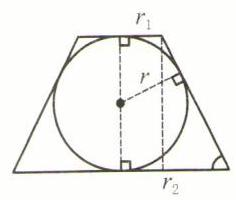
\includegraphics[width=0.2\textwidth]{bodyxb/src/bo_d20cdrf7aajc73bfmvhg_164_1287_1163_236_200_0.jpg}
\end{center}


[第 153(1)题]

(2)设上下底半径分别为 ${r}_{1},{r}_{2}$ ,球半径为 $r$ ,高为 ${2r}$ ,则 ${r}_{2} = r \cdot  \cot \dfrac{\alpha }{2},{r}_{1} = r \cdot  \tan \dfrac{\alpha }{2}$ .

$\therefore$ 母线长 $l = \dfrac{2r}{\sin \alpha }$ ,

$\therefore {S}_{\text{ 圆台侧 }} = \pi \left( {{r}_{1} + {r}_{2}}\right) l = \dfrac{{4\pi }{r}^{2}}{{\sin }^{2}\alpha },\;\therefore \;\dfrac{{S}_{\text{ 圆台侧 }}}{{S}_{\text{ 球 }}} = \dfrac{\dfrac{{4\pi }{r}^{2}}{{\sin }^{2}\alpha }}{{4\pi }{r}^{2}} = \dfrac{1}{{\sin }^{2}\alpha }$ .

(3)设圆台母线和底面所面角为 $\theta$ ,则由(2)的结论,得 $\sin \theta  = \dfrac{\sqrt{3}}{2} \Rightarrow  \theta  = \dfrac{\pi }{3}$ .

(4) 设上下底面半径 ${r}_{1},{r}_{2}\left( {{r}_{1} < {r}_{2}}\right)$ ,则 $\left\{  \begin{array}{l} \dfrac{\pi {r}_{1}^{2} + \pi {r}_{2}^{2} + \pi {\left( {r}_{1} + {r}_{2}\right) }^{2}}{{4\pi }{R}^{2}} = \dfrac{p}{1}, \\  {\left( 2R\right) }^{2} + {\left( {r}_{2} - {r}_{1}\right) }^{2} = {\left( {r}_{1} + {r}_{2}\right) }^{2}, \end{array}\right.$ 得 $\left\{  \begin{array}{l} {r}_{1} = \dfrac{R}{2}\left( {\sqrt{{2p} + 1} - \sqrt{{2p} - 3}}\right) , \\  {r}_{2} = \dfrac{R}{2}\left( {\sqrt{{2p} + 1} + \sqrt{{2p} - 3}}\right) . \end{array}\right.$

154. 如图,设圆锥高 $h$ ,母线长 $l = \sqrt{{R}^{2} + {h}^{2}}$ ,则球半径 $r = \dfrac{hR}{l} = \dfrac{hR}{\sqrt{{R}^{2} + {h}^{2}}}$ . 又 ${S}_{\text{ 圆锥全 }} = {S}_{\text{ 球 }}$ ,即 $\pi  \cdot  R$

\begin{center}
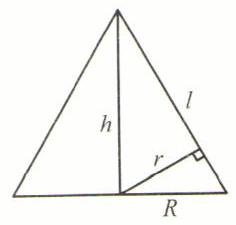
\includegraphics[width=0.2\textwidth]{bodyxb/src/bo_d20cdrf7aajc73bfmvhg_164_1296_1716_236_225_0.jpg}
\end{center}


(第 154 题)

\begin{itemize}
\item $\sqrt{{R}^{2} + {h}^{2}} + \pi {R}^{2} = {4\pi } \cdot  {\left( \dfrac{hR}{\sqrt{{R}^{2} + {h}^{2}}}\right) }^{2}$ ,即 ${\left( {h}^{2} + {R}^{2}\right) }^{3} = {R}^{2} \cdot  {\left( 3{h}^{2} - {R}^{2}\right) }^{2}$ ,即 ${h}^{4} - 6{h}^{2}{R}^{2} + 9{R}^{4}$  $= 0$ ,即 ${\left( {h}^{2} - 3{R}^{2}\right) }^{2} = 0$ ,即 ${h}^{2} = 3{R}^{2}.\;\therefore$ 母线 $l = \sqrt{{R}^{2} + {h}^{2}} = \sqrt{{R}^{2} + 3{R}^{2}} = {2R},\;\therefore \;{S}_{\text{ 圆锥全 }}$  $= {\pi Rl} + \pi {R}^{2} = \pi  \cdot  R \cdot  {2R} + \pi {R}^{2} = {3\pi }{R}^{2}.$
\end{itemize}

155. A 提示: 设底面边长为 $x$ ,高为 $h$ ,则 $P = {x}^{2},Q = \sqrt{2}{xh},\therefore V = {x}^{2} \cdot  h = \dfrac{Q}{\sqrt{2}} \cdot  \sqrt{P} = \dfrac{\sqrt{2P}}{2}Q$ , $\therefore$ 选 A.

156. C 提示: 如图,显然 $\dfrac{{V}_{ \Uparrow  }}{{V}_{ \uparrow  }} = \dfrac{1}{3},\therefore$ 选 C.

\begin{center}
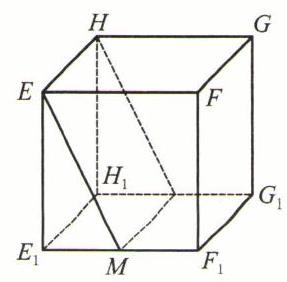
\includegraphics[width=0.2\textwidth]{bodyxb/src/bo_d20cdrf7aajc73bfmvhg_165_1163_119_287_282_0.jpg}
\end{center}


(第 156 题)

157. A 提示: $S = \pi {r}^{2},r = \sqrt{\dfrac{S}{\pi }}.T = {2rh},{rh} = \dfrac{T}{2}.\;\therefore V = \pi {r}^{2} \cdot  h = \pi  \cdot  \dfrac{T}{2} \cdot  \sqrt{\dfrac{S}{\pi }} = \dfrac{T}{2}$ . $\sqrt{S\pi }$ . $\therefore$ 选 A.

158. D 提示: 等边圆柱为母线和底面直径相等的圆柱, $d = h = \sqrt{Q},\therefore V = \dfrac{\pi {d}^{2}}{4} \cdot  h = \dfrac{\pi }{4}Q$ . $\sqrt{Q},\;\therefore \;$ 选 D.

159. B 提示: ${OD}$ 为内圆柱底面半径, ${OA}$ 为外圆柱底面半径,在 $\mathrm{{Rt}} \bigtriangleup  {OAD}$ 中, $\angle {OAD} = {30}^{ \circ  }$ , $\therefore \dfrac{OD}{OA} = \dfrac{1}{2},\;\therefore \dfrac{{V}_{\text{ 内 }}}{{V}_{\text{ 外 }}} = \dfrac{\pi  \cdot  O{D}^{2} \cdot  h}{\pi  \cdot  O{A}^{2} \cdot  h} = \dfrac{1}{4}.\;\therefore \;$ 选 B. 160. D 提示: 该圆柱有两种可能: $\text{ ① }{\pi d} = 6,h = 4$ ,则 $V = \pi  \cdot  \dfrac{{d}^{2}}{4} \cdot  h = \dfrac{36}{\pi }$ . $\text{ ② }{\pi d} = 4,h = 6$ ,则 $V = \pi  \cdot  \dfrac{{d}^{2}}{4} \cdot  h = \dfrac{24}{\pi }$ . $\therefore$ 选 D. 161. C 提示: 正六棱柱底面,最长对角线长 $4\sqrt{3}\mathrm{\;{cm}},\therefore$ 高为 $\sqrt{{8}^{2} - {\left( 4\sqrt{3}\right) }^{2}} = 4\mathrm{\;{cm}},\therefore V = \dfrac{\sqrt{3}}{4} \cdot  {\left( 2\sqrt{3}\right) }^{2} \cdot  6 \cdot  4 = {72}\sqrt{3}$  ${\mathrm{{cm}}}^{3},\;\therefore \;$ 选 C.

162. (1) $\sqrt{6}$ 提示:设长方体同一顶点三条棱长 $a,b,c$ ,则 ${ab} = \sqrt{2},{bc} = \sqrt{3},{ac} = \sqrt{6},\;\therefore \;{\left( abc\right) }^{2} = \sqrt{2} \cdot  \sqrt{3} \cdot  \sqrt{6} = 6$ , $\therefore V = {abc} = \sqrt{6}$ . (2)27 提示:设原正方体棱长为 $a\mathrm{\;{cm}}$ ,则 ${\left( a + 2\right) }^{3} - {a}^{3} = {98}$ , $\therefore a = 3$ (负值舍), $\therefore V = {a}^{3} = {27}{\mathrm{\;{cm}}}^{3}$ . (3) $\sqrt{{S}_{1}{S}_{2}{S}_{3}}$ 提示:设三条棱长分别为 $a,b,c$ ,则 ${ab} = {S}_{1},{ac} = {S}_{2},{ab} = {S}_{3},\;\therefore \;{\left( abc\right) }^{2} = {S}_{1} \cdot  {S}_{2} \cdot  {S}_{3}$ , $\therefore V = {abc} = \sqrt{{S}_{1}{S}_{2}{S}_{3}}$ . 163. (1) $\dfrac{\sqrt{2}}{2}\pi {a}^{3}$ 提示: $d = h = \sqrt{2{a}^{2}} = \sqrt{2}a,\therefore S = \pi  \cdot  {\left( \dfrac{d}{2}\right) }^{2} = \dfrac{\pi }{2}{a}^{2},\therefore V = {Sh} = \dfrac{\pi }{2}{a}^{2} \cdot  \sqrt{2}a = \dfrac{\sqrt{2}}{2}\pi {a}^{3}$ .

\begin{center}
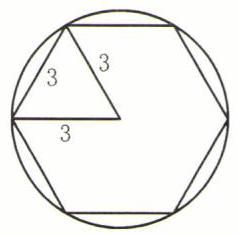
\includegraphics[width=0.2\textwidth]{bodyxb/src/bo_d20cdrf7aajc73bfmvhg_165_501_1080_238_235_0.jpg}
\end{center}


[第 163(2)题]

\begin{center}
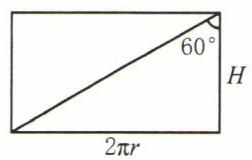
\includegraphics[width=0.2\textwidth]{bodyxb/src/bo_d20cdrf7aajc73bfmvhg_165_845_1154_252_160_0.jpg}
\end{center}


[第 163(6)题]

(2) ${81}\sqrt{3}$ 提示:等边圆柱为轴截面为正方形的圆柱,由题 $d = h = \sqrt{36} = 6\mathrm{\;{cm}}$ ,则圆柱内接正六棱柱的底面截图如图所示, $V = \left( {\dfrac{\sqrt{3}}{4} \cdot  {3}^{2} \cdot  6}\right)  \cdot  6 = {81}\sqrt{3}{\mathrm{\;{cm}}}^{3}$ .

(3) ${r}^{2}h$ 提示:以圆柱轴截面为一个侧面,则该内接三棱柱的底面三角形有一边是圆柱底面圆的直径,此时作内接三角形面积最大为等腰直角三角形. 相应的, ${V}_{\max } = \dfrac{1}{2} \cdot  {2r} \cdot  r \cdot  h = {r}^{2}h$ .

(4) $\dfrac{2{b}^{2}}{{a}^{2}}$ 提示: $\left\{  \begin{array}{l} {2\pi r} \cdot  h = \pi {a}^{2}, \\  \pi {r}^{2}h = \pi {b}^{2}, \end{array}\right.$ ① $\dfrac{\text{ ② }}{\text{ ① }}$ ,得 $r = \dfrac{2{b}^{2}}{{a}^{2}}$ .

(5) $2 : 1$ 提示: 圆柱 1 中, ${C}_{\text{ 底 }} = {2\pi r},{S}_{\text{ 底 }} = \pi {r}^{2},h = a$ . 圆柱 2 中, ${C}_{\text{ 底 }} = {2\pi R},{S}_{\text{ 底 }} = \pi {R}^{2},h = b$ ,则 $\left\{  {\begin{array}{l} b = {2\pi r}, \\  a = {2\pi R}, \\  {2\pi }{r}^{2}a = \pi {R}^{2}b, \end{array}\text{ 得 }a}\right.$ : $b = 2 : 1$ . (6) $\dfrac{3{H}^{3}}{4\pi }$ 提示: 如图为该圆柱侧面展开图,设圆柱底面半径为 $r$ ,则 ${2\pi r} = \sqrt{3}H$ ,即 $r = \dfrac{\sqrt{3}H}{2\pi },\therefore V = \pi {r}^{2} \cdot  H$  $= \dfrac{3{H}^{3}}{4\pi }$ .

164. (1) $V = S \cdot  h = \left( {\dfrac{1}{2} \cdot  3 \cdot  4}\right) \left( {{10} \cdot  \sin {45}^{ \circ  }}\right)  = 6 \cdot  5\sqrt{2} = {30}\sqrt{2}{\mathrm{\;{cm}}}^{3}$ .

(2)设侧棱长为 $y\mathrm{\;{cm}}$ ,侧面 $A{A}_{1}{B}_{1}B$ 中, $A{A}_{1}$ 上的高为 ${8x}\mathrm{\;{cm}}$ ,侧面 $A{A}_{1}{C}_{1}C$ 中 $A{A}_{1}$ 上的高为 ${5x}\mathrm{\;{cm}}$ .

$\because$ 侧面 $A{A}_{1}{B}_{1}B$ 与侧面 $A{A}_{1}{C}_{1}C$ 成 ${60}^{ \circ  }$ ,

$\therefore$ 由余弦定理得 $B{B}_{1}{C}_{1}C$ 中侧棱上的高 $h = \sqrt{{64}{x}^{2} + {25}{x}^{2} - 2 \cdot  {8x} \cdot  {5x} \cdot  \dfrac{1}{2}} = {7x}.\;\because$ 棱柱的侧面积为 ${60}{\mathrm{\;{cm}}}^{2}$ ,体积为 ${15}\sqrt{3}{\mathrm{\;{cm}}}^{3},\therefore \left\{  \begin{array}{l} {5xy} + {8xy} + {7xy} = {60}, \\  \dfrac{1}{2} \cdot  {5x} \cdot  {8x} \cdot  \dfrac{\sqrt{3}}{2}y = {15}\sqrt{3}, \end{array}\right.$ 得 $\left\{  {\begin{array}{l} x = \dfrac{1}{2}, \\  y = 6. \end{array}\;\therefore \;\text{ 侧棱长为 }6\mathrm{\;{cm}}}\right.$ .

165. C 提示: 底面边长为 $\sqrt{S}$ . 一个侧面面积为 $\dfrac{Q}{4}$ ,故斜高 $h = \dfrac{Q}{2\sqrt{S}}$ ,又设棱锥高为 $H,{\left( \dfrac{\sqrt{S}}{2}\right) }^{2} + {H}^{2} = \dfrac{{Q}^{2}}{4S}$ ,得 $H =$  $\dfrac{\sqrt{S\left( {{Q}^{2} - {S}^{2}}\right) }}{2S},V = \dfrac{1}{3}{SH} = \dfrac{1}{6}\sqrt{S\left( {{Q}^{2} - {S}^{2}}\right) },\;\therefore$ 选 C.

166. B 提示:如图,在 $\mathrm{{Rt}} \bigtriangleup  {ABC}_{1}$ 中, $\angle {AC}_{1}B = {30}^{ \circ  }$ ,又 ${AB} = a$ , $\therefore {AC}_{1} = {2a},{BC}_{1} = \sqrt{3}a$ . 又 $\mathrm{{Rt}} \bigtriangleup  {BCC}_{1}$ 中, ${BC} = a$ , $\therefore$  $C{C}_{1} = \sqrt{2}a.\;\therefore \;V = {a}^{2} \cdot  \sqrt{2}a = \sqrt{2}{a}^{3},\;\therefore \;$ 选 B.

\begin{center}
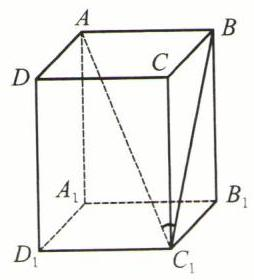
\includegraphics[width=0.2\textwidth]{bodyxb/src/bo_d20cdrf7aajc73bfmvhg_166_476_601_254_280_0.jpg}
\end{center}


(第 166 题)

\begin{center}
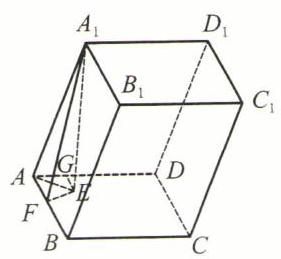
\includegraphics[width=0.2\textwidth]{bodyxb/src/bo_d20cdrf7aajc73bfmvhg_166_839_613_281_259_0.jpg}
\end{center}


(第 167 题)

167. A 提示:如图,设平行六面体为 ${A}_{1}{B}_{1}{C}_{1}{D}_{1} - {ABCD},{A}_{1}A = a,{AB} = b,{AD} = c,\angle {A}_{1}{AB} = \angle {A}_{1}{AD} = \angle {DAB} = {60}^{ \circ  }$ . 作 ${A}_{1}E \bot  {ABCD}$ , $E$ 为垂足. 连接 ${AE}$ ,过 ${A}_{1}$ 作 ${AB}$ , ${AD}$ 的垂线 ${A}_{1}F$ , ${A}_{1}G$ , $F$ 和 $G$ 为垂足. $\;\because \angle {A}_{1}{AB} = \angle {A}_{1}{AD}$ ,

$\therefore {A}_{1}F = {A}_{1}G$ ,且 ${EF}\bot {AD},{EG}\bot {AD}.\therefore E$ 在 $\angle {BAD}$ 的平分线上,即 $\angle {BAE} = {30}^{ \circ  }$ . 在 $\mathrm{{Rt}} \bigtriangleup  {A}_{1}{AF}$ 中, ${A}_{1}A = a$ , $\angle {A}_{1}{AF} = {60}^{ \circ  },\;\therefore \;{AF} = \dfrac{a}{2},{A}_{1}F = \dfrac{\sqrt{3}}{2}a$ . 在 Rt $\bigtriangleup  {AEF}$ 中, ${EF} = {AF} \cdot  \dfrac{\sqrt{3}}{3} = \dfrac{\sqrt{3}}{6}a$ . 在 Rt $\bigtriangleup  {A}_{1}{EF}$ 中, ${A}_{1}E =$  $\sqrt{{A}_{1}{F}^{2} - E{F}^{2}} = \dfrac{\sqrt{6}}{3}a.\;\therefore \;{S}_{▱{ABCD}} = {bc} \cdot  \sin {60}^{ \circ  } = \dfrac{\sqrt{3}}{2}{bc},\;\therefore \;{V}_{\text{ 平行六面体 }} = \dfrac{\sqrt{3}}{2}{bc} \cdot  \dfrac{\sqrt{6}}{3}a = \dfrac{\sqrt{2}}{2}{abc}.\;\therefore \;$ 选 A.

168. (1) $\dfrac{\pi }{4}\dfrac{\sqrt{2}}{16}\pi$ 提示: 设轴截面对角线与底面所成角为 $\alpha ,{S}_{\text{ 侧 }} = \pi  \cdot  \left( {1 \cdot  \cos \alpha }\right)  \cdot  \left( {1 \cdot  \sin \alpha }\right)  = \pi \sin \alpha \cos \alpha  = \dfrac{\pi }{2} \cdot  \sin {2\alpha }$ . 当 ${2\alpha } = \dfrac{\pi }{2}$ ,即 $\alpha  = \dfrac{\pi }{4}$ 时, ${S}_{\text{ 侧max }} = \dfrac{\pi }{2}$ . 此时 $V = \pi {r}^{2} \cdot  h = \pi  \cdot  {\left( \dfrac{\sqrt{2}}{4}\right) }^{2} \cdot  \dfrac{\sqrt{2}}{2} = \dfrac{\sqrt{2}}{16}\pi$ .

(2) $\sqrt{3}$ 提示: $\because$ 侧面 ${AC}{C}_{1}{A}_{1}$ 是矩形, $\therefore {AC} \bot  C{C}_{1}$ . 又 ${AC} \bot  {CB}$ , $\therefore {AC} \bot$ 平面 ${BC}{C}_{1}{B}_{1}$ , $\therefore$ 平面 ${BC}{C}_{1}{B}_{1} \bot$ 平面 ${ABC}$ . 过点 ${B}_{1}$ 作 ${B}_{1}D \bot  {BC}$ ,垂足为 $D$ ,则 ${B}_{1}D \bot$ 平面 ${ABC}$ . 又 ${S}_{{B}_{1}{BC}{C}_{1}} = 2\sqrt{3},\therefore {BC} \cdot  {B}_{1}D =$  $2\sqrt{3}$ ,又 ${S}_{\bigtriangleup {ABC}} = \dfrac{1}{2}{AC} \cdot  {CB} = \dfrac{1}{2}{BC},\;\therefore \;V = {S}_{\bigtriangleup {ABC}} \cdot  {B}_{1}D = \dfrac{1}{2}{BC} \cdot  {B}_{1}D = \dfrac{1}{2} \cdot  2\sqrt{3} = \sqrt{3}$ .

169. (1) 取 ${A}_{1}{B}_{1}$ 中点 $M$ ,连接 ${PM},{C}_{1}M$ ,设正三角形的边长为 $x$ ,则 ${C}_{1}M \bot$ 面 $A{A}_{1}{BB},\therefore \angle {C}_{1}{PM} = {30}^{ \circ  }$ . 由勾股定理有 ${C}_{1}P = \sqrt{{x}^{2} + 4}$ ,且 ${C}_{1}M = \sqrt{3} \cdot  \dfrac{x}{2},{C}_{1}P = 2 \cdot  {C}_{1}M = \sqrt{3}x,\therefore x = \sqrt{2},V = \sqrt{3} \cdot  2 \cdot  \dfrac{3}{4} = \dfrac{3\sqrt{3}}{2}$ .

(2)取 ${AC}$ 中点 $M$ ,连接 ${GM}$ , ${HM}$ . $\because H$ , $G$ 分别为 ${AB}$ , ${A}_{1}{C}_{1}$ 的中点, $\therefore {HM} ⫫ \dfrac{1}{2}{BC}$ , ${GM}//{A}_{1}A$ , $\therefore {GM}$ 上平面 ${ABC},\therefore {GM} \bot  {HM}$ ,在 $\mathrm{{Rt}} \bigtriangleup  {GMH}$ 中, ${HM} = \dfrac{1}{2}{BC},{HG} = 2\mathrm{\;{cm}},\angle {GHM} = {60}^{ \circ  },\therefore {BC} = {2HM} =$  $2 \cdot  1 = 2\mathrm{\;{cm}},{GM} = \sqrt{3}\mathrm{\;{cm}},\;\therefore \;V = \dfrac{\sqrt{3}}{4} \cdot  {2}^{2} \cdot  \sqrt{3} = 3{\mathrm{\;{cm}}}^{3}.$

170. (1) ${S}_{\text{ 侧 }} = \dfrac{\sqrt{2}}{2}b \cdot  a \cdot  2 + {ab} = \left( {\sqrt{2} + 1}\right) {ab},V = \dfrac{\sqrt{3}}{4}{a}^{2} \cdot  \dfrac{\sqrt{3}}{3}b = \dfrac{1}{4}{a}^{2}b$ .

(2)①在面 ${BC}{C}_{1}{B}_{1}$ 内作 ${NP}\bot {BC}$ 于点 $P.\because {BC}{C}_{1}{B}_{1}$ 为正方形, $\therefore {C}_{1}C\bot {BC}$ . 又 ${NP}\bot {BC},\therefore {NP}//$  $C{C}_{1}$ . 在面 ${ABCD}$ 中作 ${MQ}\bot {AB}$ 于点 $Q.\because {AM} = {BN},\angle {MQA} = \angle {NPB} = {90}^{ \circ  },\angle {MAQ} = \angle {NBP} = {45}^{ \circ  }$ ,

$\therefore  \bigtriangleup  {MAQ} \cong   \bigtriangleup  {NBP},\therefore {AQ} = {MQ} = {BP} = {NP},\therefore$ 四边形 ${MQBP}$ 为矩形. $\therefore {MP}//{AB}$ ,且 ${NP}//$  $C{C}_{1},{MP}//{CD},\therefore$ 平面 ${MPN}//$ 平面 ${DC}{C}_{1}{D}_{1},\therefore {MN}//$ 侧面 ${DC}{C}_{1}{D}_{1}$ .

②在 $\bigtriangleup {MNP}$ 中, ${MN} = \dfrac{\sqrt{14}}{4}$ . $\angle {MPN} = {60}^{ \circ  }$ . 又 ${BN} : N{C}_{1} = 1 : 3$ ,设 ${NP} = a$ ,则 $C{C}_{1} = {4a}$ ,即 ${AB} = {4a}$ . 又 ${AQ} =$

${NP} = a$ ,则 ${MP} = {QB} = {3a}$ . 由余弦定理 $\dfrac{{a}^{2} + {\left( 3a\right) }^{2} - M{N}^{2}}{2 \cdot  a \cdot  {3a}} = \cos \angle {MPN}$ ,得 $a = \dfrac{\sqrt{2}}{4},\;\therefore \;C{C}_{1} = \sqrt{2}.\;\therefore \;V =$  ${S}_{ABCD} \cdot  C{C}_{1} \cdot  \sin {60}^{ \circ  } = 2 \cdot  \sqrt{2} \cdot  \dfrac{\sqrt{3}}{2} = \sqrt{6}.$

171. (1) $V = \dfrac{1}{2}{aS}$ .

(2)① ${GF} = \sqrt{B{C}^{2} + {\left( CG - BF\right) }^{2}} = 5,{EF} = \sqrt{A{B}^{2} + {\left( BF - AE\right) }^{2}} = 5$ . 又 $\because {EF}//{FG},{HF}//{EF},\therefore$ 四边形 ${EF} -$  ${GH}$ 为菱形. ②根据 (1) 的结论, ${DH} = 9$ ,过 ${FH}$ 的中点作平行于 ${ABCD}$ 的平面,补形 $V = 4 \times  3 \times  \dfrac{8 + 9}{2} = {102}$ .

172. $V = \dfrac{1}{2}a \cdot  \dfrac{\sqrt{3}}{2}a \cdot  \dfrac{3}{4}a = \dfrac{3\sqrt{3}}{16}{a}^{3}$ .

173. 由题可知, $\pi {R}^{2} \cdot  h = {98\pi }$ 且 $h = 2$ ,得 $R = 7\mathrm{\;{cm}}$ . 正方形 ${ABCD}$ 与圆柱相交有两种情况: ①正方形 ${ABCD}$ 与圆柱轴斜交, 设边长为 $a$ ,则 ${a}^{2} + \left( {{a}^{2} - 4}\right)  = {14}^{2}$ ,解得 $a = {10}\mathrm{\;{cm}},\therefore S = {100}{\mathrm{\;{cm}}}^{2}$ ; ②正方形 ${ABCD}$ 与圆柱轴平行, $S = {2}^{2} = 4{\mathrm{\;{cm}}}^{2}$ . $\therefore$ 正方形 ${ABCD}$ 的面积为 ${100}{\mathrm{\;{cm}}}^{2}$ 或 $4{\mathrm{\;{cm}}}^{2}$ .

174. (1) 设圆柱底面半径为 $r$ . 当棱锥 $A - {A}_{1}{B}_{1}C$ 的体积最大时, $\bigtriangleup {A}_{1}{B}_{1}C$ 的面积最大,为 ${r}^{2}.\because Q = \pi {r}^{2} \cdot  h$ ,

$\therefore \;{V}_{\max } = \dfrac{1}{3}{S}_{\bigtriangleup {A}_{1}{B}_{1}C\max } \cdot  h = \dfrac{1}{3}{r}^{2} \cdot  h = \dfrac{Q}{3\pi }$ .

(2) $\dfrac{\dfrac{1}{3}{S}_{\bigtriangleup {A}_{1}{B}_{1}C}h}{\pi {r}^{2} \cdot  h} = \dfrac{1}{2\sqrt{3}\pi }$ ,得 ${S}_{\bigtriangleup {A}_{1}{B}_{1}C} = \dfrac{\sqrt{3}}{2} \cdot  {r}^{2}$ ,则 $\angle {B}_{1}{O}_{1}C = {120}^{ \circ  }$ 或 ${60}^{ \circ  },\angle {B}_{1}{A}_{1}C = {60}^{ \circ  }$ 或 ${30}^{ \circ  },\angle {B}_{1}{A}_{1}C$ 为二面角 ${B}_{1} - A{A}_{1} - C$ 的平面角, $\therefore$ 二面角 ${B}_{1} - A{A}_{1} - C$ 为 ${60}^{ \circ  }$ 或 ${30}^{ \circ  }$ .

175. C 提示: $\dfrac{\dfrac{1}{3}S{h}_{1}}{S{h}_{2}} = \dfrac{2}{1}$ ,得 $\dfrac{{h}_{1}}{{h}_{2}} = \dfrac{6}{1},\therefore$ 选 C.

176. A 提示: $V = \left( {\dfrac{1}{2} \cdot  \dfrac{1}{2} \cdot  \dfrac{1}{2}}\right)  \cdot  1 \cdot  \dfrac{1}{3} = \dfrac{1}{24},\therefore$ 选 A.

177. B 提示: 设原底面积为 $S$ ,高为 $h$ . 则 $\dfrac{{V}_{\text{ 新 }}}{{V}_{\text{ 原 }}} = \dfrac{\dfrac{1}{3} \cdot  S \cdot  \left( {1 - {10}\% }\right)  \cdot  h \cdot  \left( {1 + {10}\% }\right) }{\dfrac{1}{3}{Sh}} = \dfrac{99}{100},\therefore$ 选 B.

178. $C$ 提示: 底面半径 $r = \sqrt{\dfrac{P}{\pi }}$ ,高 $h = Q \cdot  \sqrt{\dfrac{\pi }{P}},\therefore V = \dfrac{1}{3}{Ph} = \dfrac{1}{3}Q\sqrt{\pi P},\therefore$ 选 C.

179. B 提示: 由题设卷成的圆锥底面半径为 $r$ ,则 ${2\pi r} = \dfrac{5}{6} \cdot  {2\pi } \cdot  6$ ,得 $r = 5$ . 圆锥的高 $h = \sqrt{{6}^{2} - {r}^{2}} = \sqrt{11},{V}_{\text{ 圆锥 }} = \dfrac{1}{3}$ . $\pi {r}^{2} \cdot  h = \dfrac{1}{3} \cdot  \pi  \cdot  {25} \cdot  \sqrt{11} = \dfrac{{25}\sqrt{11}}{3}\pi ,\;\therefore \;$ 选B.

180. C 提示: $V = \dfrac{1}{3} \cdot  \dfrac{1}{2} \cdot  {PA} \cdot  {PB} \cdot  {PC} = \dfrac{1}{6}{PA} \cdot  {PB} \leq  \dfrac{1}{6} \cdot  {\left( \dfrac{{PA} + {PB}}{2}\right) }^{2} = \dfrac{2}{3}$ ,

当且仅当 ${PA} = {PB} = 2$ 时等号成立, $\therefore$ 选 C.

181. A 提示: 如图, $\dfrac{EF}{MN} = \dfrac{PE}{PM} = \dfrac{2}{3},\dfrac{MN}{AB} = \dfrac{1}{2},\therefore \dfrac{EF}{AB} = \dfrac{1}{3},\therefore \dfrac{{V}_{\text{ 新 }}}{{V}_{\text{ 原 }}} = {\left( \dfrac{EF}{AB}\right) }^{3} = \dfrac{1}{27},\therefore$ 选 A.

\begin{center}
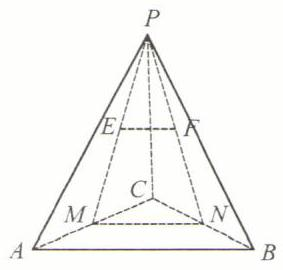
\includegraphics[width=0.2\textwidth]{bodyxb/src/bo_d20cdrf7aajc73bfmvhg_167_452_1692_283_270_0.jpg}
\end{center}


(第 181 题)

\begin{center}
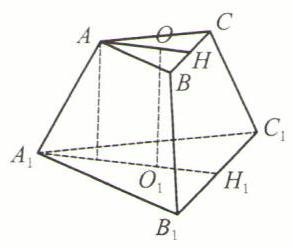
\includegraphics[width=0.2\textwidth]{bodyxb/src/bo_d20cdrf7aajc73bfmvhg_167_818_1712_292_247_0.jpg}
\end{center}


(第 182 题)

182. A 提示: 设上下底面的中心分别为 $O$ 和 ${O}_{1}$ ,棱 ${BC}$ 和 ${B}_{1}{C}_{1}$ 的中点分别为 $H$ 和 ${H}_{1}.{AH} = \sqrt{3},{AO} = \dfrac{2\sqrt{3}}{3}$ ,

${A}_{1}{H}_{1} = 2\sqrt{3},{A}_{1}{O}_{1} = \dfrac{4\sqrt{3}}{3}$ . 又 $\angle A{A}_{1}{H}_{1} = {45}^{ \circ  },\;\therefore \;O{O}_{1} = \left( {\dfrac{4\sqrt{3}}{3} - \dfrac{2\sqrt{3}}{3}}\right)  \cdot  \tan {45}^{ \circ  } = \dfrac{2\sqrt{3}}{3}$ ,

$\therefore V = \dfrac{1}{3} \cdot  \dfrac{2\sqrt{3}}{3} \cdot  \left( {\dfrac{\sqrt{3}}{4} \cdot  {2}^{2} + \dfrac{\sqrt{3}}{4} \cdot  {4}^{2} + \dfrac{\sqrt{3}}{4} \cdot  4 \cdot  2}\right)  = \dfrac{14}{3},\;\therefore$ 选 A.

183. C 提示: $V = \dfrac{1}{3} \cdot  a \cdot  \left( {\dfrac{\sqrt{3}}{4} \cdot  {a}^{2} \cdot  6 + \dfrac{\sqrt{3}}{4} \cdot  4{a}^{2} \cdot  6 + \sqrt{\dfrac{\sqrt{3}}{4} \cdot  {a}^{2} \cdot  6 \cdot  \dfrac{\sqrt{3}}{4} \cdot  4{a}^{2} \cdot  6}}\right)  = \dfrac{1}{3} \cdot  a \cdot$

$\left( {\dfrac{3\sqrt{3}}{2}{a}^{2} + 6\sqrt{3}{a}^{2} + 3\sqrt{3}{a}^{2}}\right)  = \dfrac{7\sqrt{3}}{2}{a}^{3},\;\therefore \;$ 选 C.

184. D 提示: 不妨设棱长为 $1,{V}_{{NM}{G}_{1} - {HFG}} = \dfrac{1}{3} \cdot  1 \cdot  \left( {\dfrac{1}{8} + \dfrac{1}{2} + \sqrt{\dfrac{1}{8} \cdot  \dfrac{1}{2}}}\right)  = \dfrac{7}{24},\therefore \dfrac{{V}_{1}}{{V}_{2}} = \dfrac{1 - \dfrac{7}{24}}{\dfrac{7}{24}} = \dfrac{17}{7},\therefore$ 选 D.

185. A 提示: 如图,设棱台上底面面积为 ${S}_{1}$ ,下底面面积为 ${S}_{2}$ ,棱台高 $h.\dfrac{{S}_{1}}{{S}_{2}} = {\left( \dfrac{1}{2}\right) }^{2}$ ,得 ${S}_{2}$  $= 4{S}_{1}$ .

\begin{center}
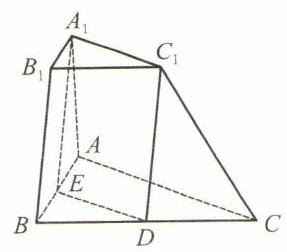
\includegraphics[width=0.2\textwidth]{bodyxb/src/bo_d20cdrf7aajc73bfmvhg_168_1249_516_287_252_0.jpg}
\end{center}


(第 185 题)

${V}_{\text{ 棱台 }} = \dfrac{1}{3}h\left( {{S}_{1} + {S}_{2} + \sqrt{{S}_{1}{S}_{2}}}\right)  = \dfrac{7}{3}h{S}_{1}$ ,而 ${V}_{\text{ 棱柱 }} = {S}_{1} \cdot  h,\;\therefore \;\dfrac{{V}_{\text{ 棱台 }}}{{V}_{\text{ 棱柱 }}} = \dfrac{7}{3}$ ,

$\therefore \dfrac{{V}_{\text{ 棱台 }} - {V}_{\text{ 棱柱 }}}{{V}_{\text{ 棱柱 }}} = \dfrac{7 - 3}{3} = \dfrac{4}{3},\;\therefore \;$ 选 A.

186. B 提示: 设圆台上、下底面半径分别为 $r,{3r}$ ,高为 $h$ . 则 $\left\{  \begin{array}{l} \dfrac{1}{3}{\pi h}\left( {{r}^{2} + 9{r}^{2} + 3{r}^{2}}\right)  = {234}\mathrm{v} \\  {2\pi r} = \pi  \cdot  \sqrt{{r}^{2} + {\left( \dfrac{h}{2}\right) }^{2}}, \end{array}\right.$  $\left\{  {\begin{array}{l} r = 3, \\  h = 6\sqrt{3}, \end{array}{3r} = 9,}\right.$  $\therefore$ 选 B.

187. $B$ 提示:如图,由圆台的轴截面,得圆台的高 $h = \sqrt{{\left( R + r\right) }^{2} - {\left( R - r\right) }^{2}} = 2\sqrt{Rr},\;\therefore V = \dfrac{1}{3}$  $\left( {\pi {r}^{2} + \pi {R}^{2} + {\pi rR}}\right)  \cdot  2\sqrt{Rr} = \dfrac{2\pi }{3}\left( {{r}^{2} + {R}^{2} + {rR}}\right)  \cdot  \sqrt{Rr},\;\therefore$ 选B.

\begin{center}
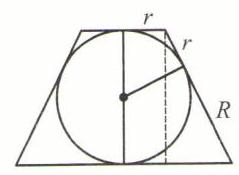
\includegraphics[width=0.2\textwidth]{bodyxb/src/bo_d20cdrf7aajc73bfmvhg_168_1300_1045_239_175_0.jpg}
\end{center}


(第 187 题)

188. (1) ${27}\sqrt{3}\;9\sqrt{3}$ 提示: 侧棱长为 $\sqrt{21}$ ,底面三角形的边长为 $6,{S}_{\text{ 全 }} = \dfrac{\sqrt{3}}{4} \cdot  {6}^{2} + 3$ . $\left( {\dfrac{1}{2} \cdot  6 \cdot  2\sqrt{3}}\right)  = {27}\sqrt{3},V = \dfrac{1}{3} \cdot  \dfrac{\sqrt{3}}{4} \cdot  {6}^{2} \cdot  3 = 9\sqrt{3}.$

(2) 1 提示: $V = \dfrac{1}{2} \cdot  1 \cdot  2 \cdot  3 \cdot  \dfrac{1}{3} = 1{\mathrm{\;{cm}}}^{3}$ .

(3)4 提示:由已知,三条侧棱两两垂直. 设 3 条侧棱分别为 $a,b,c$ 则 $\times  \left\{  \begin{array}{l} \dfrac{1}{2} \cdot  a \cdot  b = 6, \\  \dfrac{1}{2} \cdot  b \cdot  c = 4,\text{ 得 }{\left( abc\right) }^{2} = {576}, \\  \dfrac{1}{2} \cdot  a \cdot  c = 3, \end{array}\right. \;\therefore \;V = \dfrac{1}{6}{abc}$  $= 4$ .

(4) $\dfrac{{a}^{3}}{3} - \dfrac{2\sqrt{3}}{3}a$ 提示: $V = {a}^{3} - 4 \cdot  \dfrac{1}{3} \cdot  \dfrac{1}{2} \cdot  {a}^{3} = \dfrac{1}{3}{a}^{3}$ ,底面面积 $S = \dfrac{\sqrt{3}}{4} \cdot  {\left( \sqrt{2}a\right) }^{2} = \dfrac{\sqrt{3}}{2}{a}^{2},\;\therefore h = \dfrac{3V}{S} = \dfrac{2\sqrt{3}}{3}a$ . (5) $\dfrac{24}{5}$ 提示: $h = \dfrac{3 \times  4}{5} = \dfrac{12}{5}\mathrm{\;{cm}},V = \left( {\dfrac{1}{2} \cdot  3 \cdot  4}\right)  \cdot  \dfrac{12}{5} \cdot  \dfrac{1}{3} = \dfrac{24}{5}{\mathrm{\;{cm}}}^{3}$ .

(6) $\dfrac{1}{6}\sqrt{{S}^{2}Q - {Q}^{3}}$ 提示:如图, ${h}_{\text{ 侧 }} = \dfrac{2S}{\sqrt{Q}} \cdot  \dfrac{1}{4} = \dfrac{S}{2\sqrt{Q}},h = \sqrt{{h}_{\text{ 侧 }}^{2} - {\left( \dfrac{\sqrt{Q}}{2}\right) }^{2}} = \dfrac{1}{2} \cdot  \sqrt{\dfrac{{S}^{2} - {Q}^{2}}{Q}}$ ,

\begin{center}
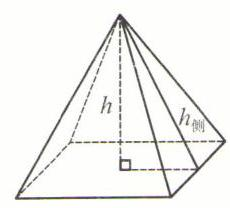
\includegraphics[width=0.2\textwidth]{bodyxb/src/bo_d20cdrf7aajc73bfmvhg_168_1310_1816_230_208_0.jpg}
\end{center}


[第 188(6)题]

$\therefore V = \dfrac{1}{3} \cdot  S \cdot  h = \dfrac{1}{3} \cdot  Q \cdot  \dfrac{1}{2} \cdot  \sqrt{\dfrac{{S}^{2} - {Q}^{2}}{Q}} = \dfrac{1}{6}\sqrt{{S}^{2}Q - {Q}^{3}}$ .

(7) $\dfrac{1}{2}V$ 提示: $\dfrac{{V}_{\text{ 角 }}}{{V}_{\text{ 原 }}} = {\left( \dfrac{1}{2}\right) }^{3} = \dfrac{1}{8},\;\therefore \;{V}_{\text{ 斜 }} = {V}_{\text{ 原 }} - 4{V}_{\text{ 角 }} = V - 4 \cdot  \dfrac{1}{8}V = \dfrac{1}{2}V$ .

189. (1) 2 倍 提示: $\dfrac{{V}_{\text{ 新 }}}{{V}_{\text{ 原 }}} = \dfrac{\dfrac{1}{3} \cdot  {S}_{\text{ 新 }} \cdot  {h}_{\text{ 新 }}}{\dfrac{1}{3} \cdot  {Sh}} = \dfrac{\dfrac{1}{3} \cdot  \pi {\left( 2r\right) }^{2} \cdot  \dfrac{1}{2}h}{\dfrac{1}{3} \cdot  \pi {r}^{2} \cdot  h} = 2$ .

(2) $9\sqrt{15}\pi$ 提示: ${2\pi r} = \dfrac{1}{4} \cdot  {2\pi } \cdot  {12}$ 得 $r = 3\mathrm{\;{cm}},\;\therefore h = \sqrt{{12}^{2} - {r}^{2}} = 3\sqrt{15}\mathrm{\;{cm}}$ ,

$\therefore \;V = \dfrac{1}{3} \cdot  \pi {r}^{2} \cdot  h = 9\sqrt{15}\pi {\mathrm{\;{cm}}}^{3}.$

(3) $\dfrac{3V}{\pi S}$ 提示: $\left\{  \begin{array}{l} {rh} = S, \\  \dfrac{1}{3}\pi {r}^{2} \cdot  h = V, \end{array}\right.$ 得 $r = \dfrac{3V}{\pi S}$ .

(4) $\dfrac{\pi }{4}{a}^{3}$ 提示: $V = 2 \cdot  \dfrac{1}{3} \cdot  \pi {\left( \dfrac{\sqrt{3}a}{2}\right) }^{2} \cdot  \dfrac{a}{2} = \dfrac{\pi }{4}{a}^{3}$ .

190. (1) ${3020\pi }$ 提示: 设圆台高为 $h\mathrm{\;{cm}}$ ,则 $\dfrac{1}{2} \cdot  \left( {{10} + {18}}\right)  \cdot  2 \cdot  h = {420}$ ,解得 $h = {15}\mathrm{\;{cm}}$ .

$\therefore V = \dfrac{1}{3} \cdot  \left( {{10}^{2} + {18}^{2} + \sqrt{{10}^{2} \cdot  {18}^{2}}}\right)  \cdot  \pi  \cdot  {15} = {3020\pi }{\mathrm{\;{cm}}}^{3}$ .

(2)8 提示:设另一个底面面积为 $S$ ,则 ${76} = \dfrac{1}{3} \cdot  6 \cdot  \left( {{18} + S + \sqrt{{18} \cdot  S}}\right)$ ,解得 $S = 8{\mathrm{\;{cm}}}^{2}$ .

(3) $\dfrac{{28}\sqrt{2}}{3}$ 提示:由经过棱台一组相对侧棱的平面,得棱台的高. 如图, $h = \left( {2\sqrt{2} - \sqrt{2}}\right)  \cdot  \tan {45}^{ \circ  } = \sqrt{2},\therefore V = \dfrac{1}{3}$ . $\sqrt{2} \cdot  \left( {{2}^{2} + {4}^{2} + \sqrt{{2}^{2} \cdot  {4}^{2}}}\right)  = \dfrac{{28}\sqrt{2}}{3}{\mathrm{\;{cm}}}^{3}.$

\begin{center}
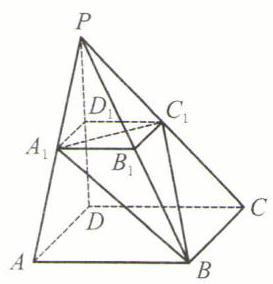
\includegraphics[width=0.2\textwidth]{bodyxb/src/bo_d20cdrf7aajc73bfmvhg_169_844_972_273_284_0.jpg}
\end{center}


[第 190(5)题]

\begin{center}
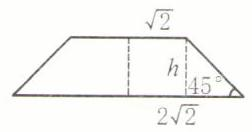
\includegraphics[width=0.2\textwidth]{bodyxb/src/bo_d20cdrf7aajc73bfmvhg_169_483_1123_252_132_0.jpg}
\end{center}


[第 190(3)题]

(4)50 128 提示:设上、下底面面积分别为 ${25x}$ , ${64x}$ . 则 ${1720} = \dfrac{1}{3} \cdot  {20} \cdot  \left( {{25x} + {64x} + \sqrt{{25x} \cdot  {64x}}}\right)$ ,解得 $x = 2$ ,

$\therefore {25x} = {50},{64x} = {128}$ ,即上、下底面的面积分别为 50,128 .

(5) $\dfrac{V}{14}$ 提示:如图,将四棱台补成以 $P$ 为顶点的四棱锥. ∵ ${A}_{1}{B}_{1} = a,{AB} = {2a},\therefore \dfrac{{V}_{P - {A}_{1}{B}_{1}{C}_{1}{D}_{1}}}{{V}_{P - {ABCD}}} = {\left( \dfrac{a}{2a}\right) }^{3} = \dfrac{1}{8}$

$\Rightarrow  \dfrac{{V}_{P - {A}_{1}{B}_{1}{C}_{1}{D}_{1}}}{{V}_{{A}_{1}{B}_{1}{C}_{1}{D}_{1} - {ABCD}}} = \dfrac{1}{7}.$

又 ${V}_{{A}_{1}{B}_{1}{C}_{1}{D}_{1} - {ABCD}} = V,\therefore {V}_{P - {A}_{1}{B}_{1}{C}_{1}{D}_{1}} = \dfrac{V}{7}$ . 又 $\dfrac{{h}_{P - {A}_{1}{B}_{1}{C}_{1}{D}_{1}}}{{h}_{P - {ABCD}}} = \dfrac{a}{2a} = \dfrac{1}{2}$ ,

$\therefore {V}_{B - {A}_{1}{B}_{1}{C}_{1}} = {V}_{P - {A}_{1}{B}_{1}{C}_{1}} = \dfrac{1}{2}{V}_{P - {A}_{1}{B}_{1}{C}_{1}{D}_{1}} = \dfrac{1}{2} \cdot  \dfrac{V}{7} = \dfrac{V}{14}$ .

191. (1) 由题意,底面半径 $r = 4\mathrm{\;{cm}}$ ,则高 $h = 4 \cdot  \cot {30}^{ \circ  } = 4\sqrt{3}\mathrm{\;{cm}},\therefore V = \dfrac{1}{3}\pi {r}^{2} \cdot  h = \dfrac{{64}\sqrt{3}}{3}\pi {\mathrm{{cm}}}^{3}$ .

(2)如图,设圆锥体积为 $V$ ,则水的体积为 $\dfrac{V}{8}$ . 倒转后, ${\left( \dfrac{{h}_{1}}{2h}\right) }^{3} = \dfrac{7}{8} \Rightarrow  {h}_{1} = \sqrt[3]{7}h$ , 则 ${h}_{ \star  } = {2h} - \sqrt[3]{7}h = \left( {2 - \sqrt[3]{7}}\right) h$ .

\begin{center}
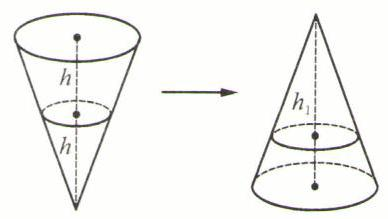
\includegraphics[width=0.3\textwidth]{bodyxb/src/bo_d20cdrf7aajc73bfmvhg_169_1057_1824_388_219_0.jpg}
\end{center}


[第 191(2)题]

192. (1) 如图,作 ${EM} \bot  {AF}$ ,在 Rt $\bigtriangleup {AEF}$ 中, ${AE} = \dfrac{a}{2},{AF} = \dfrac{\sqrt{3}}{2}a \Rightarrow  {EF} =$  $\sqrt{A{F}^{2} - A{E}^{2}} = \dfrac{\sqrt{2}}{2}a,r = {EM} = \dfrac{{AE} \cdot  {EF}}{AF} = \dfrac{\sqrt{6}}{6}a,$

$\therefore V = \dfrac{1}{3} \cdot  \pi  \cdot  {r}^{2} \cdot  {AF} = \dfrac{1}{3} \cdot  \pi  \cdot  {\left( \dfrac{\sqrt{6}}{0}a\right) }^{2} \cdot  \dfrac{\sqrt{3}}{3}a = \dfrac{\sqrt{3}\pi }{36}{a}^{3}$ .

\begin{center}
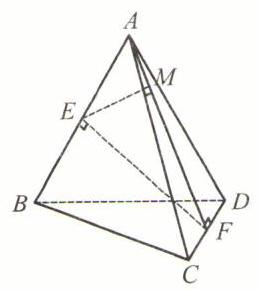
\includegraphics[width=0.2\textwidth]{bodyxb/src/bo_d20cdrf7aajc73bfmvhg_170_553_142_258_290_0.jpg}
\end{center}


[第 192(1)题]

\begin{center}
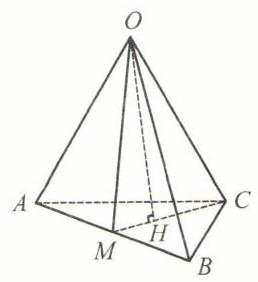
\includegraphics[width=0.2\textwidth]{bodyxb/src/bo_d20cdrf7aajc73bfmvhg_170_917_146_258_282_0.jpg}
\end{center}


[第 192(2)题]

(2)如图,作 ${OH} \bot$ 平面 ${ABC}$ 于点 $H$ ,设 ${CH} = a$ ,则 ${OC} = {3a}$ , $\therefore {OH} = 2\sqrt{2}a$ . 又 ${MH} = \left| {\dfrac{\sqrt{3}}{2} - a}\right| ,{OM} = \dfrac{\sqrt{3}}{2}$ ,在 Rt

$\bigtriangleup {OMH}$ 中, ${\left( \dfrac{\sqrt{3}}{2} - a\right) }^{2} + {\left( 2\sqrt{2}a\right) }^{2} = {\left( \dfrac{\sqrt{3}}{2}\right) }^{2}$ ,解得 $a = \dfrac{\sqrt{3}}{9},\;\therefore \;V = \dfrac{1}{3} \cdot  \dfrac{\sqrt{3}}{4} \cdot  \left( {2\sqrt{2} \cdot  \dfrac{\sqrt{3}}{9}}\right)  = \dfrac{\sqrt{2}}{18}$ .

(3)由例 8 的结论, ${V}_{P - {ABC}} = \dfrac{1}{6} \cdot  {a}^{2} \cdot  h = \dfrac{{a}^{2}h}{6}$ .

193. (1) ${V}_{A - {BQC}} = {V}_{Q - {ABC}} = \dfrac{1}{3} \cdot  {S}_{\bigtriangleup {ABC}} \cdot  {h}_{Q} = \dfrac{1}{3} \cdot  \left( {\dfrac{1}{2} \cdot  4}\right)  \cdot  {h}_{Q}$ .

当 ${h}_{Q\max } = 1$ 时, ${V}_{A - {BQC}\max } = \dfrac{2}{3}$ ,此时 ${V}_{A - {BQC}} = \dfrac{1}{3} \cdot  {S}_{\bigtriangleup {ABQ}} \cdot  {h}_{C}$ ,即 $\dfrac{2}{3} = \dfrac{1}{3}\left( {\dfrac{1}{2} \cdot  \sqrt{2} \cdot  2}\right)  \cdot  {h}_{C}$ ,即 ${h}_{C} = \sqrt{2}$ .

(2)设圆锥的母线长为 $l$ ,高为 $h$ ,底面半径为 $r$ ,则 $\pi  = \pi {r}^{2} + {\pi rl}$ , $\therefore l = \dfrac{1 - {r}^{2}}{r},h = \sqrt{{l}^{2} - {r}^{2}} = \dfrac{\sqrt{1 - 2{r}^{2}}}{r}$ ,

$\therefore {V}_{\text{ 圆锥 }} = \dfrac{1}{3}\pi {r}^{2} \cdot  h = \dfrac{{\pi r} \cdot  \sqrt{1 - 2{r}^{2}}}{3} = \dfrac{\pi }{3} \cdot  \sqrt{{r}^{2} - 2{r}^{4}} = \dfrac{\pi }{3}\sqrt{-2{\left( {r}^{2} - \dfrac{1}{4}\right) }^{2} + \dfrac{1}{8}}$ ,

$\therefore$ 当 $r = \dfrac{1}{2}$ 时, ${V}_{\max } = \dfrac{\sqrt{2}\pi }{12}$ .

194. B 提示: $\dfrac{{V}_{1}}{{V}_{2}} = \dfrac{\pi {b}^{2} \cdot  a}{\pi {a}^{2} \cdot  b} = \dfrac{b}{a},\;\therefore \;$ 选B.

195. B 提示: 设小圆锥和原圆锥的面积分别为 ${S}_{1}$ 和 $S$ ,体积分别为 ${V}_{1}$ 和 $V.\dfrac{{S}_{1}}{S} = \dfrac{1}{2}$ ,则 $\dfrac{{h}_{1}}{h} = \sqrt{\dfrac{1}{2}}$ ,则 $\dfrac{{V}_{1}}{V} = {\left( \sqrt{\dfrac{1}{2}}\right) }^{3} =$  ${2}^{-\dfrac{3}{2}}$ . 又 ${V}_{1} = 1,\;\therefore \;V = {2}^{\dfrac{3}{2}} = 2\sqrt{2},\;\therefore \;$ 选 B.

196. $C$ 提示: $\dfrac{1}{3} \times  {30} = {10},\therefore$ 选 $C$ .

197. D 提示:如图, ${V}_{A - {GEF}} = \dfrac{1}{2}{V}_{E - {AFD}} = \dfrac{1}{2} \cdot  \dfrac{1}{2}{V}_{{A}_{1} - {AFD}} = \dfrac{1}{2} \cdot  \dfrac{1}{2} \cdot  \dfrac{1}{2}{V}_{{A}_{1} - {ABD}} = \dfrac{1}{2} \cdot  \dfrac{1}{2} \cdot  \dfrac{1}{2}$ . $\dfrac{1}{2}{V}_{{A}_{1} - {ABCD}} = \dfrac{1}{2} \cdot  \dfrac{1}{2} \cdot  \dfrac{1}{2} \cdot  \dfrac{1}{2} \cdot  \dfrac{1}{3} \cdot  {V}_{{ABCD} - {A}_{1}{B}_{1}{C}_{1}{D}_{1}} = \dfrac{1}{48}{V}_{{ABCD} - {A}_{1}{B}_{1}{C}_{1}{D}_{1}},\;\therefore \;$ 选 D.

\begin{center}
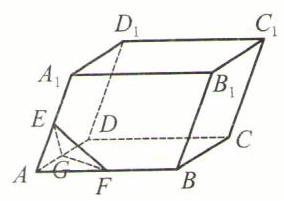
\includegraphics[width=0.2\textwidth]{bodyxb/src/bo_d20cdrf7aajc73bfmvhg_170_1242_1381_284_201_0.jpg}
\end{center}


(第 197 题)

198. $C$ 提示: $\dfrac{\dfrac{1}{2} \times  \dfrac{1}{3} \times  \dfrac{3}{4}}{1 \times  1 \times  1} = \dfrac{1}{{V}_{P - {ABC}}},\therefore {V}_{P - {ABC}} = 8$ ,则 ${V}_{{EFG} - {ABC}} = 8 - 1 = 7,\therefore$ 选 $C$ .

199. C 提示: 三个旋转体的体积比为 $\dfrac{\pi }{3}{\left( b\sin C\right) }^{2}a : \dfrac{\pi }{3}{\left( c\sin A\right) }^{2}b : \dfrac{\pi }{3}{\left( a\sin B\right) }^{2}c = {b}^{2}{c}^{2}a$ : ${c}^{2}{a}^{2}b : {a}^{2}{b}^{2}c = \dfrac{1}{a} : \dfrac{1}{b} : \dfrac{1}{c},\therefore$ 选 C.

200. D 提示: 设它到四个面的距离分别为 $a,b,c,d$ . 一个面的面积为 $S = \dfrac{1}{2} \cdot  1 \cdot  1 \cdot  \sin {60}^{ \circ  } = \dfrac{\sqrt{3}}{4}$ ,

顶点在底面的投影是底面中心,到底面三个顶点的距离都是高的 $\dfrac{2}{3}$ ,高为 $1 \cdot  \sin {60}^{ \circ  } = \dfrac{\sqrt{3}}{2}$ ,

$\therefore$ 底面中心到底面顶点的距离为 $\dfrac{\sqrt{3}}{3},\therefore$ 顶点到底面的距离为 $\sqrt{{1}^{2} - {\left( \dfrac{\sqrt{3}}{3}\right) }^{2}} = \dfrac{\sqrt{6}}{3}$ .

$\therefore V = \dfrac{1}{3} \cdot  \dfrac{\sqrt{3}}{4} \cdot  \dfrac{\sqrt{6}}{3} = \dfrac{\sqrt{2}}{12}$ ,又 $\dfrac{1}{3} \cdot  \dfrac{\sqrt{3}}{4} \cdot  \left( {a + b + c + d}\right)  = V,\;\therefore a + b + c + d = \dfrac{\sqrt{6}}{3}.\;\therefore$ 选 D.

201. D 提示: 设三部分的体积依次为 ${V}_{1},{V}_{2},{V}_{3}$ ,则 ${V}_{1} : \left( {{V}_{1} + {V}_{2}}\right)  : \left( {{V}_{1} + {V}_{2} + {V}_{3}}\right)  = {1}^{3} : {2}^{3} : {3}^{3}$ ,

$\therefore {V}_{1} : {V}_{2} : {V}_{3} = 1 : 7 : {19},\therefore$ 选 D.

202. (1) $\dfrac{15}{2}$ 提示: ${V}_{P - {ABC}} = \dfrac{1}{3}{S}_{\bigtriangleup {APB}} \cdot  {PC} = \dfrac{1}{3} \cdot  \dfrac{1}{2} \cdot  5 \cdot  4 \cdot  3 = {10}$ ,

又 ${V}_{P - {ABC}} = \dfrac{1}{3}{S}_{\bigtriangleup {ABC}} \cdot  h = {10},\therefore {S}_{\bigtriangleup {ABC}} \cdot  h = {30}$ .

又 $\dfrac{{S}_{\bigtriangleup {ADE}}}{{S}_{\bigtriangleup {ABC}}} = \dfrac{1}{4},\therefore \dfrac{{S}_{\text{ 四边形 }{BCED}}}{{S}_{\bigtriangleup {ABC}}} = \dfrac{3}{4}$ .

$\therefore {V}_{P - {BCED}} = \dfrac{1}{3}{S}_{\text{ 四边形 BCED }} \cdot  h = \dfrac{1}{3} \cdot  \dfrac{3}{4} \cdot  {S}_{\bigtriangleup {ABC}} \cdot  h = \dfrac{1}{3} \cdot  \dfrac{3}{4} \cdot  {30} = \dfrac{15}{2}$ .

(2) $\dfrac{\sqrt{6}a}{2}\;\dfrac{{a}^{3}}{8}$ 提示: 设 ${PA} = x\mathrm{\;{cm}}$ ,则 ${V}_{P \cdot  {ABC}} = 2 \cdot  \dfrac{1}{3} \cdot  \left( {\sqrt{\dfrac{3{a}^{2}}{4} - \dfrac{{x}^{2}}{4}} \cdot  a \cdot  \dfrac{1}{2}}\right)  \cdot  \dfrac{x}{2} = \dfrac{ax}{12}\sqrt{3{a}^{2} - {x}^{2}} = \dfrac{a}{12}$ .

$\sqrt{-{\left( {x}^{2} - \dfrac{3}{2}{a}^{2}\right) }^{2} + \dfrac{9}{4}{a}^{4}},x \in  \left( {0,\sqrt{3}a}\right) ,\;\therefore \;x = \dfrac{\sqrt{6}}{2}a$ 时, ${V}_{P - {ABC}\max } = \dfrac{{a}^{3}}{8}$ .

203. (1)取 ${A}_{1}{B}_{1}$ 中点 $G$ ,棱长为 1. ‘ ${AE}//{C}_{1}G$ , $\therefore {S}_{\bigtriangleup {AE}{C}_{1}} = {S}_{\bigtriangleup {ABG}} = \dfrac{1}{2}{S}_{▱{AE}{C}_{1}G}$ . 又 $\because A{C}_{1} = \sqrt{3},{GE} = \sqrt{2}$ ,

$\therefore {S}_{\bigtriangleup {AE}{C}_{1}} = \dfrac{1}{2} \cdot  \sqrt{3} \cdot  \sqrt{2} \cdot  \dfrac{1}{2} = \dfrac{\sqrt{6}}{4},{V}_{A - E{C}_{1}{D}_{1}} = {S}_{\bigtriangleup {C}_{1}{D}_{1}E} \cdot  {AD} \cdot  \dfrac{1}{3} = \dfrac{1}{6}$ .

又 ${V}_{{D}_{1} - {AE}{C}_{1}} = {S}_{\bigtriangleup {AE}{C}_{1}} \cdot  h \cdot  \dfrac{1}{3} = \dfrac{\sqrt{6}}{12} \cdot  h$ 且 ${V}_{A - E{C}_{1}{D}_{1}} = {V}_{{D}_{1} - {AEG}},\;\therefore h = \dfrac{\sqrt{6}}{3}$ .

(2) ${V}_{{A}_{1} - {C}_{1}{EF}} = \dfrac{1}{3} \cdot  {S}_{\bigtriangleup {C}_{1}{EF}} \cdot  {A}_{1}{D}_{1} = \dfrac{1}{3} \cdot  \dfrac{3}{8} \cdot  1 = \dfrac{1}{8}$ ,

${V}_{E - {A}_{1}{C}_{1}F} = \dfrac{1}{3} \cdot  {S}_{\bigtriangleup {A}_{1}{C}_{1}F} \cdot  h = \dfrac{1}{3} \cdot  \dfrac{\sqrt{6}}{4} \cdot  h = \dfrac{\sqrt{6}}{12}h,$

又 ${V}_{{A}_{1} - {C}_{1}{EF}} = {V}_{E - {A}_{1}{C}_{1}F},\;\therefore \;h = \dfrac{\sqrt{6}}{4}$ .

204. (1) 如图,在平面 $\alpha$ 内作 ${BE}//{AC},{BE} = {AC}$ ,连接 ${DE},{CE}$ . : 四边形 ${ACEB}$ 是平形四边形.

\begin{center}
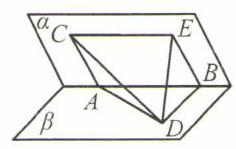
\includegraphics[width=0.2\textwidth]{bodyxb/src/bo_d20cdrf7aajc73bfmvhg_171_1190_1038_236_149_0.jpg}
\end{center}


(第 204 题)

$\because {AC} \bot  {AB},\therefore {AB} \bot  {BE}.\because {AB} \bot  {BD}$ ,

$\therefore \angle {DBE}$ 即二面角平面角,且 ${AB} \bot$ 平面 ${BDE}$ . 又 ${CE}//{AB},\therefore {CE} \bot$ 平面 ${BDE}$ ,

$\therefore \bigtriangleup {CDE}$ 为 $\mathrm{{Rt}}\bigtriangleup$ . 又 ${AB} = 4\mathrm{\;{cm}},{AC} = 6\mathrm{\;{cm}},{BD} = 8\mathrm{\;{cm}},{CD} = 2\sqrt{17}\mathrm{\;{cm}}$ ,则 ${DE} = 2\sqrt{13}$ cm. 由余弦定理得 $\cos \angle {DBE} = \dfrac{B{E}^{2} + B{D}^{2} - D{E}^{2}}{2 \cdot  {BE} \cdot  {BD}} = \dfrac{1}{2}$ ,

$\therefore \angle {DBE} = {60}^{ \circ  }$ ,即二面角 $= {60}^{ \circ  }$ .

(2) $\because {V}_{C - {ABD}} = {V}_{B - {ACD}},\;\therefore \;d = \dfrac{{S}_{\bigtriangleup {ABD}} \cdot  {BE} \cdot  \sin {60}^{ \circ  }}{{S}_{\bigtriangleup {ACD}}} = 2\sqrt{3}\mathrm{\;{cm}}$ .

205. (1) $\because {PA}\bot$ 平面 ${ABC}$ , $\therefore {PA}\bot {BC}$ . 又 $\because {BC}\bot {AC}$ , $\therefore {BC}\bot$ 平面 ${PAC}$ . $\because {AE}$ 在平面 ${PAC}$ 上,

$\therefore {AE} \bot  {BC},{PB} \bot$ 平面 ${ADE},\therefore {AE} \bot  {PB}$ .

又 ${PB} \cap  {BC} = B,\therefore {AE} \bot$ 平面 ${PBC},\therefore {AE} \bot  {DE}$ .

(2)由已知, ${AB} = \sqrt{2}a,{PB} = \sqrt{3}a,{AD} = \dfrac{\sqrt{6}}{3}a,{AE} = \dfrac{\sqrt{2}}{2}a,{DE} = \dfrac{\sqrt{6}}{6}a,{PD} = \dfrac{\sqrt{3}}{3}a$ ,

$\therefore \;{V}_{P - {ADE}} = \dfrac{1}{3} \cdot  \dfrac{1}{2} \cdot  \dfrac{\sqrt{2}}{2}a \cdot  \dfrac{\sqrt{6}}{6}a \cdot  \dfrac{\sqrt{3}}{3}a = \dfrac{{a}^{3}}{36}$ .

206. ${AB} = {AD},{BC} = {DC},{AC} = {AC},\therefore \bigtriangleup {ABC} \cong  \bigtriangleup {ADC}$ .

又 $\angle {BAD} = {120}^{ \circ  },\angle {BCD} = {60}^{ \circ  },\therefore \angle {ABC} = \angle {ADC} = {90}^{ \circ  }$ ,

即 ${AM} \bot  {ME}$ 且 ${AM} \bot  {MF},\;\therefore \;{AM} \bot$ 平面 ${MEF}$ ,

${V}_{A - {MEF}} = \dfrac{1}{3} \cdot  {AM} \cdot  {S}_{\bigtriangleup {MEF}} = \dfrac{1}{3} \cdot  1 \cdot  \left( {\dfrac{1}{2} \cdot  \dfrac{\sqrt{3}}{2} \cdot  \dfrac{\sqrt{3}}{2} \cdot  \sin {60}^{ \circ  }}\right)  = \dfrac{\sqrt{3}}{16}.$

207. (1)如图, $F$ 为 $A{A}_{1}$ 的三等分点, $E$ 为 $B{B}_{1}$ 的三等分点. ${A}_{1}Q//{FC}$ , ${FE}//{AP}$ ,即 $\angle {EFC}$ 为 ${AP}$ 与 ${A}_{1}Q$ 所成角或其补角.

\begin{center}
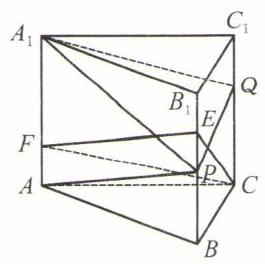
\includegraphics[width=0.2\textwidth]{bodyxb/src/bo_d20cdrf7aajc73bfmvhg_171_1163_1861_265_264_0.jpg}
\end{center}


(第 207 题)

又 ${FE} = {CF} = 3\sqrt{2},{CE} = 3\sqrt{5},\;\therefore \;\cos \angle {EFC} = \dfrac{{\left( 3\sqrt{2}\right) }^{2} + {\left( 3\sqrt{2}\right) }^{2} - {\left( 3\sqrt{5}\right) }^{2}}{2 \cdot  3\sqrt{2} \cdot  3\sqrt{2}} =  - \dfrac{1}{4}$ ,

$\therefore {AP}$ 与 ${A}_{1}Q$ 所成角的余弦值为 $\dfrac{1}{4}$ .

2) ${V}_{\Lambda  \sim  {DO}{\Lambda }_{1}} = {V}_{\Lambda {M}^{\prime } \sim  {\Lambda }_{1}{R}_{1}{\Gamma }_{1}} - {V}_{\Lambda  \sim  {MTOP}} - {V}_{{\Lambda }_{1} \sim  {R}_{1}{\Gamma }_{1}{OP}} = \left( {\dfrac{\sqrt{3}}{4} \cdot  {3}^{2}}\right)  \cdot  9 - \dfrac{1}{3} \cdot  {S}_{\text{ 四边形 }R{C}_{1}{R}_{1}} \cdot  \dfrac{3\sqrt{3}}{2} =$

$\dfrac{81}{4}\sqrt{3} - \dfrac{1}{3} \cdot  {27} \cdot  \dfrac{3\sqrt{3}}{2} = \dfrac{27}{4}\sqrt{3}.$

208. (1) $\because$ 点 ${B}_{1}$ 在底面的射影 $D$ 为 ${BC}$ 的中点, $\therefore {B}_{1}D \bot$ 底面 ${ABC}$ .

又 ${AC}$ 在平面 ${ABC}$ 上, $\therefore {B}_{1}D \bot  {AC}.\because \angle {ACB} = {90}^{ \circ  },\therefore {AC} \bot  {BC}$ .

又 ${BC} \cap  {B}_{1}D = D,\therefore {AC} \bot$ 平面 ${BC}{C}_{1}{B}_{1},\therefore$ 平面 ${BC}{C}_{1}{B}_{1} \bot$ 平面 ${ABC}$ .

由 ${B}_{1}D \bot  {BC}$ 且 $D$ 是 ${BC}$ 中点, $\therefore \bigtriangleup {B}_{1}{BC}$ 为等腰三角形, ${B}_{1}B = {B}_{1}C$ .

又 $\angle {B}_{1}{BC} = {60}^{ \circ  },\therefore \bigtriangleup {B}_{1}{BC}$ 为等边三角形, $\therefore$ 四边形 $B{B}_{1}{C}_{1}C$ 为菱形.

$\therefore {B}_{1}C \bot  B{C}_{1}$ . 又 ${AC} \bot$ 平面 $B{B}_{1}{C}_{1}C,\therefore$ 由三垂线定理 $A{B}_{1} \bot  B{C}_{1}$ .

( 2 )取 $B{B}_{1}$ 中点 $M$ ,连接 ${AM}$ , ${CM}$ , ${AD}$ . 在 $\mathrm{{Rt}} \bigtriangleup  {ACB}$ 中, $A{B}^{2} = B{C}^{2} + A{C}^{2}$ .

在 $\mathrm{{Rt}} \bigtriangleup  {ADB}_{1}$ 中, ${AB}_{1}^{2} = {AD}^{2} + {B}_{1}{D}^{2} = {AC}^{2} + {CD}^{2} + {B}_{1}{D}^{2} = {AC}^{2} + {B}_{1}{C}^{2}$ .

又 $\because {B}_{1}C = {BC},\therefore {AB} = A{B}_{1},\therefore {AM} \bot  B{B}_{1}$ .

又 $\bigtriangleup {BC}{B}_{1}$ 为正三角形, $\therefore {CM} \bot  B{B}_{1}$ .

$\therefore \angle {AMC}$ 即二面角的平面角, $\therefore \angle {AMC} = {30}^{ \circ  }$

$\therefore$ 在 Rt $\bigtriangleup {ACM}$ 中, ${MC} = \sqrt{3}\mathrm{\;{cm}},{AC} = 1\mathrm{\;{cm}}$ .

$\therefore \;{V}_{A - {B}_{1}{BC}{C}_{1}} = \dfrac{1}{3} \cdot  {S}_{{BC}{C}_{1}{B}_{1}} \cdot  {AC} = \dfrac{2}{3}\sqrt{3}{\mathrm{\;{cm}}}^{3}$ .

209. (1) 如图, $A{A}_{1} = h,{A}_{1}B = {2R} \cdot  \sin \dfrac{\theta }{2}$ 或 ${2R}\cos \dfrac{\theta }{2}$ . 在 $\mathrm{{Rt}} \bigtriangleup  A{A}_{1}B$ 中, $\tan \angle {BA}{A}_{1} = \dfrac{{A}_{1}B}{A{A}_{1}} =$  $\dfrac{2R}{h}\sin \dfrac{\theta }{2}$ 或 $\dfrac{2R}{h}\cos \dfrac{\theta }{2}$ ,即 $O{O}_{1}$ 与 ${AB}$ 所成角的正切值为 $\dfrac{2R}{h}\sin \dfrac{\theta }{2}$ 或 $\dfrac{2R}{h}\cos \dfrac{\theta }{2}$ . (2) $V = {V}_{B - {O}_{1}A} = \dfrac{1}{3} \cdot  {S}_{\bigtriangleup {O}_{1}A} \cdot  {O}_{1}B \cdot  \sin \theta  = \dfrac{1}{6}{R}^{2}h\sin \theta$ . 210. (1) $\because$ 平面 ${BC}{C}^{\prime }{B}^{\prime } \bot$ 底面 ${ABC},\therefore \angle {C}^{\prime }{CB}$ 即侧棱 ${C}^{\prime }C$ 与底面所成角, 即 $\angle {C}^{\prime }{CB} = {60}^{ \circ  }$ ,又 ${C}^{\prime }C = {CB} = a,\therefore \bigtriangleup {C}^{\prime }{CB}$ 为等边三角形. 取 ${BC}$ 中点 $H$ ,连接 ${C}^{\prime }H,{AH}$ ,则 ${C}^{\prime }H \bot  {BC}$ . 又 ${AC} = {AB},\therefore {AH}\bot {BC},\therefore {BC}\bot$ 平面 ${C}^{\prime }{HA},\therefore {C}^{\prime }A\bot {BC}$ .

\begin{center}
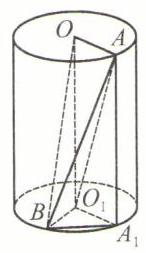
\includegraphics[width=0.2\textwidth]{bodyxb/src/bo_d20cdrf7aajc73bfmvhg_172_1324_775_146_253_0.jpg}
\end{center}


(第 209 题)

(2) ${V}_{\text{ 柱 }} = {S}_{\bigtriangleup {ABC}} \cdot  h = \dfrac{\sqrt{3}}{4}{a}^{2} \cdot  \dfrac{\sqrt{3}}{2}a = \dfrac{3}{8}{a}^{3},\;\therefore \;{V}_{{C}^{\prime } - {AB}{B}^{\prime }{A}^{\prime }} = {V}_{\text{ 柱 }} - {V}_{{C}^{\prime } - {ABC}} = \left( {1 - \dfrac{1}{3}}\right)  \cdot  {V}_{\text{ 柱 }} = \dfrac{1}{4}{a}^{3}$ .

211. (1) ${V}_{B - {AEF}} = {V}_{{D}_{1} - {AEF}}$ . 又 ${V}_{B - {AEF}} = \dfrac{1}{3} \cdot  {S}_{\bigtriangleup {AEF}} \cdot  {h}_{B} = \dfrac{1}{3} \cdot  \dfrac{\sqrt{2}}{4}{a}^{2} \cdot  \dfrac{\sqrt{2}}{2}a = \dfrac{{a}^{3}}{12}$ ,

$\therefore \;{V}_{{A}_{1} - {EBF}{D}_{1}} = 2{V}_{B - {AEF}} = \dfrac{{a}^{3}}{6}$ .

2) ${V}_{B - {APQC}} = \dfrac{1}{2}{V}_{B - {A}^{\prime }{AC}{C}^{\prime }} = \dfrac{1}{2} \cdot  \left( {{V}_{{ABC} - {A}^{\prime }{B}^{\prime }{C}^{\prime }} - {V}_{B - {A}^{\prime }{B}^{\prime }{C}^{\prime }}}\right)  = \dfrac{1}{2} \cdot  \dfrac{2}{3} \cdot  V = \dfrac{V}{3}$ .

(3)过点 ${B}_{1}$ 作 ${B}_{1}K//{FA}$ 交 ${CB}$ 延长线于点 $K$ ,则 ${V}_{{B}_{1} - {AEF}} = {V}_{K - {AEF}} = {V}_{F - {AKE}} = \dfrac{1}{3}{FD} \cdot  {S}_{\bigtriangleup {AKE}}$ .

$\because \;{KE} = \dfrac{5}{2},{S}_{\bigtriangleup {AKE}} = \dfrac{5}{4},\;\therefore \;V = \dfrac{5}{24}$ .

212. $\because {EF}$ 为定长 $b,{C}_{1}{D}_{1}//{AB},\therefore$ 点 $Q$ 到 ${EF}$ 距离为定长 $\sqrt{2}a$ ,

$\therefore {S}_{\bigtriangleup {EFQ}} = \dfrac{1}{2} \cdot  b \cdot  \sqrt{2}a = \dfrac{\sqrt{2}}{2}{ab}$ 为定值.

又点 $P$ 到平面 ${QEF}$ 的距离即到平面 ${AB}{C}_{1}{D}_{1}$ 的距离,当点 $P$ 在点 ${A}_{1}$ 时,距离最大为 $\dfrac{\sqrt{2}}{2}a$ ,

$\therefore \;{V}_{P - {EFQ}\max } = \dfrac{1}{3} \cdot  {S}_{\bigtriangleup {EFQ}} \cdot  {h}_{P\max } = \dfrac{1}{3} \cdot  \dfrac{\sqrt{2}}{2}{ab} \cdot  \dfrac{\sqrt{2}}{2}a = \dfrac{1}{6}{a}^{2}b.$

213. (1)作 ${D}_{1}F \bot  {AE}$ 于点 $F$ , $\because {D}_{1}E = {DE} = 1,A{D}_{1} - {AD} = 1$ 且 ${D}_{1}F \bot  {FE}$ , $\therefore F$ 是 ${AE}$ 中点.

取 ${BC}$ 的中点 $G$ ,连接 ${D}_{1}G,{FG},\because B{D}_{1} = C{D}_{1},\therefore {D}_{1}G \bot  {BC}$ . 又 ${FG} \bot  {BC},\therefore {BC} \bot$ 平面 ${D}_{1}{FG}$ , $\therefore {BC} \bot  {D}_{1}F$ ,则 ${D}_{1}F \bot$ 平面 ${ABC}$ ,平面 $A{D}_{1}E \bot$ 平面 ${ABC}$ .

( 2 )由( 1 )知 $F$ 为点 ${D}_{1}$ 在底面的射影,作 ${D}_{1}H\bot {AB}$ 于点 $H$ ,连接 ${FH}$ . 由三垂线定理 ${FH}\bot {AB}$ ,

$\therefore \angle {D}_{1}{HF}$ 即二面角 ${D}_{1} - {AB} - E$ 的平面角. 在 $\mathrm{{Rt}}\bigtriangleup {D}_{1}{FH}$ 中, $\tan \angle {D}_{1}{HF} = \dfrac{{D}_{1}F}{HF} = \sqrt{2}$ .

(3) ${V}_{{D}_{1} - {ADE}} = \dfrac{1}{3}{S}_{\bigtriangleup {ADD}} \cdot  {D}_{1}F = \dfrac{1}{3} \cdot  2 \cdot  1 \cdot  \dfrac{1}{2} \cdot  \dfrac{\sqrt{2}}{2} = \dfrac{\sqrt{2}}{6}$ . 214. 设正三棱锥底面边长为 $a$ ,高为 $h,{V}_{\text{ 原 }} = \dfrac{\sqrt{3}}{4}{a}^{2} \cdot  h \cdot  \dfrac{1}{3} = \dfrac{\sqrt{3}}{12}{a}^{2}h$ , ${V}_{C - {EFG}} = \dfrac{1}{3}{S}_{\bigtriangleup {EFC}} \cdot  {GD} = \dfrac{1}{3} \cdot  \dfrac{\sqrt{3}}{36}{a}^{2} \cdot  \dfrac{h}{2} = \dfrac{\sqrt{3}{a}^{2}h}{216},\;\therefore \;$ 两部分体积之比为 $1 : {17}$ .

215. (1) 取 ${A}_{1}{B}_{1}$ 中点 ${D}_{1},\because {C}_{1}{D}_{1} \bot$ 平面 ${AB}{B}_{1}{A}_{1},\therefore {C}_{1}{D}_{1} \bot  A{B}_{1}$ .

又 $\because A{B}_{1} \bot  B{C}_{1},\therefore A{B}_{1} \bot  B{D}_{1},\therefore A{B}_{1} \bot  {A}_{1}D$ . ①

又 ${CD}//{C}_{1}{D}_{1},\therefore A{B}_{1} \bot  {CD}$ . ②

由①②, $A{B}_{1}\bot$ 平面 ${A}_{1}{CD}$ .

(2) ${V}_{{A}_{1} - {ACD}} = {V}_{C - {AD}{A}_{1}} = \dfrac{1}{3}{S}_{\bigtriangleup {AD}{A}_{1}} \cdot  {CD} = \dfrac{1}{3} \cdot  5 \cdot  1 = \dfrac{5}{3}$ .

216. D 提示: $6{a}^{2} = 6$ 得棱长 $a = 1\mathrm{\;{cm}}$ . 球半径 $r = \dfrac{a}{2} = \dfrac{1}{2}\mathrm{\;{cm}},\therefore {V}_{\text{ 球 }} = \dfrac{4}{3}\pi {r}^{3} = \dfrac{4}{3}\pi {\left( \dfrac{1}{2}\right) }^{3} = \dfrac{\pi }{6}{\mathrm{\;{cm}}}^{3},\therefore$ 选 D.

217. D 提示: 设圆柱底面半径为 $r$ ,则高为 ${2r}$ ,设球半径 $R$ .

${2\pi r} \cdot  {2r} = {4\pi }{R}^{2}$ ,得 $r = R,\;\therefore \;\dfrac{{V}_{\text{ 柱 }}}{{V}_{\text{ 球 }}} = \dfrac{\pi {r}^{2} \cdot  {2r}}{\dfrac{4}{3}\pi {R}^{3}} = \dfrac{3}{2},\;\therefore \;$ 选 D.

218. D 提示: 设球半径为 $R,\therefore {V}_{\text{ 球 }} = \dfrac{4}{3}\pi {R}^{3}$ . 外切圆柱底面半径为 $R$ ,高为 ${2R}$ ,

$\therefore {V}_{\text{ 柱 }} = \pi {R}^{2} \cdot  {2R} = {2\pi }{R}^{3}$ . 外切等边圆锥高为 ${3R}$ ,底面半径为 $\sqrt{3}R,\therefore {V}_{\text{ 锥 }} = \dfrac{1}{3} \cdot  \pi {\left( \sqrt{3}R\right) }^{2} \cdot  {3R} = {3\pi }{R}^{3}$ .

$\therefore {V}_{\text{ 球 }} : {V}_{\text{ 柱 }} : {V}_{\text{ 锥 }} = 4 : 6 : 9,\therefore$ 选 D.

219. A 提示: 设球半径为 $R$ ,则直径为 ${2R},{V}_{\text{ 球 }} = \dfrac{4}{3}\pi {R}^{3}$ ,

则圆柱底面半径为 $R$ ,高为 ${2R},{V}_{\text{ 柱 }} = \pi {R}^{2} \cdot  {2R} = {2\pi }{R}^{3}$ ,

则圆锥底面半径为 $R$ ,高为 ${2R},{V}_{\text{ 锥 }} = \dfrac{1}{3}\pi {R}^{2} \cdot  {2R} = \dfrac{2}{3}\pi {R}^{3}$ ,

$\therefore {V}_{\text{ 柱 }} : {V}_{\text{ 球 }} : {V}_{\text{ 锥 }} = 2 : \dfrac{4}{3} : \dfrac{2}{3} = 3 : 2 : 1,\therefore$ 选 A.

220. A 提示: ${4\pi }{\left( \dfrac{d}{2}\right) }^{2} = 6{a}^{2}$ ,得 $d = \sqrt{\dfrac{6}{\pi }}a$ ,可得 $d > a$ .

${V}_{\text{ 球 }} = \dfrac{4}{3} \cdot  \pi  \cdot  {\left( \dfrac{d}{2}\right) }^{3} = \dfrac{4}{3} \cdot  \pi  \cdot  {\left( \dfrac{1}{2} \cdot  \sqrt{\dfrac{6}{\pi }} \cdot  a\right) }^{3} = \sqrt{\dfrac{6}{\pi }}{a}^{3},$

${V}_{\text{ 正方体 }} = {a}^{3},{V}_{\text{ 球 }} > {V}_{\text{ 正方体 }},\therefore$ 选 A.

221. $C$ 提示: $\pi {R}^{2} = {3\pi }{r}^{2}$ ,得 $R = \sqrt{3}r$ ,则 $\dfrac{{V}_{R}}{{V}_{r}} = \dfrac{\dfrac{4}{3}\pi {R}^{3}}{\dfrac{4}{3}\pi {r}^{3}} = \dfrac{\dfrac{4}{3} \cdot  \pi  \cdot  {\left( \sqrt{3}r\right) }^{3}}{\dfrac{4}{3}\pi {r}^{3}} = 3\sqrt{3},\therefore$ 选 $C$ .

222. $C$ 提示: ${4\pi }{R}^{2} = 9 \cdot  {4\pi }{r}^{2}$ ,得 $R = {3r}$ ,则 $\dfrac{{V}_{R}}{{V}_{r}} = \dfrac{\dfrac{4}{3}\pi {R}^{3}}{\dfrac{4}{3}\pi {r}^{3}} = \dfrac{\dfrac{4}{3}\pi {\left( 3r\right) }^{3}}{\dfrac{4}{3}\pi {r}^{3}} = {27},\;\therefore$ 选 $C$ .

223. A 提示: 设扇形半径为 $R$ , Rt $\bigtriangleup  {AOB}$ 绕 ${AO}$ 旋转一周形成圆锥,体积 ${V}_{1} = \dfrac{1}{3}\pi {R}^{3}$ ,

扇形绕 ${AO}$ 旋转一周形成半球面,其围成的半球体积 $V = \dfrac{2}{3}\pi {R}^{3}$ ,

$\therefore \;{V}_{2} = V - {V}_{1} = \dfrac{2}{3}\pi {R}^{3} - \dfrac{1}{3}\pi {R}^{3} = \dfrac{1}{3}\pi {R}^{3},\;\therefore \;{V}_{1} : {V}_{2} = 1 : 1,\;\therefore \;$ 选 A.

224. C 提示: 设圆柱底面半径为 $r$ ,则高为 ${4r}.\pi {r}^{2} \cdot  {4r} = {500\pi }$ ,得 $r = 5$ ,设球的半径为 $R$ ,

则 ${R}^{2} = {r}^{2} + 4{r}^{2} = {125}$ ,得 $R = 5\sqrt{5}.\;\therefore \;{V}_{\text{ 球 }} = \dfrac{4}{3} \cdot  \pi  \cdot  {\left( 5\sqrt{5}\right) }^{3} = \dfrac{{2500}\sqrt{5}\pi }{3},\;\therefore$ 选 C.

225. (1) $\dfrac{S}{6\pi }\sqrt{\pi S}$ 提示: ${4\pi }{R}^{2} = S$ ,得 $R = \sqrt{\dfrac{S}{4\pi }}$ ,则 $V = \dfrac{4}{3}\pi {R}^{3} = \dfrac{4}{3} \cdot  \pi  \cdot  \dfrac{S}{4\pi } \cdot  \sqrt{\dfrac{S}{4\pi }} = \dfrac{S}{6\pi }\sqrt{\pi S}$ .

(2) $\dfrac{2}{3}$ 提示:设球半径 $R$ ,圆柱底面半径 $r$ ,则高为 ${2r}$ . ${4\pi }{R}^{2} = {2\pi r} \cdot  {2r}$ ,得 $R = r$ .

\[
{V}_{\text{ 球 }} = \dfrac{4}{3}\pi {R}^{3},{V}_{\text{ 柱 }} = \pi {r}^{2} \cdot  {2r} = {2\pi }{R}^{3}\text{ ,则 }\dfrac{{V}_{\text{ 球 }}}{{V}_{\text{ 柱 }}} = \dfrac{\dfrac{4}{3}\pi {R}^{3}}{{2\pi }{R}^{3}} = \dfrac{2}{3}\text{ . }
\]

(3) $1 : 2\sqrt{2} : 3\sqrt{3}$ 提示: $\because {S}_{1} : {S}_{2} : {S}_{3} = 1 : 2 : 3$ ,即 ${4\pi }{R}_{1}^{2} : {4\pi }{R}_{2}^{2} : {4\pi }{R}_{3}^{2} = 1 : 2 : 3$ ,即 ${R}_{1} : {R}_{2} : {R}_{3} = 1 : \sqrt{2} : \sqrt{3}$ , $\therefore {V}_{1} : {V}_{2} : {V}_{3} = \dfrac{4}{3}\pi {R}_{1}^{3} : \dfrac{4}{3}\pi {R}_{2}^{3} : \dfrac{4}{3}{R}_{3}^{3} = 1 : 2\sqrt{2} : 3\sqrt{3}$ .

226. (1) $4\sqrt{3}\pi$ 提示: ${2r} = \sqrt{{4}^{2} - {2}^{2}} = 2\sqrt{3}$ ,得 $r = \sqrt{3}$ , $\therefore {V}_{\text{ 球 }} = \dfrac{4}{3} \cdot  \pi {r}^{3} = \dfrac{4}{3} \cdot  \pi  \cdot  {\left( \sqrt{3}\right) }^{3} = 4\sqrt{3}\pi$ .

(2) ${54}\;{54}\sqrt{3}$ 提示: $\because$ 内切球 $R = \sqrt{3}\mathrm{\;{cm}}$ , $\therefore$ 正三棱柱 $h = 2\sqrt{3}\mathrm{\;{cm}}$ . 而底面正三角形内切圆半径为 $\sqrt{3}\mathrm{\;{cm}}$ ,

$\therefore$ 底面正三角形边长 $a = 6\mathrm{\;{cm}},\therefore V = \dfrac{\sqrt{3}}{4} \cdot  {6}^{2} \cdot  2\sqrt{3} = {54}{\mathrm{\;{cm}}}^{3},{S}_{\text{ 全 }} = \dfrac{\sqrt{3}}{4} \cdot  {6}^{2} \cdot  2 + 6 \cdot  2\sqrt{3} \cdot  3 = {54}\sqrt{3}{\mathrm{\;{cm}}}^{2}$ . (3) $\dfrac{\left( {2 - q}\right)  \cdot  {q}^{2}}{4}$ 提示: 设外接球半径 $R$ ,则圆锥高 $q \cdot  R$ ,则圆锥底面半径 $r = \sqrt{{R}^{2} - {\left( q \cdot  R - R\right) }^{2}} = \sqrt{\left( {2 - q}\right) q} \cdot  R$ ,

$\therefore \dfrac{{V}_{\text{ 锥 }}}{{V}_{\text{ 球 }}} = \dfrac{\dfrac{1}{3} \cdot  \pi {r}^{2} \cdot  h}{\dfrac{4}{3}\pi {R}^{3}} = \dfrac{\dfrac{1}{3}\pi  \cdot  \left( {2 - q}\right)  \cdot  q \cdot  {R}^{2} \cdot  {qR}}{\dfrac{4}{3}\pi {R}^{3}} = \dfrac{\left( {2 - q}\right)  \cdot  {q}^{2}}{4}$ .

(4) $\dfrac{\sqrt{ab}}{3} \cdot  \left( {{a}^{2} + {ab} + {b}^{2}}\right)$ 提示:正四棱台斜高为 $\dfrac{a}{2} + \dfrac{b}{2}$ ,则高为 $\sqrt{{\left( \dfrac{a + b}{2}\right) }^{2} - {\left( \dfrac{b - a}{2}\right) }^{2}}$ ,

$\therefore V = \dfrac{\sqrt{ab}}{3} \cdot  \left( {{a}^{2} + {ab} + {b}^{2}}\right)$ .

(5) $\dfrac{1}{4} \cdot  V \cdot  {\sin }^{2}\theta  \cdot  \left( {1 + \left| {\cos \theta }\right| }\right)$ 提示:设圆锥底面半径为 $r$ ,球心 $O$ 到圆锥底面距离为 $x$ ,则 $r = R\sin \theta ,x = R\left| {\cos \theta }\right|$ . $\therefore {V}_{\text{ 圆锥 }} = \dfrac{1}{3}\pi {r}^{2} \cdot  \left( {R + x}\right)  = \dfrac{\pi }{3}{R}^{2}{\sin }^{2}\theta \left( {R + R\left| {\cos \theta }\right| }\right)$ .

227. A 提示:设大圆半径 $R$ ,小圆半径 $r$ . $\left\{  \begin{array}{l} \dfrac{4\pi }{3} \cdot  {R}^{3} + \dfrac{4\pi }{3} \cdot  {r}^{3} = {12\pi }, \\  {2\pi }\left( {R + r}\right)  = {6\pi }, \end{array}\right.$ 解得 $R = 2,r = 1.\;\therefore \;R - r = 1.\;\therefore \;$ 选 $A$ .

228.C 提示: 球心到正四面体一个面的距离即球的半径 $r$ ,连接球心与正四面体的四个顶点,把正四面体分成四个高为 $r$ 的三棱锥. $\therefore 4 \cdot  \dfrac{1}{3} \cdot  S \cdot  r = \dfrac{1}{3}S \cdot  h$ ,得 $r = \dfrac{1}{4}h.\;\therefore$ 选 C. 229. (1) $\dfrac{8\sqrt{3}}{9}{R}^{3}$ 提示: 正方体体对角线长为 ${2R}$ . 设正方体棱长为 $L$ ,则 ${\left( 2R\right) }^{2} = {L}^{2} + {L}^{2} + {L}^{2} = 3{L}^{2}$ ,得 $L = \dfrac{2R}{\sqrt{3}}$ ,

$\therefore \;V = {L}^{3} = {\left( \dfrac{2R}{\sqrt{3}}\right) }^{3} = \dfrac{8\sqrt{3}}{9}{R}^{3}.$

(2) $\dfrac{\sqrt{3}}{2}\pi {a}^{3}$ 提示:将三棱锥扩展为正方体,则三棱锥外接球即正方体外接球.

$\therefore$ 球直径 $d = \sqrt{3}a$ ,则 $r = \dfrac{\sqrt{3}}{2}a,\therefore V = \dfrac{4}{3}\pi {r}^{3} = \dfrac{\sqrt{3}}{2}\pi {a}^{3}$ .

3) $\dfrac{\pi  \cdot  \sqrt{2\left( {{a}^{2} + {b}^{2} + {c}^{2}}\right) } \cdot  \left( {{a}^{2} + {b}^{2} + {c}^{2}}\right) }{24}$ 提示: 设长方体长、宽、高分别为 $x,y,z$ ,则 ${x}^{2} + {y}^{2} = {a}^{2},{x}^{2} + {z}^{2} = {b}^{2},{y}^{2} +$

${z}^{2} = {c}^{2},\;\therefore \;x = \sqrt{\dfrac{{a}^{2} + {b}^{2} - {c}^{2}}{2}},y = \sqrt{\dfrac{{a}^{2} - {b}^{2} + {c}^{2}}{2}},z = \sqrt{\dfrac{{b}^{2} + {c}^{2} - {a}^{2}}{2}}.$

则 $R = \dfrac{\sqrt{{x}^{2} + {y}^{2} + {z}^{2}}}{2} = \dfrac{\sqrt{2\left( {{a}^{2} + {b}^{2} + {c}^{2}}\right) }}{4}$ ,

$\therefore \;{V}_{\text{ 球 }} = \dfrac{4}{3}\pi {R}^{3} = \dfrac{\pi  \cdot  \sqrt{2\left( {{a}^{2} + {b}^{2} + {c}^{2}}\right) } \cdot  \left( {{a}^{2} + {b}^{2} + {c}^{2}}\right) }{24}$ .

*230. (1) $\dfrac{38}{3}\pi$ 或 $\dfrac{434}{3}\pi$ 提示:设球的半径为 $R$ ,球缺高 $h$ ,底面半径为 $r$ ,则球缺体积 ${V}_{\text{ 球块 }} = \dfrac{1}{3}\pi {h}^{2}\left( {{3R} - h}\right)  = \dfrac{1}{6}{\pi h}\left( {3{r}^{2} + }\right.$  ${h}^{2}$ ).

① 截面都在球心同一侧,则由勾股定理,截面半径 3,4 到球心的距离分别为 $\sqrt{{5}^{2} - {3}^{2}} = 4,\sqrt{{5}^{2} - {4}^{2}} = 3$ ；对应球缺高度分别为 $1,2.{V}_{1} = \dfrac{1}{6}\pi  \times  1 \times  \left( {3 \times  9 + 1}\right)  = \dfrac{14\pi }{3},{V}_{2} = \dfrac{1}{6} \times  2 \times  \left( {3 \times  {16} + 4}\right)  = \dfrac{52\pi }{3},\therefore {V}_{\text{ 球台 }} = {V}_{2} - {V}_{1} = \dfrac{38\pi }{3}$ .

②截面在球心两侧时, ${V}_{\text{ 球 }} = \dfrac{4}{3}\pi {R}^{3} = \dfrac{500\pi }{3},\;\therefore \;{V}_{\text{ 球台 }} = \dfrac{500\pi }{3} - \dfrac{14\pi }{3} - \dfrac{52\pi }{3} = \dfrac{434\pi }{3}$ .

(2) $7 : {250}$ 提示: 设球缺高为 $h$ ,底面半径为 $r$ ,大球半径为 $R$ ,则 $h = \dfrac{1}{3}r$ ,

则 ${r}^{2} + {\left( R - \dfrac{1}{3}r\right) }^{2} = {R}^{2}$ ,得 $R = \dfrac{5}{3}r$ .

$\therefore \dfrac{{V}_{\text{ 球块 }}}{{V}_{\text{ 球 }}} = \dfrac{\dfrac{1}{3}\pi {h}^{2}\left( {{3R} - h}\right) }{\dfrac{4}{3}\pi {R}^{3}} = \dfrac{\dfrac{1}{3} \cdot  \pi  \cdot  {\left( \dfrac{1}{3}r\right) }^{2} \cdot  \left( {3 \cdot  \dfrac{5}{3}r - \dfrac{1}{3}r}\right) }{\dfrac{4}{3} \cdot  \pi  \cdot  {\left( \dfrac{5}{3}r\right) }^{3}} = \dfrac{7}{250}$ .

231. (1) 如图,设 $S - {ABC}$ 为球 $O$ 内接正四面体,球心 $O$ 在高 $S{O}_{1}$ 上, ${O}_{1}$ 为正三角形 ${ABC}$ 的中心. 设正四面体的棱长为 $a$ ,在 Rt $\bigtriangleup {SA}{O}_{1}$ 中, ${SA} = a,A{O}_{1} = \dfrac{\sqrt{3}}{3}a,S{O}_{1} = \dfrac{\sqrt{6}}{3}a$ ,过点 $O$ 作 ${OD} \bot  {SA}$ 于点 $D$ .

\begin{center}
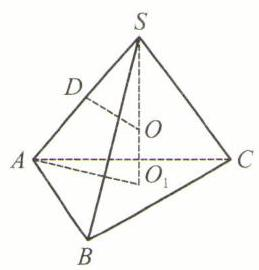
\includegraphics[width=0.2\textwidth]{bodyxb/src/bo_d20cdrf7aajc73bfmvhg_175_1166_326_259_270_0.jpg}
\end{center}


[第 231(1)题]

$\because {OA} = {OS} = r,\therefore {SD} = {AD} = \dfrac{1}{2}{SA} = \dfrac{1}{2}a$ ,

则 $\mathrm{{Rt}} \bigtriangleup  {SOD} \backsim  \mathrm{{Rt}} \bigtriangleup  {SAO}_{1},\therefore \dfrac{SO}{SA} = \dfrac{SD}{S{O}_{1}}$ ,即 $\dfrac{r}{a} = \dfrac{\dfrac{1}{2}a}{\dfrac{\sqrt{6}}{3}a}$ ,即 $a = \dfrac{2}{3}\sqrt{6}r$ , $\therefore \;{V}_{S - {ABC}} = \dfrac{1}{3}{S}_{\bigtriangleup {ABC}} \cdot  S{O}_{1} = \dfrac{8\sqrt{3}}{27}{r}^{3}$ .

(2)设内切球半径为 $r$ ,四个表面积分别为 ${S}_{1},{S}_{2},{S}_{3},{S}_{4}$ ,连接球心和 4 个顶点,原三棱锥被分为 4 个小的三棱锥,记体积分别为 ${V}_{1},{V}_{2},{V}_{3},{V}_{4}$ ,

$V = {V}_{1} + {V}_{2} + {V}_{3} + {V}_{4} = \dfrac{1}{3}{S}_{1}r + \dfrac{1}{3}{S}_{2}r + \dfrac{1}{3}{S}_{3}r + \dfrac{1}{3}{S}_{4}r = \dfrac{r}{3}\left( {{S}_{1} + {S}_{2} + {S}_{3} + {S}_{4}}\right)$

\begin{center}
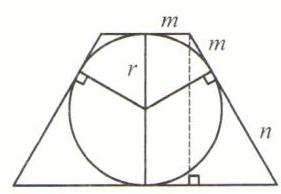
\includegraphics[width=0.2\textwidth]{bodyxb/src/bo_d20cdrf7aajc73bfmvhg_175_1141_874_281_194_0.jpg}
\end{center}


[第 232(1)题]

$= \dfrac{rS}{3}$ ,得 $r = \dfrac{3V}{S},\;\therefore \;{V}_{\text{ 球 }} = \dfrac{4}{3}\pi {r}^{3} = {36\pi } \cdot  \dfrac{{V}^{3}}{{S}^{3}}$ .

232. (1) 如图为过棱台上下底面一组平行的 4 条棱的中点的截面,不妨设上底边长 ${2m}$ ,下底边长 ${2n}$ ,内切球半径为 $r$ ,上底面面积为 ${S}_{1}$ ,下底面面积为 ${S}_{2}$ ,则 $h =$  $\sqrt{{\left( m + n\right) }^{2} - {\left( n - m\right) }^{2}} = \sqrt{4mn} = 2\sqrt{mn},r = \dfrac{h}{2} = \sqrt{mn}$ ,

$\therefore \dfrac{{V}_{\text{ 接台 }}}{{V}_{\text{ 球 }}} = \dfrac{\dfrac{1}{3} \cdot  h\left( {{S}_{1} + {S}_{2} + \sqrt{{S}_{1}{S}_{2}}}\right) }{\dfrac{4}{3}\pi {r}^{3}} = \dfrac{\dfrac{1}{3} \cdot  2\sqrt{mn} \cdot  \left( {4{m}^{2} + 4{n}^{2} + {4mn}}\right) }{\dfrac{4}{3}\pi  \cdot  \sqrt{mn} \cdot  {mn}} = \dfrac{2\left( {{m}^{2} + {n}^{2} + {mn}}\right) }{\pi mn}$ .

(2)如图为圆台的轴截面 ${ABCD}$ , $G$ 为等腰梯形 ${ABCD}$ 与其内切圆的一个切点,设球半径 $r$ ,圆台上、下底面圆的半径 ${r}_{1},{r}_{2}$ ,连接 ${OD},{OC},{OG}$ . 则 ${OD} \bot  {OC}$ .

\begin{center}
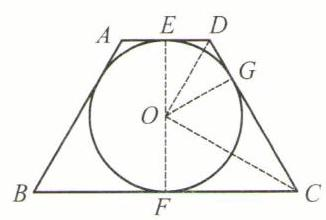
\includegraphics[width=0.2\textwidth]{bodyxb/src/bo_d20cdrf7aajc73bfmvhg_175_1097_1269_326_220_0.jpg}
\end{center}


[第 232(2)题]

$\therefore \;{r}^{2} = {DG} \cdot  {GC} = {DE} \cdot  {CF} = {r}_{1} \cdot  {r}_{2}.{S}_{\text{ 圆台侧 }} : {S}_{\text{ 球 }} = \left\lbrack  {\pi \left( {{r}_{1} + {r}_{2}}\right)  \cdot  {DC}}\right\rbrack   : {4\pi }{r}^{2} = 4 : 3$ .

又 $\because \;{DC} = {r}_{1} + {r}_{2},\;\therefore \;{\left( {r}_{1} + {r}_{2}\right) }^{2} : 4{r}^{2} = 4 : 3$ ,

$\therefore \;\left( {{r}_{1}^{2} + {r}_{2}^{2} + 2{r}_{1} \cdot  {r}_{2}}\right)  : 4{r}^{2} = 4 : 3.\;\therefore \;{r}_{1}^{2} + {r}_{2}^{2} = \dfrac{10}{3}{r}^{2},$

$\therefore \dfrac{{V}_{\text{ 圆台 }}}{{V}_{\text{ 球 }}} = \dfrac{\dfrac{1}{3}\left( {\pi {r}_{1}^{2} + \pi {r}_{1}{r}_{2} + \pi {r}_{2}^{2}}\right)  \cdot  {2r}}{\dfrac{4}{3}\pi {r}^{3}} = \dfrac{13}{6}$ .

233. (1) 设外接球半径为 $r$ ,则圆锥高为 ${rq},\;\therefore$ 底面半径 $R = \sqrt{{r}^{2} - {\left( rq - r\right) }^{2}} = r\sqrt{q\left( {2 - q}\right) },\dfrac{{S}_{\text{ 圆锥 }}}{{S}_{\text{ 球 }}} =$  $\dfrac{{\pi R}\left( {R + \sqrt{{r}^{2}{q}^{2} + {R}^{2}}}\right) }{{4\pi }{r}^{2}} = \dfrac{\left( {2 - q}\right) q + q\sqrt{2\left( {2 - q}\right) }}{4}.$

\begin{center}
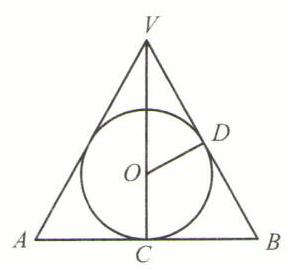
\includegraphics[width=0.2\textwidth]{bodyxb/src/bo_d20cdrf7aajc73bfmvhg_175_1138_1750_287_269_0.jpg}
\end{center}


[第 233(2)题]

(2)如图为圆锥的轴截面,设 ${AC} = R$ ,球半径 ${OD} = r$ ,圆锥高 ${VC} = h$ ,母线 ${VB} = l$ .

$\because \mathrm{{Rt}} \bigtriangleup  {VOD} \backsim  \mathrm{{Rt}} \bigtriangleup  {VBC},\;\therefore \;\dfrac{OD}{VO} = \dfrac{BC}{VB}$ ,即 $\dfrac{r}{h - r} = \dfrac{R}{l},\;\therefore \;\dfrac{r}{h} = \dfrac{R}{l + R}$ .

$\dfrac{{S}_{\text{ 球 }}}{{S}_{\text{ 锥 }}} = \dfrac{{4\pi }{r}^{2}}{{\pi R}\left( {R + l}\right) } = \dfrac{4{r}^{2}}{R\left( {R + l}\right) },\dfrac{{V}_{\text{ 球 }}}{{V}_{\text{ 锥 }}} = \dfrac{\dfrac{4}{3}\pi {r}^{3}}{\dfrac{1}{3}\pi {R}^{2}h} = \dfrac{4{r}^{2}}{R} \cdot  \dfrac{r}{Rh} = \dfrac{4{r}^{2}}{R\left( {R + l}\right) },\dfrac{{V}_{\text{ 球 }}}{{V}_{\text{ 锥 }}} = \dfrac{{S}_{\text{ 球 }}}{{S}_{\text{ 锥 }}}$ ,得证.

234. 设平面 ${PB}{D}_{1}$ 与棱 ${DC}$ 交点于点 $Q$ ,则截面 ${PBQ}{D}_{1}$ 是平行四边形, $\therefore$ 点 $P$ 到对角线 ${D}_{1}B$ 的距离最小时,截面面积最小. 当 $P$ 是 ${A}_{1}{B}_{1}$ 中点时, ${S}_{\text{ 截min }} = \dfrac{\sqrt{6}}{2}$ . 235. 作 ${AB} \bot$ 底面于点 $B$ ,则 ${AB}$ 为母线, $l$ 与底面交于点 $C$ ,连接 ${BC}$ . 则 $\angle {ACB} = \alpha$ ,而 ${CB}$ 为底面圆切线. $\therefore {OB} \bot  {BC}$ ,作 ${BD} \bot  {AC}$ 于点 $D$ ,连接 ${OD}$ , $\because {OB} \bot  {BC},{AB} \bot  {BC},\therefore {BC} \bot$ 平面 ${AOB},\therefore$ 平面 ${ACB} \bot$ 平面 ${AOB}$ . $\because {OB} \bot  {AC},{AC} \bot  {BD},\therefore {AC} \bot$ 平面 ${OBD},\therefore {OD} \bot  {AC}$ .

$\therefore {OD}$ 即为点 $O$ 到直线 $l$ 的距离, $\therefore {OD} = \sqrt{\left( {{a}^{2} - {b}^{2}}\right) {\cos }^{2}\alpha  + {b}^{2}}$ .

236. 把正四面体 ${ABCD}$ 的中心看成点 $O,4$ 条射线分别为 ${OA},{OB},{OC},{OD}$ .

设正四面体棱长为 1,则 ${OA} = {OB} = \dfrac{\sqrt{6}}{4}$ ,

$\cos \angle {AOB} = \dfrac{{\left( \dfrac{\sqrt{6}}{4}\right) }^{2} + {\left( \dfrac{\sqrt{6}}{4}\right) }^{2} - {\left( 1\right) }^{2}}{2 \cdot  \dfrac{\sqrt{6}}{4} \cdot  \dfrac{\sqrt{6}}{4}} =  - \dfrac{1}{3},\;\therefore \;$ 所求夹角的余弦值为 $- \dfrac{1}{3}$ .

237. 在平面 ${A}_{1}{B}_{1}{C}_{1}$ 内过点 $Q$ 作 ${QD} \bot  {A}_{1}{B}_{1}$ 于点 $D$ . 又 ${QD} \bot  {A}_{1}A,\therefore {QD} \bot$ 平面 $A{A}_{1}{B}_{1}B$ . 即 $\angle {QPD} = {30}^{ \circ  }$ .

作 ${PH} \bot$ 平面 ${BC}{C}_{1}{B}_{1}$ 于点 $H$ ,由题意可得 $\angle {PQH} = {30}^{ \circ  }$ ,且 ${PH}$ 的长等于底面三角形的高.

设 ${PH} = h$ ,则 ${PQ} = {2h}$ .

在 $\mathrm{{Rt}}\bigtriangleup {QDP}$ 中, ${PQ} = {2h},\angle {QPD} = {30}^{ \circ  },\therefore {DQ} = h$ ,即点 $Q$ 与点 ${C}_{1}$ 重合.

在 $\operatorname{Rt} \bigtriangleup  P{A}_{1}D$ 中, ${A}_{1}P = 2,{DP} = \sqrt{3}h,{A}_{1}D = \dfrac{\sqrt{3}h}{3}$ ,得 ${2}^{2} + {\left( \dfrac{\sqrt{3}}{3}h\right) }^{2} = {\left( \sqrt{3}h\right) }^{2}$ ,解得 $h = \dfrac{\sqrt{6}}{2}$ ,

$\therefore \;{A}_{1}{B}_{1} = \dfrac{\sqrt{6}}{2} \cdot  \dfrac{\sqrt{3}}{3} \cdot  2 = \sqrt{2}.\;\therefore \;V = \dfrac{\sqrt{3}}{4} \cdot  {\sqrt{2}}^{2} \cdot  3 = \dfrac{3\sqrt{3}}{2}$ .

238. 以四面体的各棱为侧面对角线,拼成一个长方体,设长方体长、宽、高为 $x,y,z$ . 则

(1) 由 $\left\{  {\begin{array}{l} {x}^{2} + {y}^{2} = {16}, \\  {y}^{2} + {z}^{2} = {25}, \\  {z}^{2} + {x}^{2} = {36}, \end{array}\text{ 得 }\left\{  \begin{array}{l} {x}^{2} = {13.5}, \\  {y}^{2} = {2.5},\text{ 则 }{x}^{2} \cdot  {y}^{2} \cdot  {z}^{2} = \dfrac{6075}{8}, \\  {z}^{2} = {22.5}, \end{array}\right. }\right.$ 所以 $x \cdot  y \cdot  z = \dfrac{45}{4}$ ,

即 $V = \dfrac{1}{3}{xyz} = \dfrac{{45}\sqrt{6}}{4} \cdot  \dfrac{1}{3} = \dfrac{15}{4}\sqrt{6}$ .

2) $\left\{  \begin{array}{l} {x}^{2} + {y}^{2} = {a}^{2}, \\  {y}^{2} + {z}^{2} = {b}^{2}, \\  {z}^{2} + {x}^{2} = {c}^{2}, \end{array}\right.$ 得 $\left\{  \begin{array}{l} {x}^{2} = \dfrac{{a}^{2} + {c}^{2} - {b}^{2}}{2}, \\  {y}^{2} = \dfrac{{a}^{2} + {b}^{2} - {c}^{2}}{2}, \\  {z}^{2} = \dfrac{{b}^{2} + {c}^{2} - {a}^{2}}{2}, \end{array}\right.$

得 ${xyz} = \sqrt{\dfrac{1}{8} \cdot  \left( {{a}^{2} + {c}^{2} - {b}^{2}}\right) \left( {{a}^{2} + {b}^{2} - {c}^{2}}\right) \left( {{b}^{2} + {c}^{2} - {a}^{2}}\right) }$ ,

即 $V = \dfrac{1}{3}{xyz} = \dfrac{1}{12} \cdot  \sqrt{2\left( {{a}^{2} + {b}^{2} - {c}^{2}}\right) \left( {{b}^{2} + {c}^{2} - {a}^{2}}\right) \left( {{c}^{2} + {a}^{2} - {b}^{2}}\right) }$ .

239. (1) $\because {S}_{\bigtriangleup {ABC}} = \dfrac{1}{2}\sqrt{{a}^{2}{b}^{2} + {b}^{2}{c}^{2} + {c}^{2}{a}^{2}},\therefore {V}_{P - {ABC}} = \dfrac{h}{6} \cdot  \sqrt{{a}^{2}{b}^{2} + {b}^{2}{c}^{2} + {c}^{2}{a}^{2}}$ .

${V}_{P - {ABC}} = {V}_{A - {PBC}} = \dfrac{1}{6}{abc},\;\therefore \;{abc} = h \cdot  \sqrt{{a}^{2}{b}^{2} + {b}^{2}{c}^{2} + {c}^{2}{a}^{2}}$ .

即 ${a}^{2}{b}^{2}{c}^{2} = {h}^{2}\left( {{a}^{2}{b}^{2} + {b}^{2}{c}^{2} + {c}^{2}{a}^{2}}\right) ,\;\therefore \;\dfrac{1}{{h}^{2}} = \dfrac{1}{{a}^{2}} + \dfrac{1}{{b}^{2}} + \dfrac{1}{{c}^{2}}$ .

(2) $\because V = {V}_{Q - {APB}} + {V}_{Q - {PBC}} + {V}_{Q - {PCA}} = \dfrac{1}{6}\left( {{abz} + {bcx} + {cay}}\right)  = \dfrac{1}{6}{abc},\;\therefore \;{abc} = {bcx} + {cay} + {abz}$ ,故 $\dfrac{x}{a} + \dfrac{y}{b} + \dfrac{z}{c} = 1$ .

240. $\because V = {V}_{A - {BCD}} = \dfrac{1}{3}{S}_{\bigtriangleup {BCD}} \cdot  a,{V}_{1} = {V}_{P - {BCD}} = \dfrac{1}{3} \cdot  {S}_{\bigtriangleup {BCD}} \cdot  {a}_{1},\therefore \dfrac{{a}_{1}}{a} = \dfrac{{V}_{1}}{V}$ ,

$\therefore \dfrac{{a}_{1}}{a} + \dfrac{{b}_{1}}{b} + \dfrac{{c}_{1}}{c} + \dfrac{{d}_{1}}{d} = \dfrac{{V}_{1} + {V}_{2} + {V}_{3} + {V}_{4}}{V} = \dfrac{V}{V} = 1$ .

241. 设点 $A\left( B\right) ,C\left( D\right)$ 到截面 ${EHFM}$ 的距离分别为 ${h}_{1},{h}_{2}$ .

$\because {V}_{B - {EFC}} = {V}_{B - {EHF}} + {V}_{C - {EHF}} = \dfrac{1}{3}{S}_{\bigtriangleup {EHF}} \cdot  \left( {{h}_{1} + {h}_{2}}\right) ,{V}_{A - {EFD}} = {V}_{A - {EMF}} + {V}_{D - {EMF}} = \dfrac{1}{3}{S}_{\bigtriangleup {EMF}} \cdot  \left( {{h}_{1} + {h}_{2}}\right)$ ,

又 ${V}_{B - {EFC}} = {V}_{A - {EFD}},\;\therefore \;{S}_{EHF} = {S}_{\bigtriangleup {EMF}}$ .

而 ${EF}$ 为 $\bigtriangleup {EHF}$ 与 $\bigtriangleup {EMF}$ 的公共边,

$\therefore$ 点 $H,M$ 到 ${EF}$ 距离相等,即 ${MH}$ 被 ${EF}$ 平分.

242. 由本书第 209 页例 8 的结论, ${V}_{\text{ 四面体 }{ABCD}} = \dfrac{1}{6}{a}^{2}h$ .

243. 在 $\alpha$ 内作平行四边形 ${AEFC}$ . 则 ${V}_{A - {BEF}} = {V}_{A - {BCE}} = {V}_{A - {BFC}} = \dfrac{a}{3}{S}_{\bigtriangleup {BFC}}$ .

记 $\angle {BCF} = \theta$ ,则 ${BC} = a,{CF} = {2a}\sin \left( {{150}^{ \circ  } - \theta }\right)$ ,

$\therefore {S}_{\bigtriangleup {BFC}} = \dfrac{1}{2}a\left\lbrack  {{2a}\sin \left( {{150}^{ \circ  } - \theta }\right) }\right\rbrack   \cdot  \sin \theta  = \dfrac{{a}^{2}}{2}\left\lbrack  {\cos \left( {{150}^{ \circ  } - {2\theta }}\right)  + \dfrac{\sqrt{3}}{2}}\right\rbrack   \leq  \dfrac{{a}^{2}}{2}\left( {1 + \dfrac{\sqrt{3}}{2}}\right)$ ,

$\therefore$ 当 $\angle {BCF} = {75}^{ \circ  },{AE} = {CF} = \dfrac{\sqrt{6} + \sqrt{2}}{2}a$ 时, ${V}_{\max } = \dfrac{2 + \sqrt{3}}{12}{a}^{3}$ .

244. 记边 ${BC},{CA},{AB}$ 上高分别为 ${h}_{a},{h}_{b},{h}_{c}$ ,则 ${V}_{1} : {V}_{2} : {V}_{3} = {h}_{a} : {h}_{b} : {h}_{c},\therefore {S}_{\bigtriangleup {PBC}} = {S}_{\bigtriangleup {PCA}} = {S}_{\bigtriangleup {PAB}}$ , $\therefore P$ 为 $\bigtriangleup {ABC}$ 的重心.

245. 如图, ${PC}$ 中点 $O$ 即外接球球心.

\begin{center}
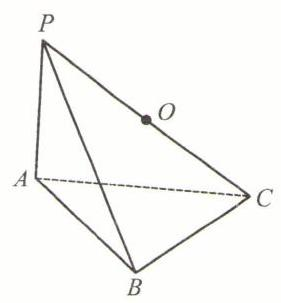
\includegraphics[width=0.2\textwidth]{bodyxb/src/bo_d20cdrf7aajc73bfmvhg_177_1130_607_281_303_0.jpg}
\end{center}


(第 245 题)

证明: $\because {PA} \bot$ 底面 ${ABC},\therefore {PA} \bot  {AC}$ ,

在 $\mathrm{{Rt}}\bigtriangleup {PAC}$ 中, $O$ 为斜边中点, $\therefore {PO} = {AO} = {CO}$ ,①

$\because {BC} \bot  {AB},{BC} \bot  {AP},\therefore {BC} \bot$ 平面 ${PAB},\therefore {BC} \bot  {PB}$ . 又 $O$ 为斜边 ${PC}$ 上中点, $\therefore {BO} = {PO} = {CO}$ ,

由①②得 ${AO} = {PO} = {CO} = {BO},\therefore O$ 为外接球球心. 得证.

246. 设内切球球心为 $O$ ,球半径为 $R.\because {V}_{P - {ABCD}} = {V}_{O - {ABCD}} + {V}_{O - {PAB}} + {V}_{O - {PBC}} + {V}_{O - {PCD}} + {V}_{O - {PAD}}$ , $\therefore R = 2$ .

247. 取 ${CD}$ 中点 $E.\;\because \;V = {V}_{C - {ABE}} + {V}_{D - {ABE}},V = {V}_{O - {ABC}} + {V}_{O - {BCD}} + {V}_{O - {ACD}} + {V}_{O - {ABD}}$ , $\therefore$ 内切球半径 $R = \dfrac{3\left( {\sqrt{13} - \sqrt{5}}\right) }{4},\therefore$ 点 $O$ 到 ${CD}$ 的距离为 $\dfrac{{39} - 3\sqrt{65}}{8}$ .

248. 如图,上下两层的球心组成一个正四面体,棱长为 ${2r}$ ,则 ${O}_{1}{O}_{2}$ 到 ${O}_{3}{O}_{4}$ 的距离 $h = \sqrt{{\left( \sqrt{3}r\right) }^{2} - {r}^{2}} = \sqrt{2}r$ .

\begin{center}
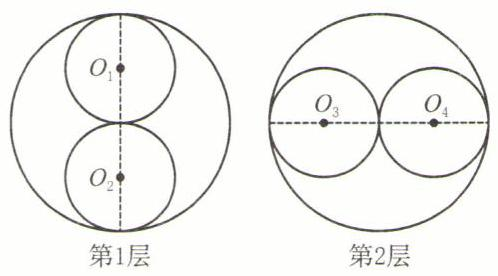
\includegraphics[width=0.4\textwidth]{bodyxb/src/bo_d20cdrf7aajc73bfmvhg_177_913_1042_498_276_0.jpg}
\end{center}


(第 248 题)

$\therefore$ 一共有 $\left\lbrack  \dfrac{{22r} - {2r}}{\sqrt{2}r}\right\rbrack   + 1 = {15}$ 层, $\therefore$ 最多 ${15} \times  2 = {30}$ (个)球.

249. 设两正方体棱长分别为 $x\mathrm{\;{cm}},y\mathrm{\;{cm}}$ ,则 $x + y = {10}$ .

$V = {x}^{3} + {y}^{3} = \left( {x + y}\right) \left( {{x}^{2} - {xy} + {y}^{2}}\right)  = \left( {x + y}\right) \left\lbrack  {{\left( x + y\right) }^{2} - {3xy}}\right\rbrack  ,$  $\therefore {xy} = \dfrac{{1000} - V}{30}$ ,则 $x,y$ 是关于 $t$ 的一元二次方程 ${t}^{2} - {10t} +$  $\dfrac{{1000} - V}{30} = 0$ 的两个实根.

$\Delta  = {100} - \dfrac{4\left( {{1000} - V}\right) }{30} \geq  0$ ,得 $V \geq  {250},\;\therefore \;$ 当 $x = y = 5\mathrm{\;{cm}}$ 时, ${V}_{\min } = {250}{\mathrm{\;{cm}}}^{3}$ .

250. 设外接球球心为 $O,{MN} = d,{PQ} = l,a,b$ 所成角为 $\theta$ . 过平面直线 $a,b$ 作两平行平面 ${\alpha }_{1},{\alpha }_{2}$ .

\begin{center}
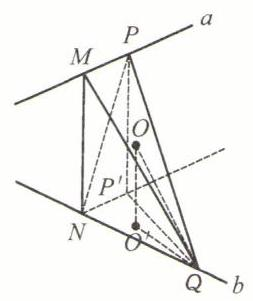
\includegraphics[width=0.2\textwidth]{bodyxb/src/bo_d20cdrf7aajc73bfmvhg_177_1158_1501_253_301_0.jpg}
\end{center}


(第 250 )题

作 $P{P}^{\prime } \bot  {\alpha }_{2}$ 于点 ${P}^{\prime }$ ,则 $P{P}^{\prime } = {MN} = d$ ,则 ${P}^{\prime }Q = \sqrt{{l}^{2} - {d}^{2}},\angle {P}^{\prime }{NQ} = \theta$ 或 $\pi  - \theta$ ,

设 $\bigtriangleup N{P}^{\prime }Q$ 外接圆圆心为 ${O}^{\prime }$ ,由正弦定理得 ${O}^{\prime }Q = \dfrac{\sqrt{{l}^{2} - {d}^{2}}}{2\sin \theta }$ .

在 $\mathrm{{Rt}} \bigtriangleup  {OO}^{\prime }Q$ 中, ${OQ} = \sqrt{O{O}^{\prime 2} + {O}^{\prime }{Q}^{2}} = \sqrt{\dfrac{{l}^{2} - {d}^{2}}{4{\sin }^{2}\theta } + \dfrac{{d}^{2}}{4}} = \dfrac{\sqrt{{l}^{2} - {d}^{2}{\cos }^{2}\theta }}{2\sin \theta }$ .

251. (1) 取 ${BC}$ 中点 ${O}_{1}$ ,连接 $O{O}_{1}.\because {O}_{1}$ 是以 ${BC}$ 为直径的圆的圆心,

$\therefore O{O}_{1} \bot   \odot  {O}_{1}$ ,即 $O{O}_{1} \bot$ 底面 ${BCD}$ . 又 $\because O{O}_{1} \subset$ 平面 ${ABC}$ ,

$\therefore$ 平面 ${ABC} \bot$ 平面 ${BCD}$ ,即平面 ${ACB} \bot  \alpha$ .

(2) $\because$ 平面 ${OED} \bot  \alpha$ ,平面 ${ACB} \bot  \alpha$ ,平面 ${OED} \cap$ 平面 ${ACB} = {OE}$ , $\therefore {OE} \bot  \alpha$ ,

$\therefore E$ 与 ${O}_{1}$ 重合, $\therefore \bigtriangleup {OED} \cong  \bigtriangleup {OEB}$ .

则 $\angle {ODE} = \angle {ABE} = \theta$ . 设球的半径为 $R$ ,则在 $\mathrm{{Rt}} \bigtriangleup  {OED}$ 中, ${OE} = R\sin \theta ,{ED} = R\cos \theta ,{S}_{\bigtriangleup {OED}} = \dfrac{1}{4}{R}^{2}\sin {2\theta },\dfrac{{S}_{\bigtriangleup {OED}}}{{S}_{\text{ 侧 }}}$

$= \dfrac{\dfrac{1}{4}{R}^{2}\sin {2\theta }}{\pi {R}^{2}} = \dfrac{\sin {2\theta }}{4\pi }.\;\therefore \;\theta  = \dfrac{\pi }{4}$ 时,面积之比最大.

